\subsection{Monte Carlo Statistical Uncertainties}
\label{sec:gbb-systs:MCstat}

The MC stats uncertainties are evaluated by re-sampling the response matrices from the nominal response matrix with associated MC stats uncertainty. In order to properly include correlations, the fake and inefficiency factors are set to unity (i.e. only events which pass both the detector-level and particle-level event selections are considered).

\subsection{Experimental Systematic Uncertainties}
\label{sec:gbb-systs:exp}

\begin{enumerate}
\item \textbf{R=1.0 jet JES and JER:} JES and JER uncertainty definitions can be found in Sec.\ref{sec:vbf-uncertainties}
    
%The uncertainty breakdown is shown in Fig.~\ref{fig:syst_overview_deltaR3}.
%\begin{figure}[htpb!]
%\begin{center}
%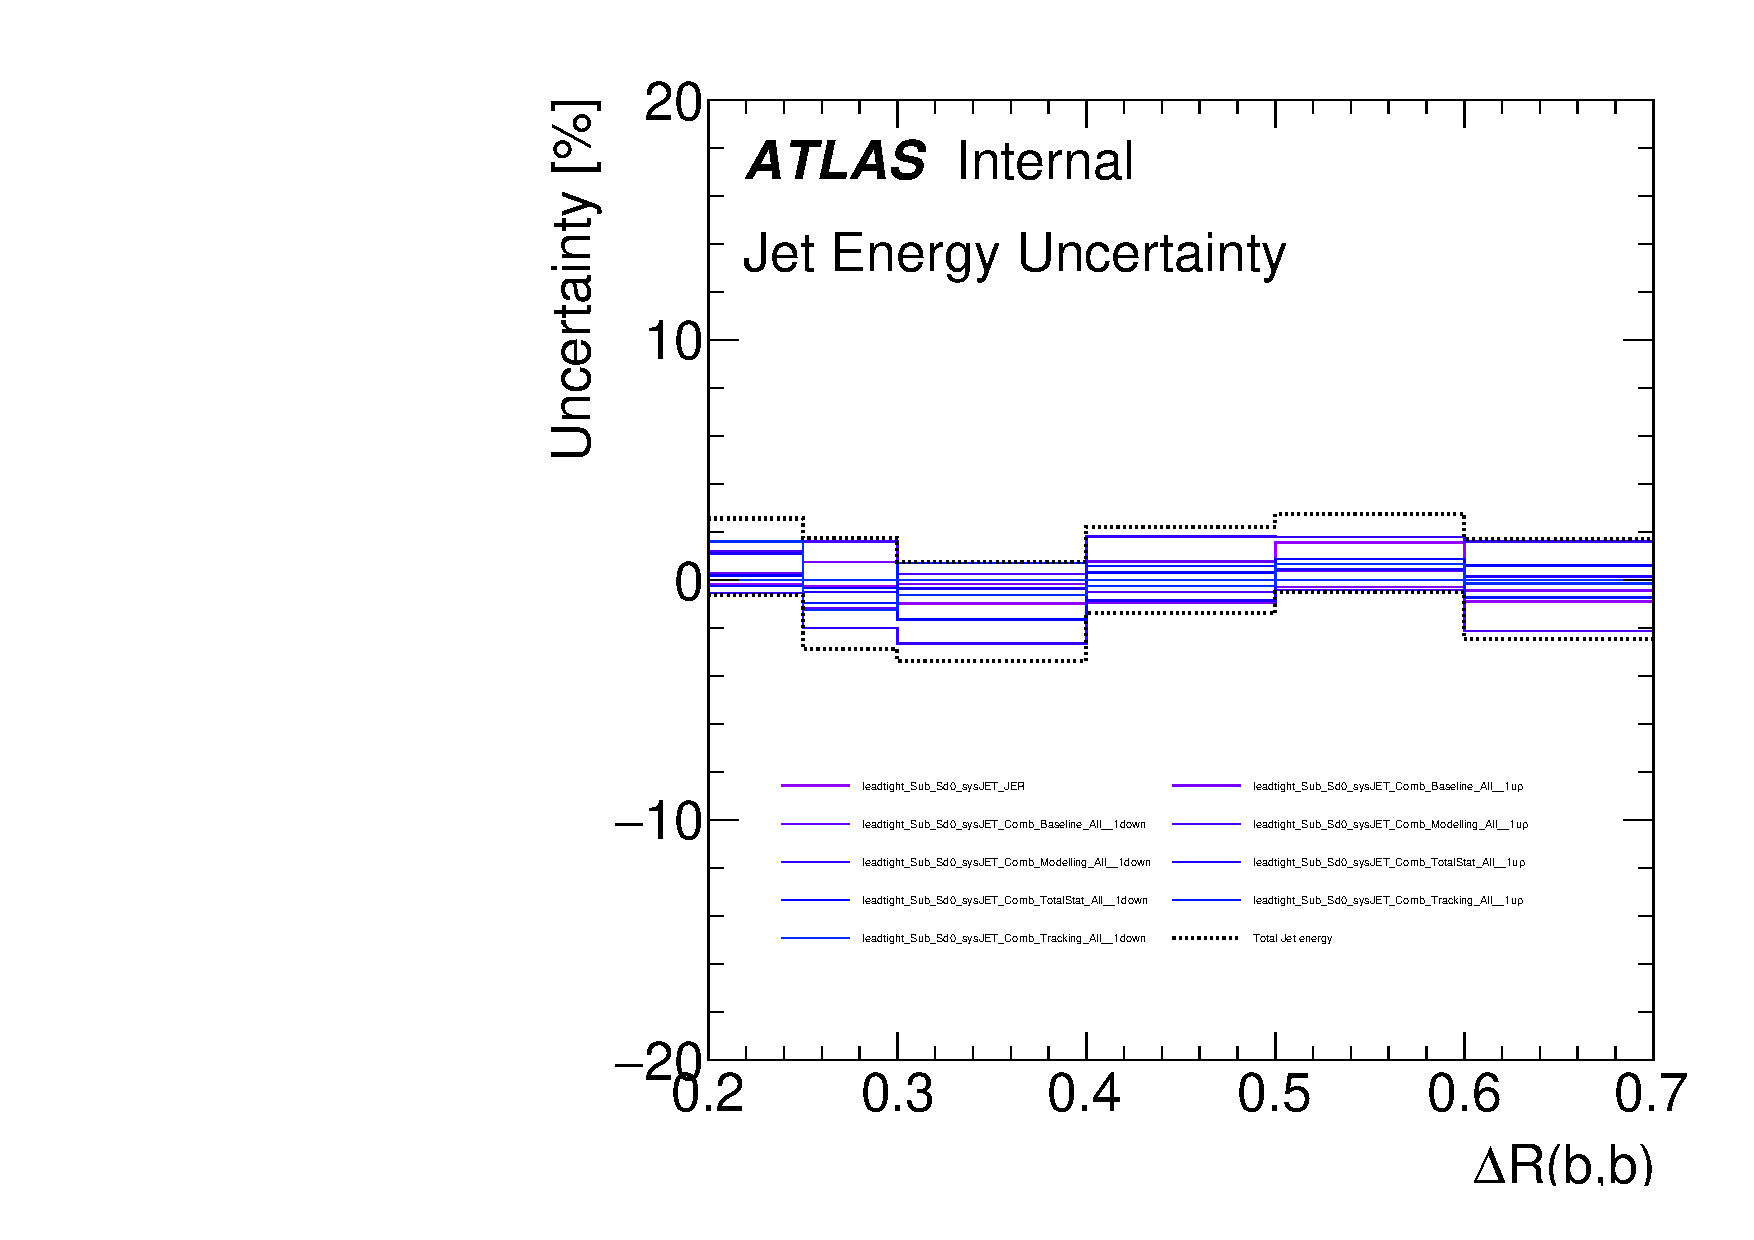
\includegraphics[width=0.45\linewidth]{figures/gbb/Unfolding/dR4_uncert_summary.pdf}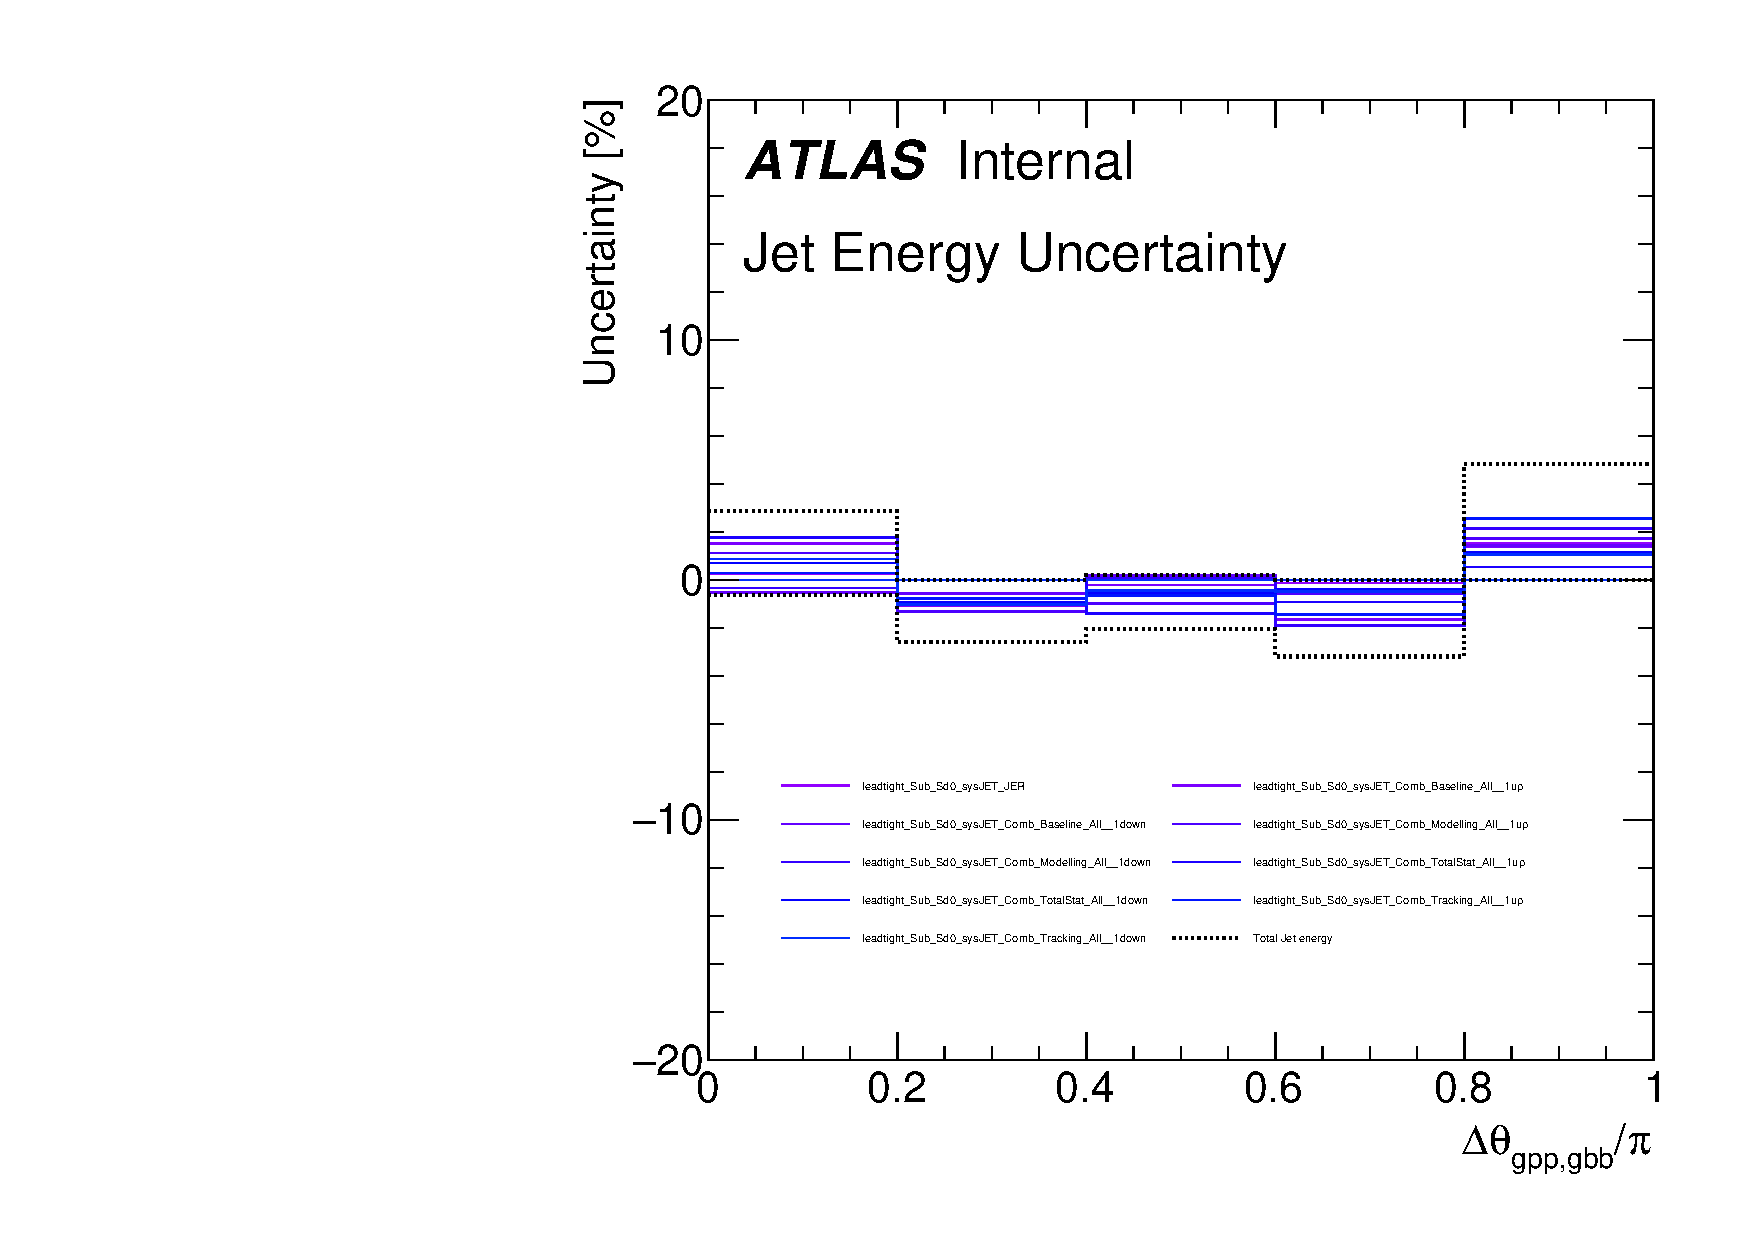
\includegraphics[width=0.45\linewidth]{figures/gbb/Unfolding/dphi4_uncert_summary.pdf}\\
%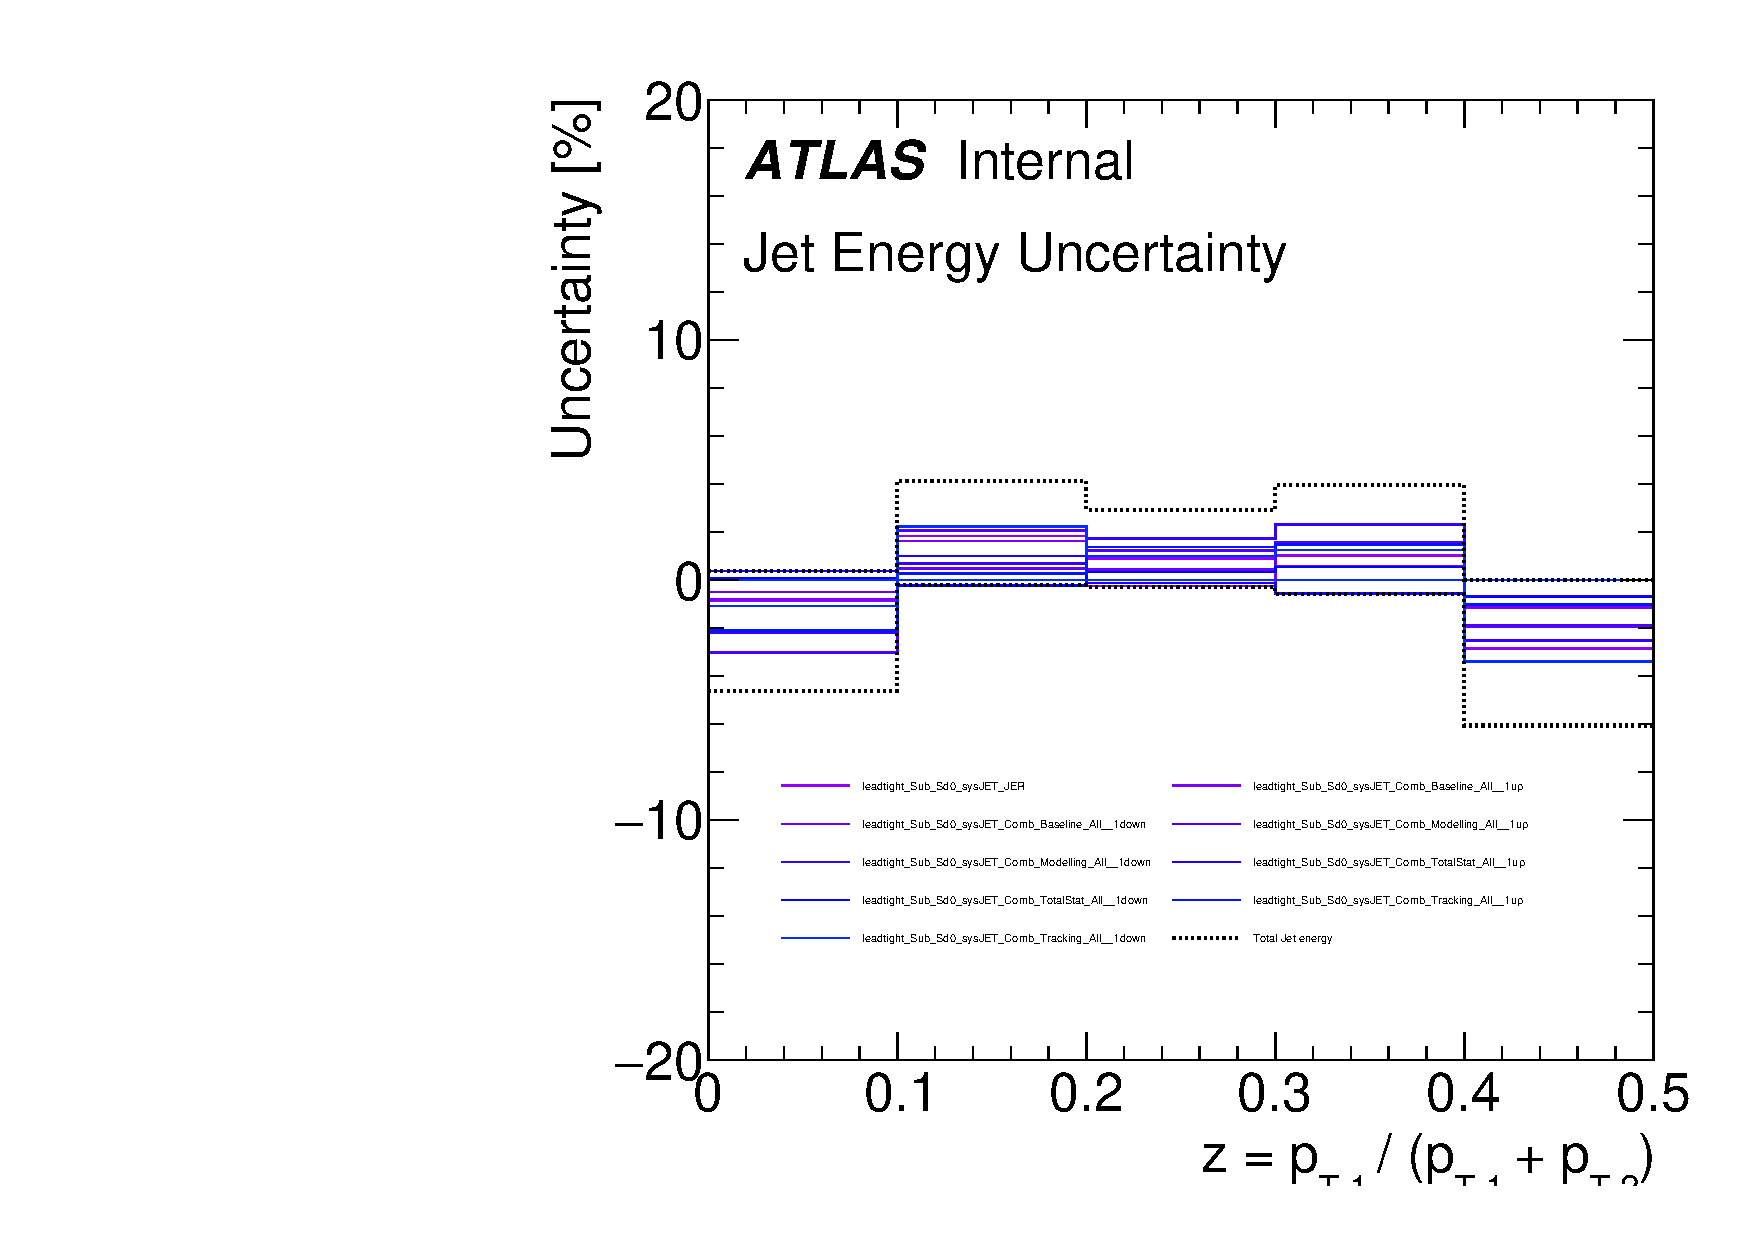
\includegraphics[width=0.45\linewidth]{figures/gbb/Unfolding/ZpT4_uncert_summary.pdf}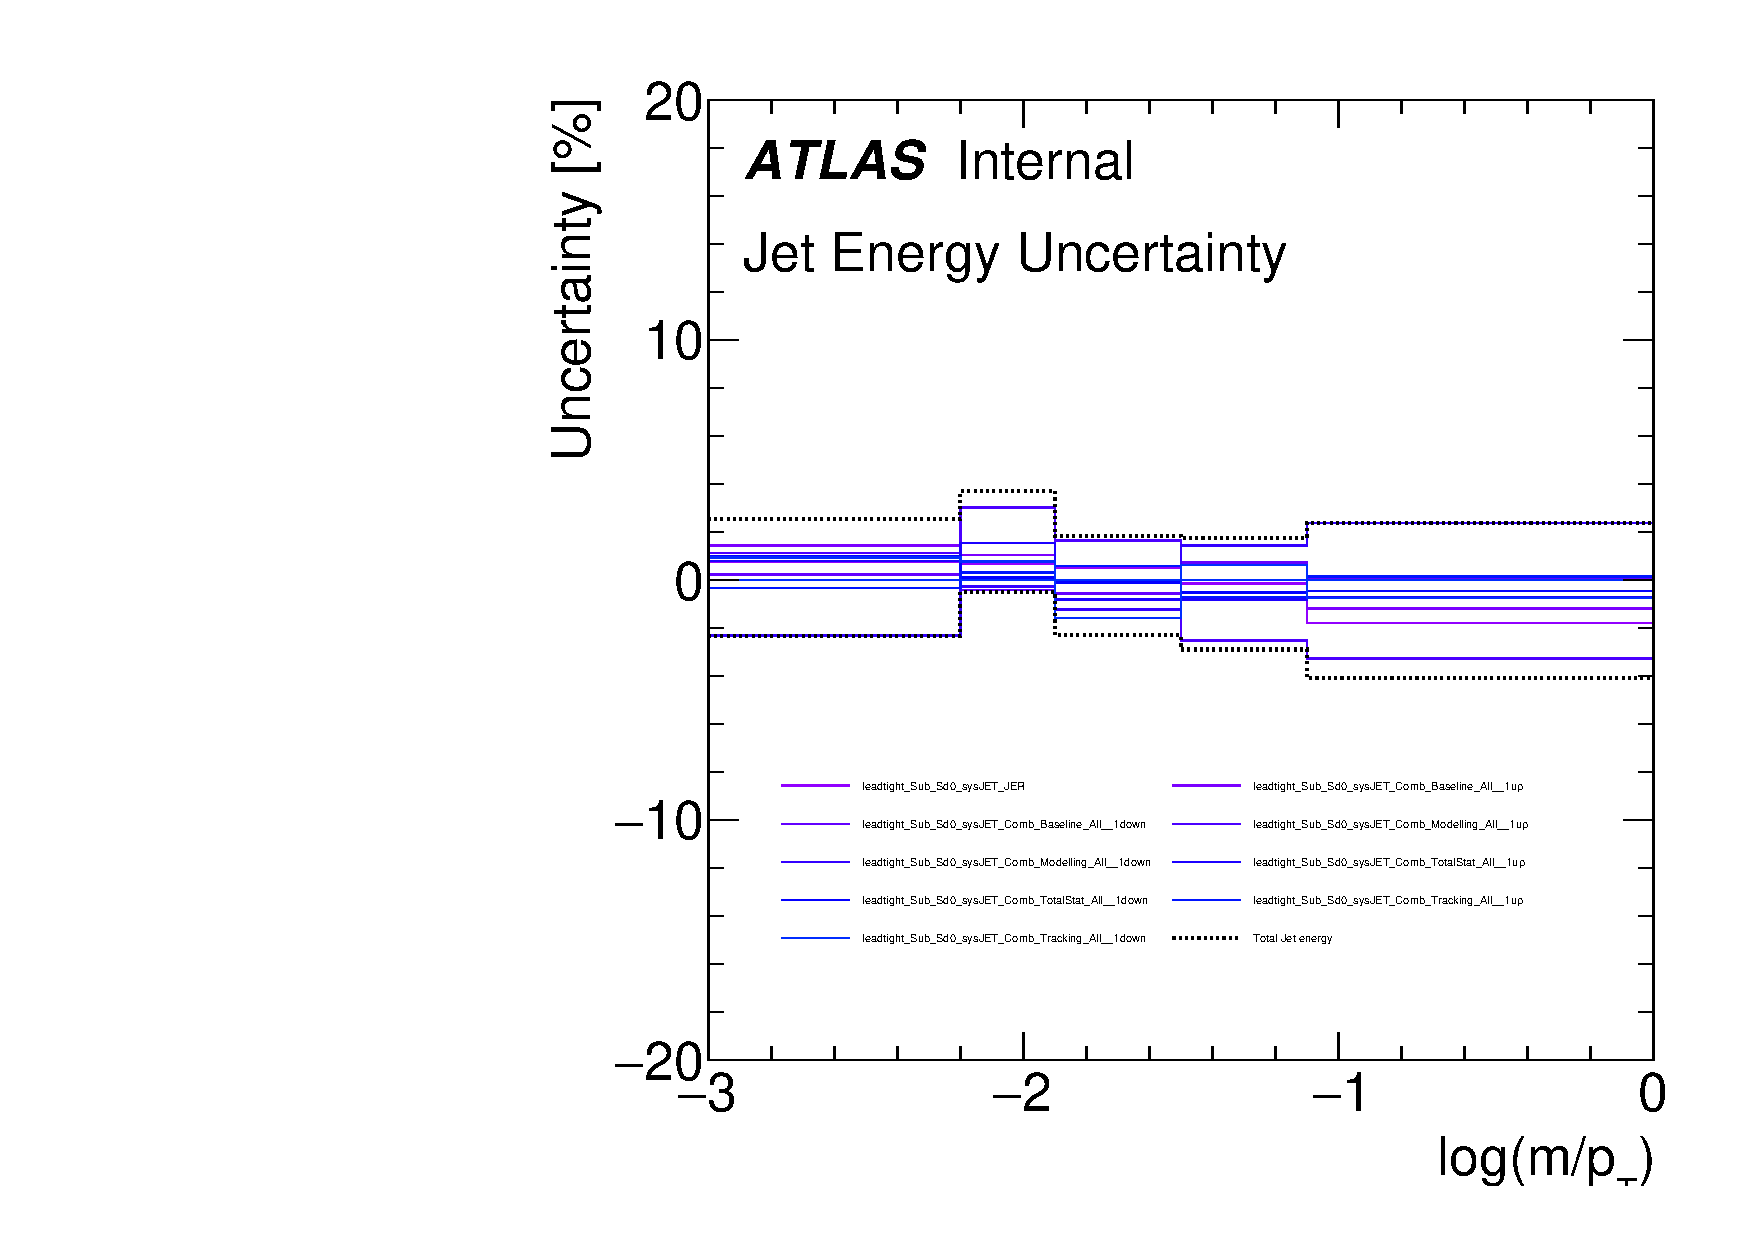
\includegraphics[width=0.45\linewidth]{figures/gbb/Unfolding/fracmasspt4_uncert_summary.pdf}
%\caption[]{A summary of the jet energy systematic uncertainties for all four observables. } 
%\label{fig:syst_overview_deltaR3}
%\end{center}
%\end{figure}

  \item \textbf{$b$-tagging scale factors:} \btagging uncertainty definitions can be found in Sec.\ref{sec:vbf-uncertainties}
  
%\begin{figure}[htpb!]
%\begin{center}
%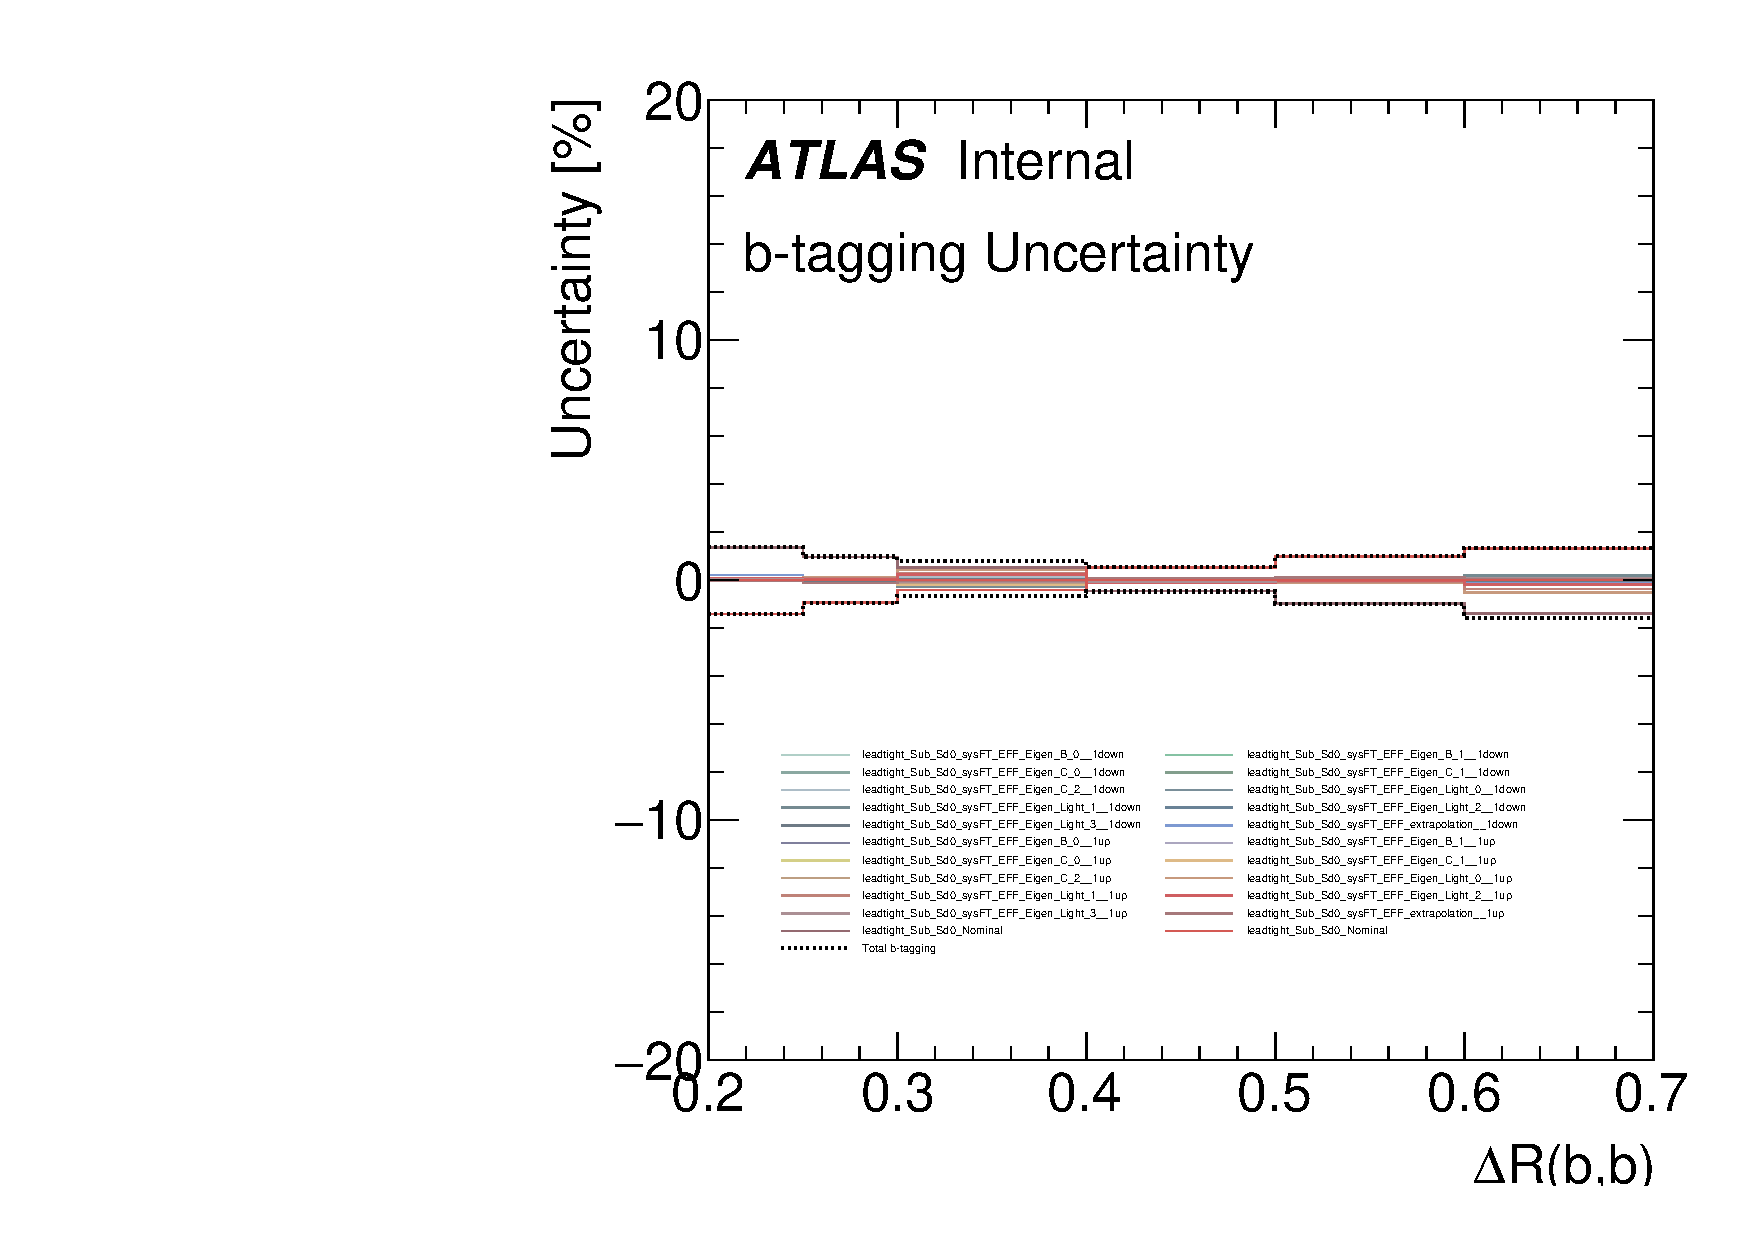
\includegraphics[width=0.45\linewidth]{figures/gbb/Unfolding/dR3_uncert_summary.pdf}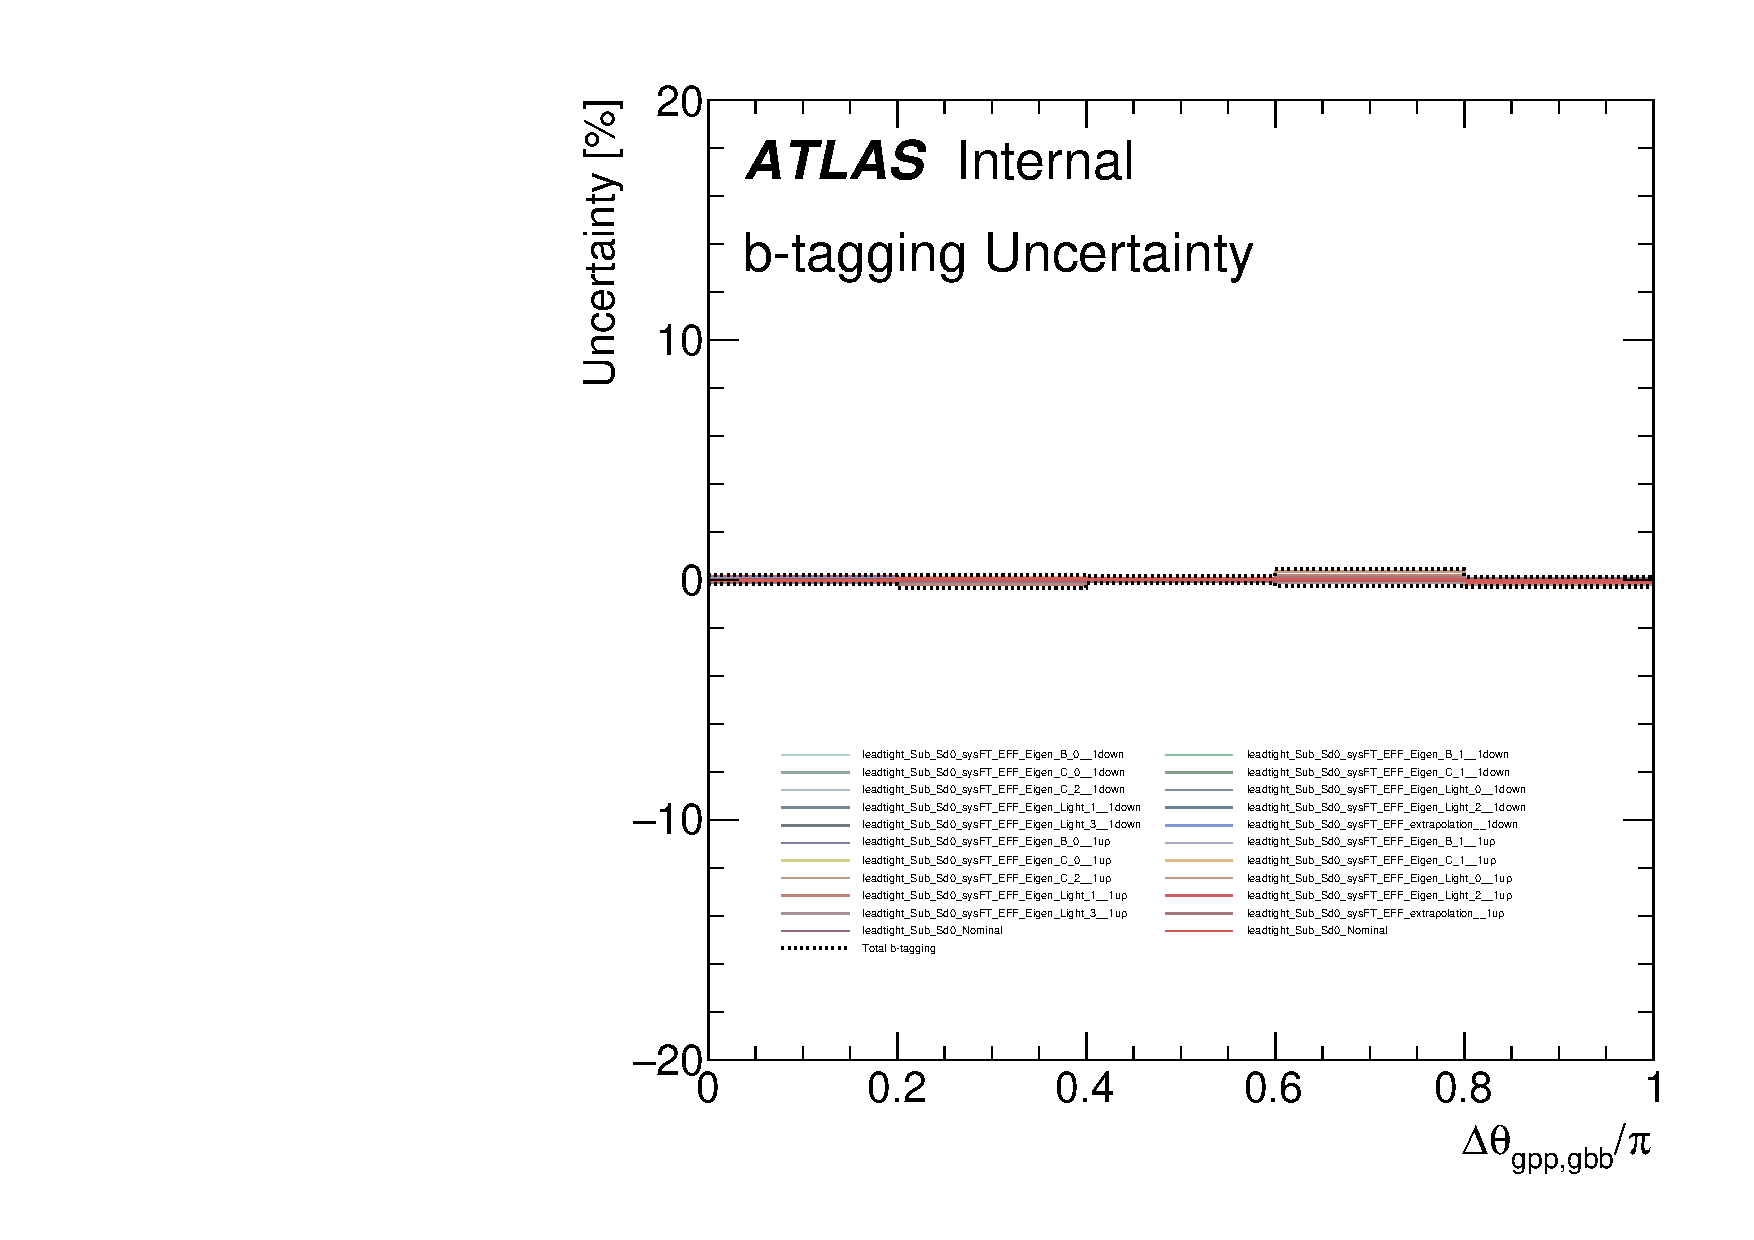
\includegraphics[width=0.45\linewidth]{figures/gbb/Unfolding/dphi3_uncert_summary.pdf}\\
%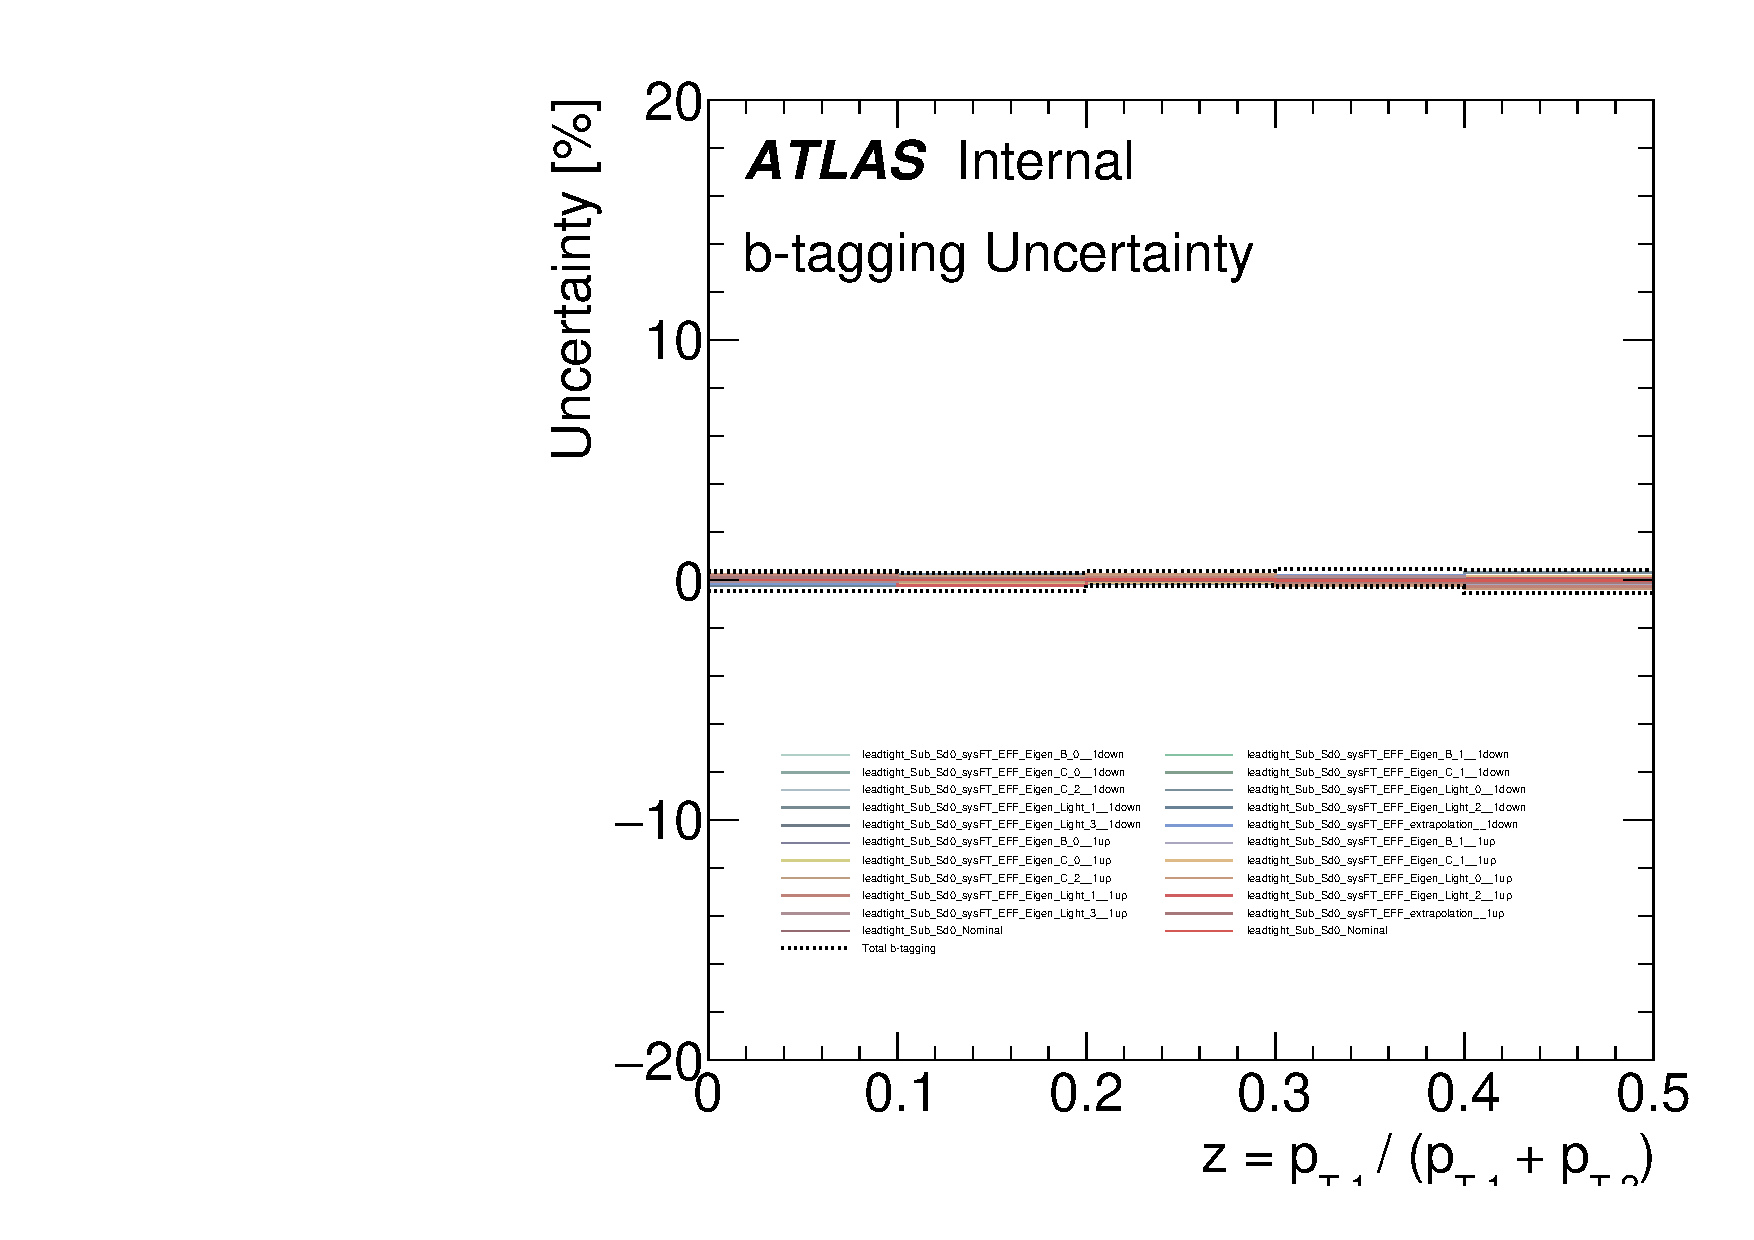
\includegraphics[width=0.45\linewidth]{figures/gbb/Unfolding/ZpT3_uncert_summary.pdf}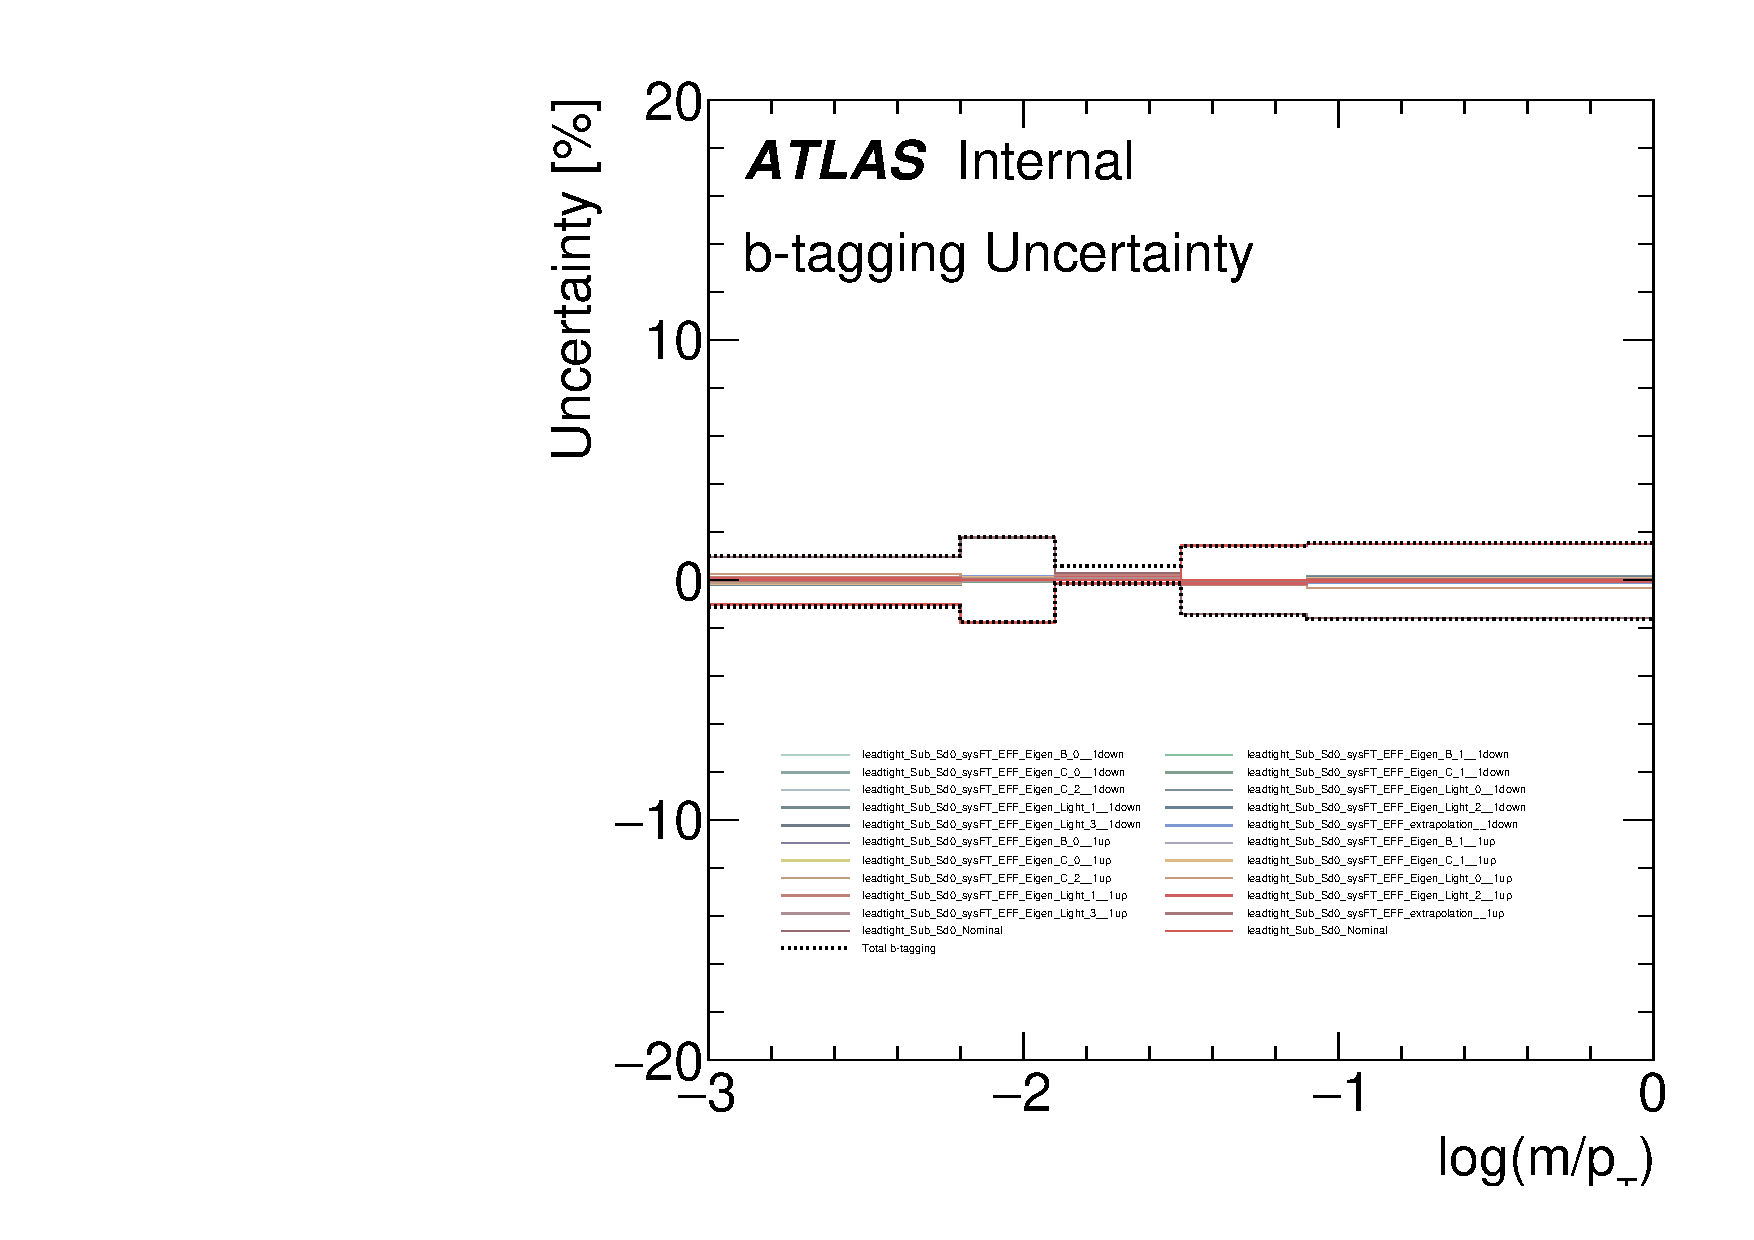
\includegraphics[width=0.45\linewidth]{figures/gbb/Unfolding/fracmasspt3_uncert_summary.pdf}
%\caption[]{A summary of the $b$-tagging systematic uncertainties for all four observables. } 
%\label{fig:syst_overview_deltaR3b}
%\end{center}
%\end{figure}
  
  \item \textbf{Tracking:} There are five sources : inclusive efficiency, tracking in dense environment modeling uncertainties, fake rate, sagitta bias, and $d_0$ bias/resolution. The inclusive efficiency uncertainty is due to the material uncertainty.  The total uncertainty is 0.5\% for $|\eta| < 0.1$ and grows to 2.7\% by $2.3 < |\eta| < 2.5$.  The uncertainty on the tracking efficiency inside dense environments is due to the modeling of pixel cluster merging applied to tracks with $\Delta R < 0.1$~\cite{Aaboud:2017all,ATL-PHYS-PUB-2016-007,ATL-PHYS-PUB-2017-016}. Fake tracks arise from random combinatorics of hits. A 27\% uncertainty is applied to the fake rate. The sagitta bias stem from weak modes and can bias the track \pt. %The uncertainty breakdown is shown in Fig.~\ref{fig:syst_overview_deltaR1}.  
  
%    \begin{figure}[htpb!]
%\begin{center}
%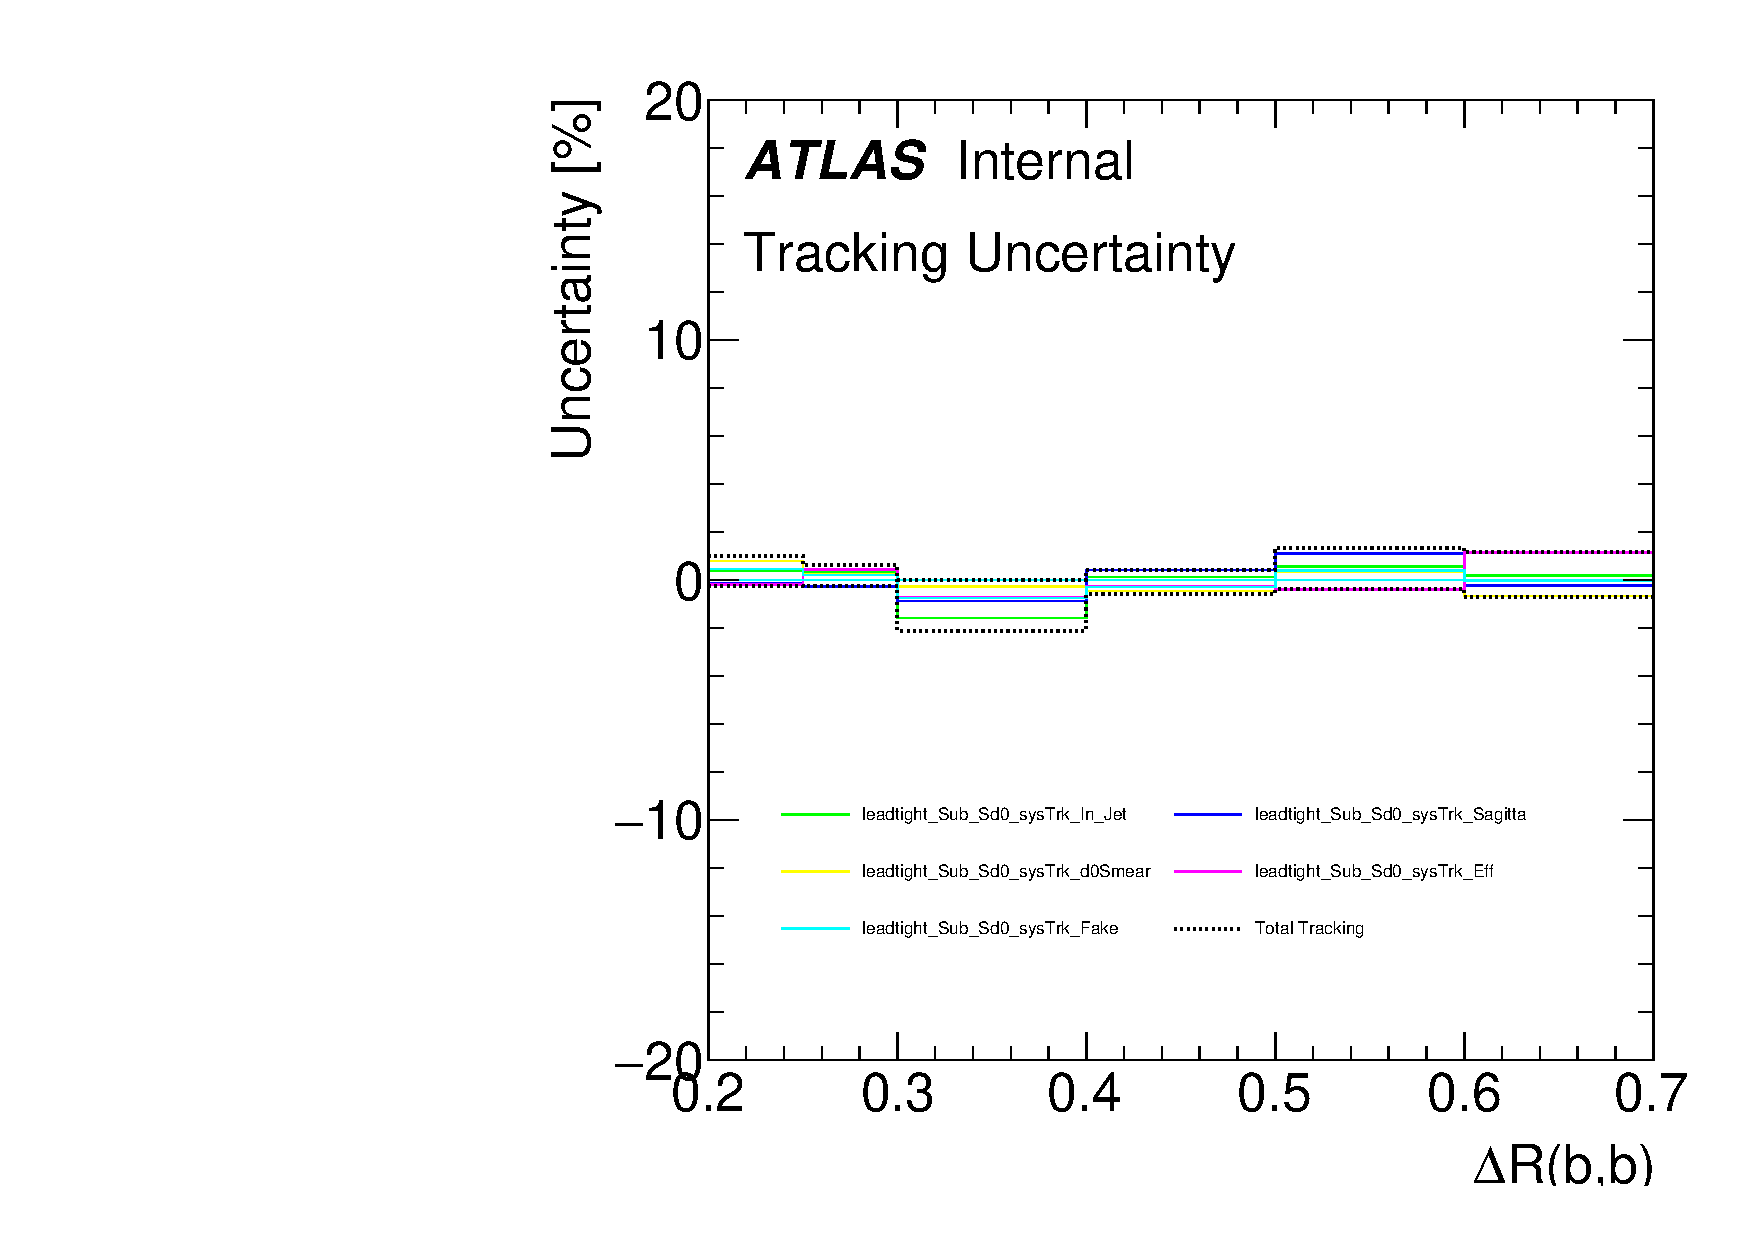
\includegraphics[width=0.45\linewidth]{figures/gbb/Unfolding/dR1_uncert_summary.pdf}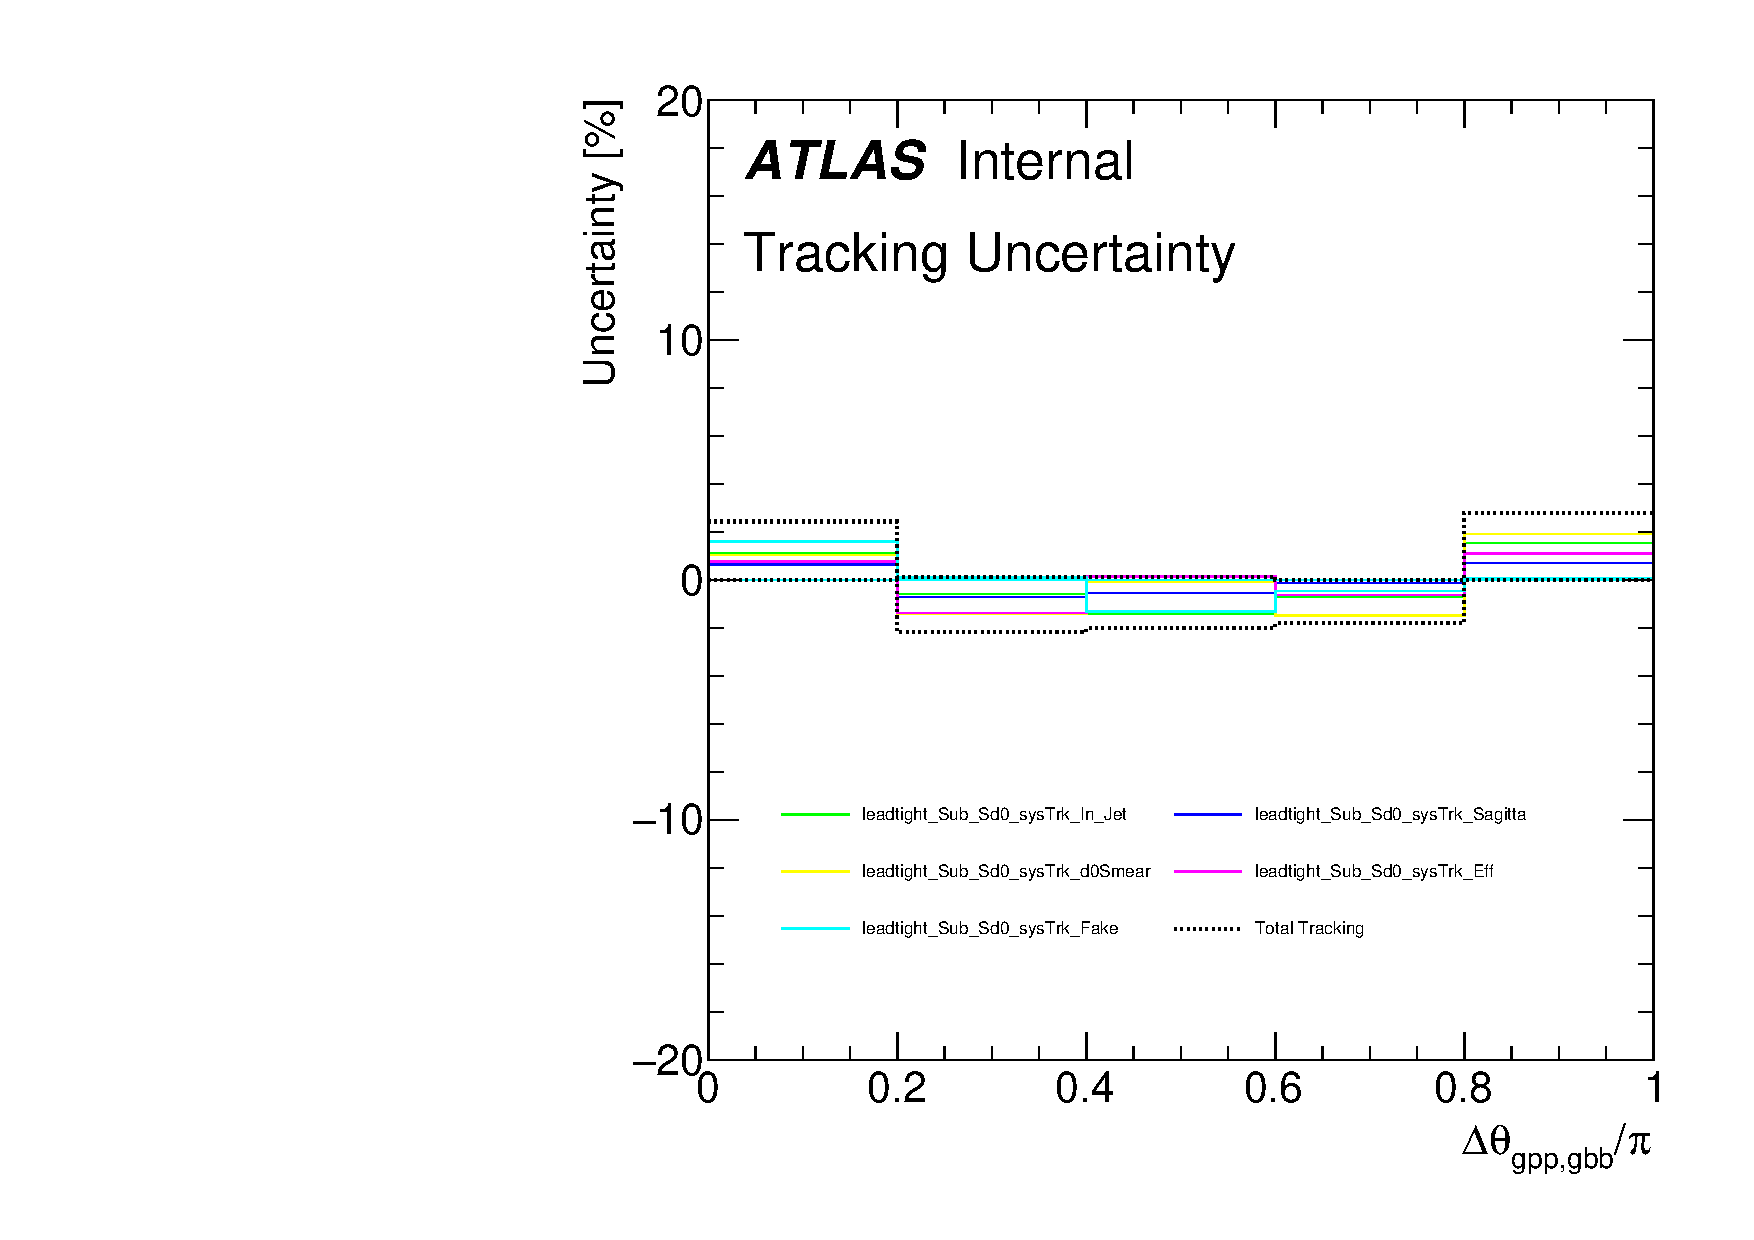
\includegraphics[width=0.45\linewidth]{figures/gbb/Unfolding/dphi1_uncert_summary.pdf}\\
%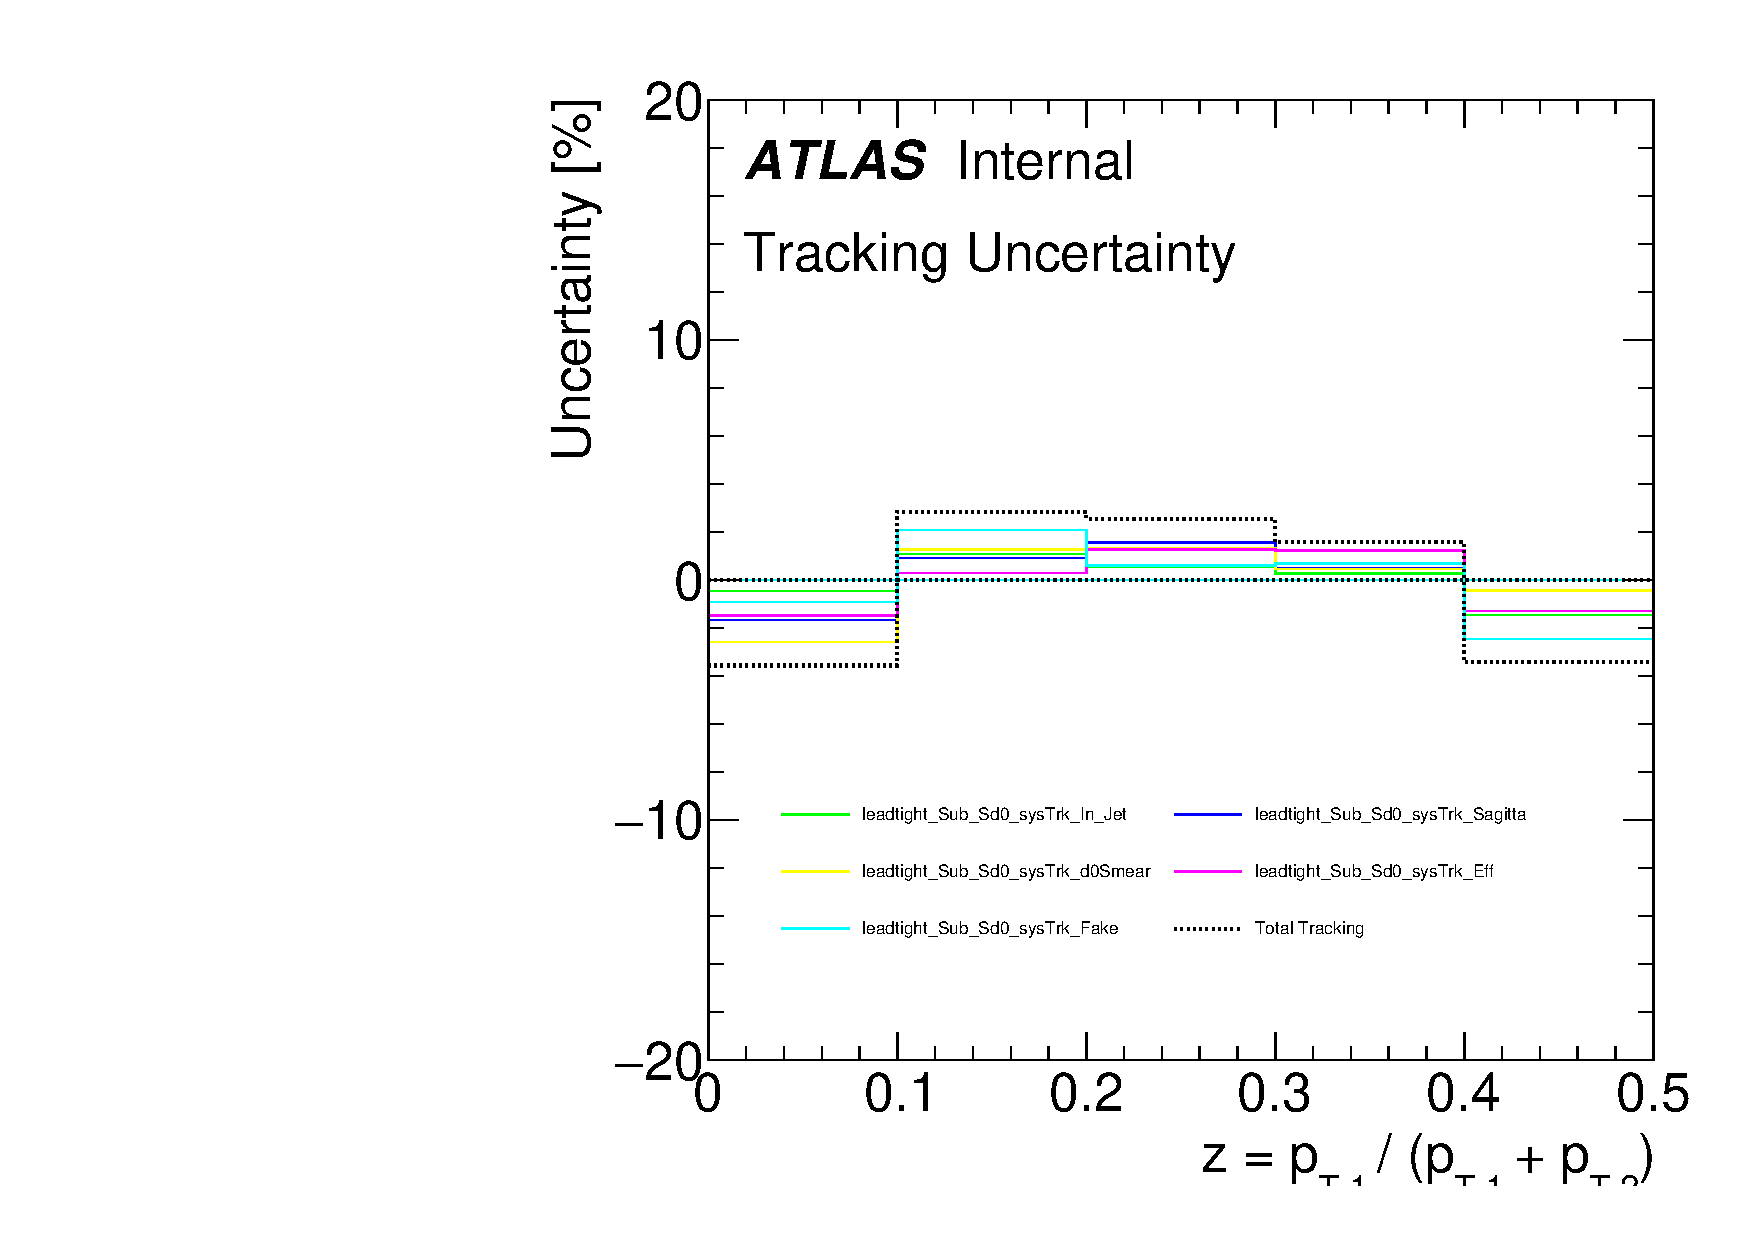
\includegraphics[width=0.45\linewidth]{figures/gbb/Unfolding/ZpT1_uncert_summary.pdf}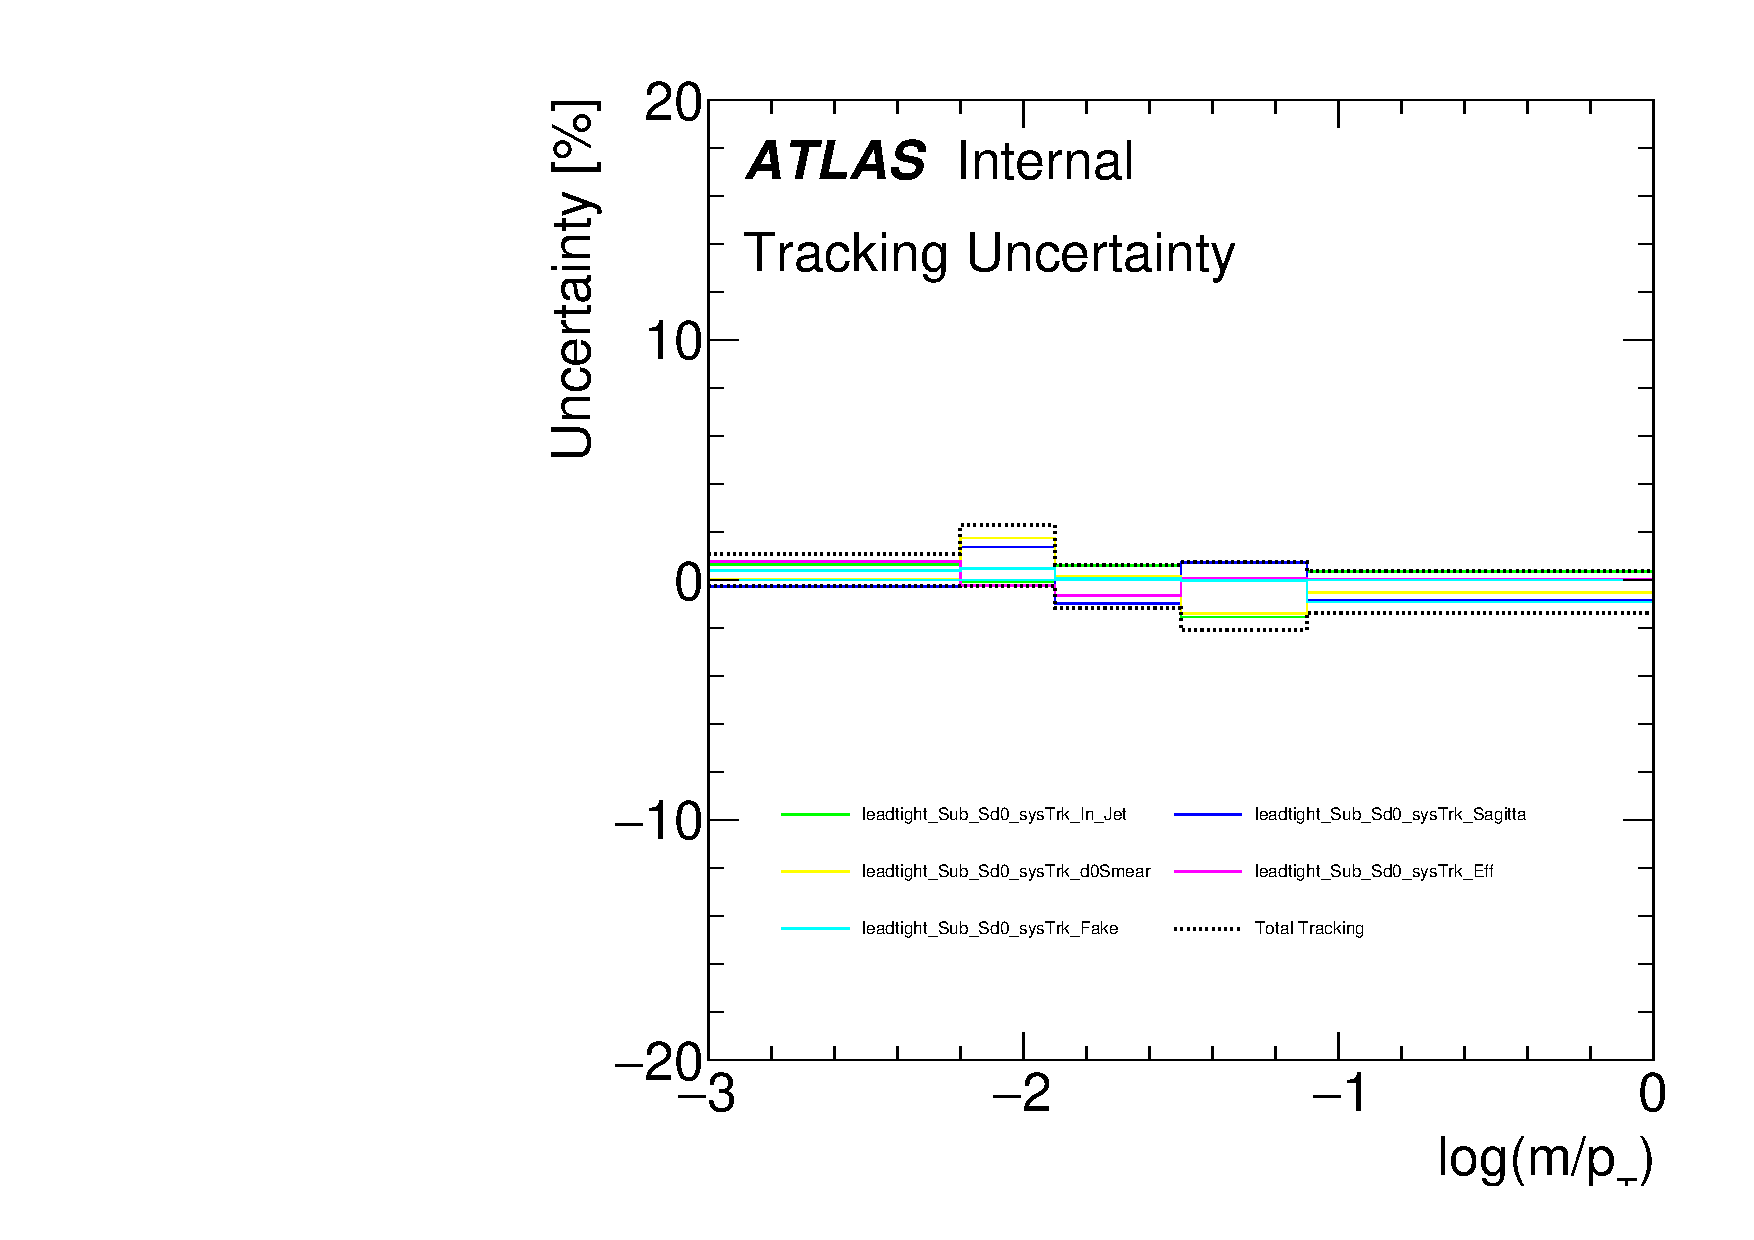
\includegraphics[width=0.45\linewidth]{figures/gbb/Unfolding/fracmasspt1_uncert_summary.pdf}
%\caption[]{A summary of the tracking systematic uncertainties for all four observables. } 
%\label{fig:syst_overview_deltaR1}
%\end{center}
%\end{figure}
  
\end{enumerate}

\subsection{Background Subtraction Uncertainty}
\label{sec:gbb-systs:background}

See Sec.~\ref{sec:gbb-sub_systematics} for definitions. These are treated as fully correlated with the corresponding sources described elsewhere in this section.%The uncertainty breakdown is shown in Fig.~\ref{fig:syst_overview_deltaR2}.
  
%  \begin{figure}[htpb!]
%\begin{center}
%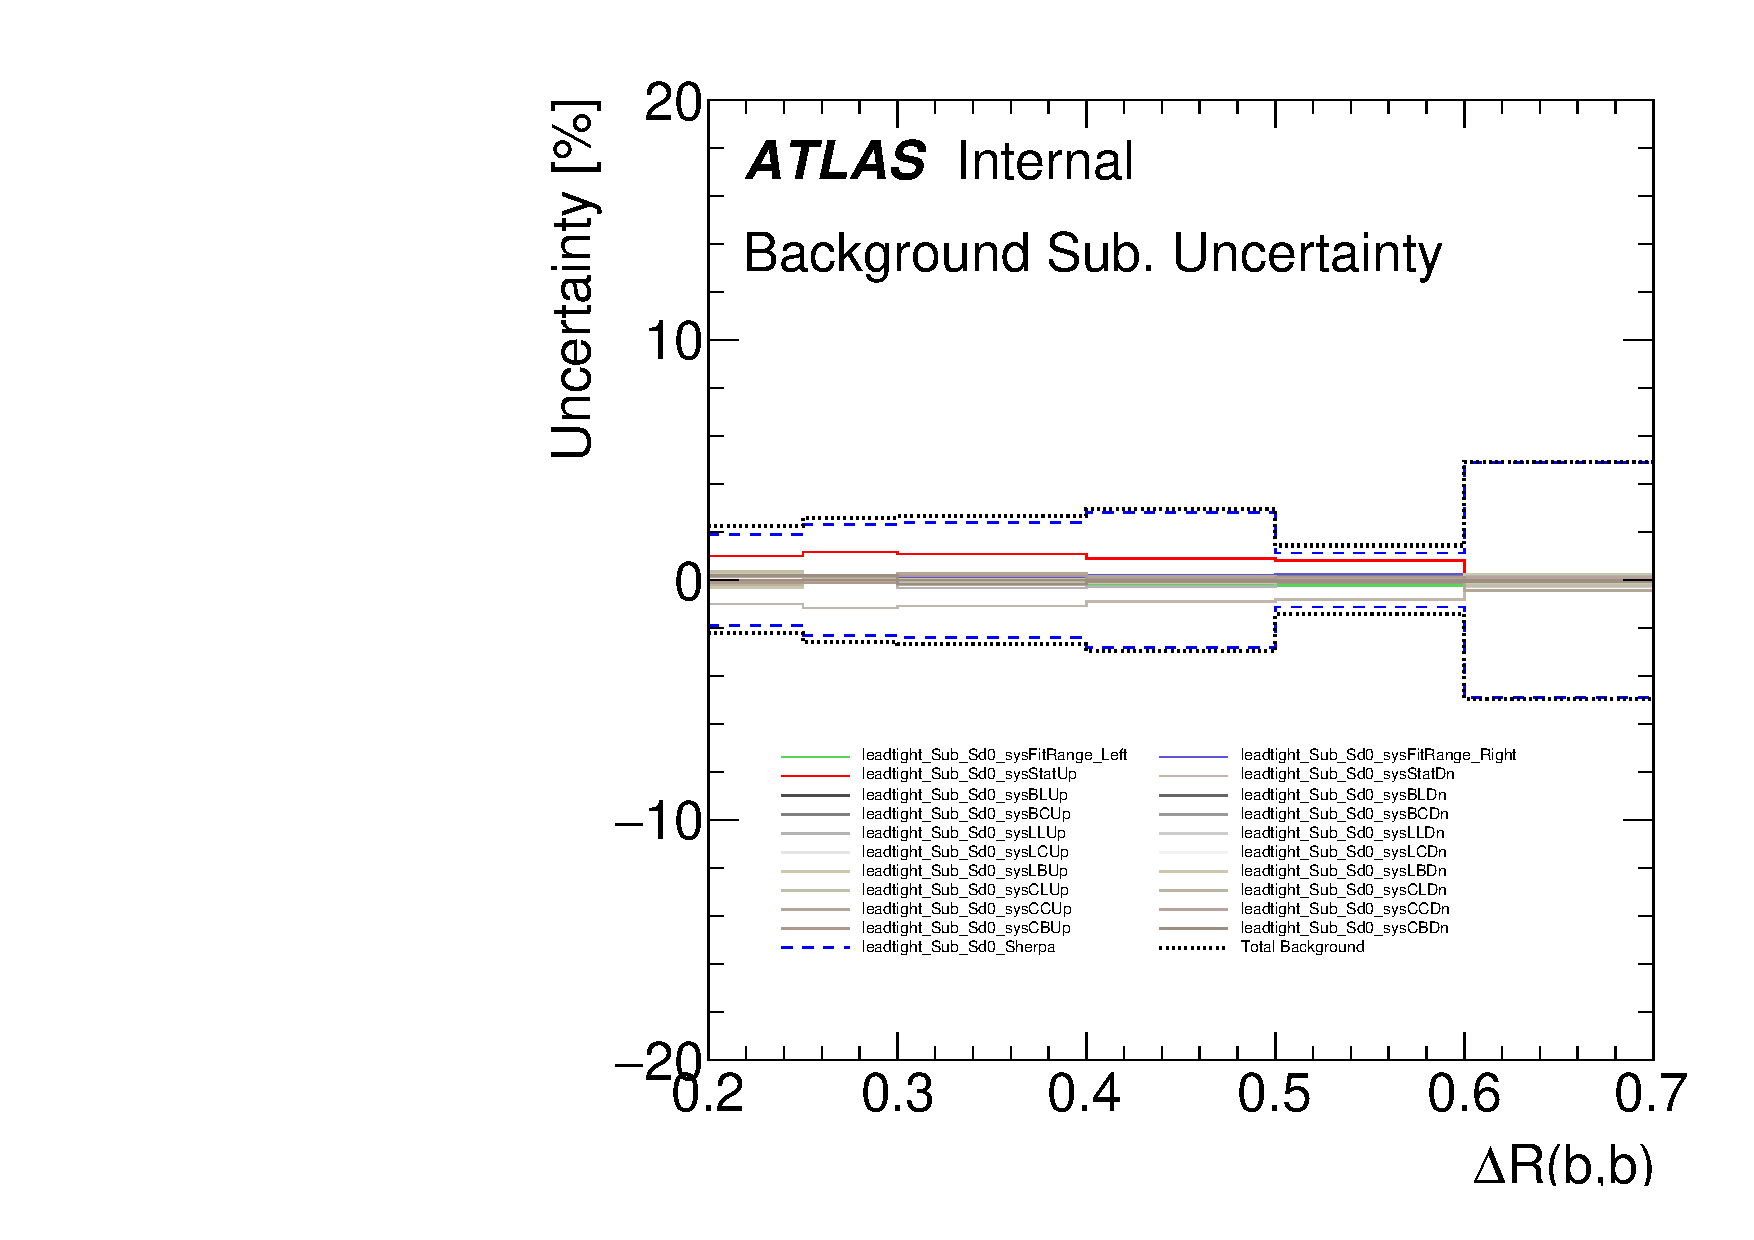
\includegraphics[width=0.45\linewidth]{figures/gbb/Unfolding/dR2_uncert_summary.pdf}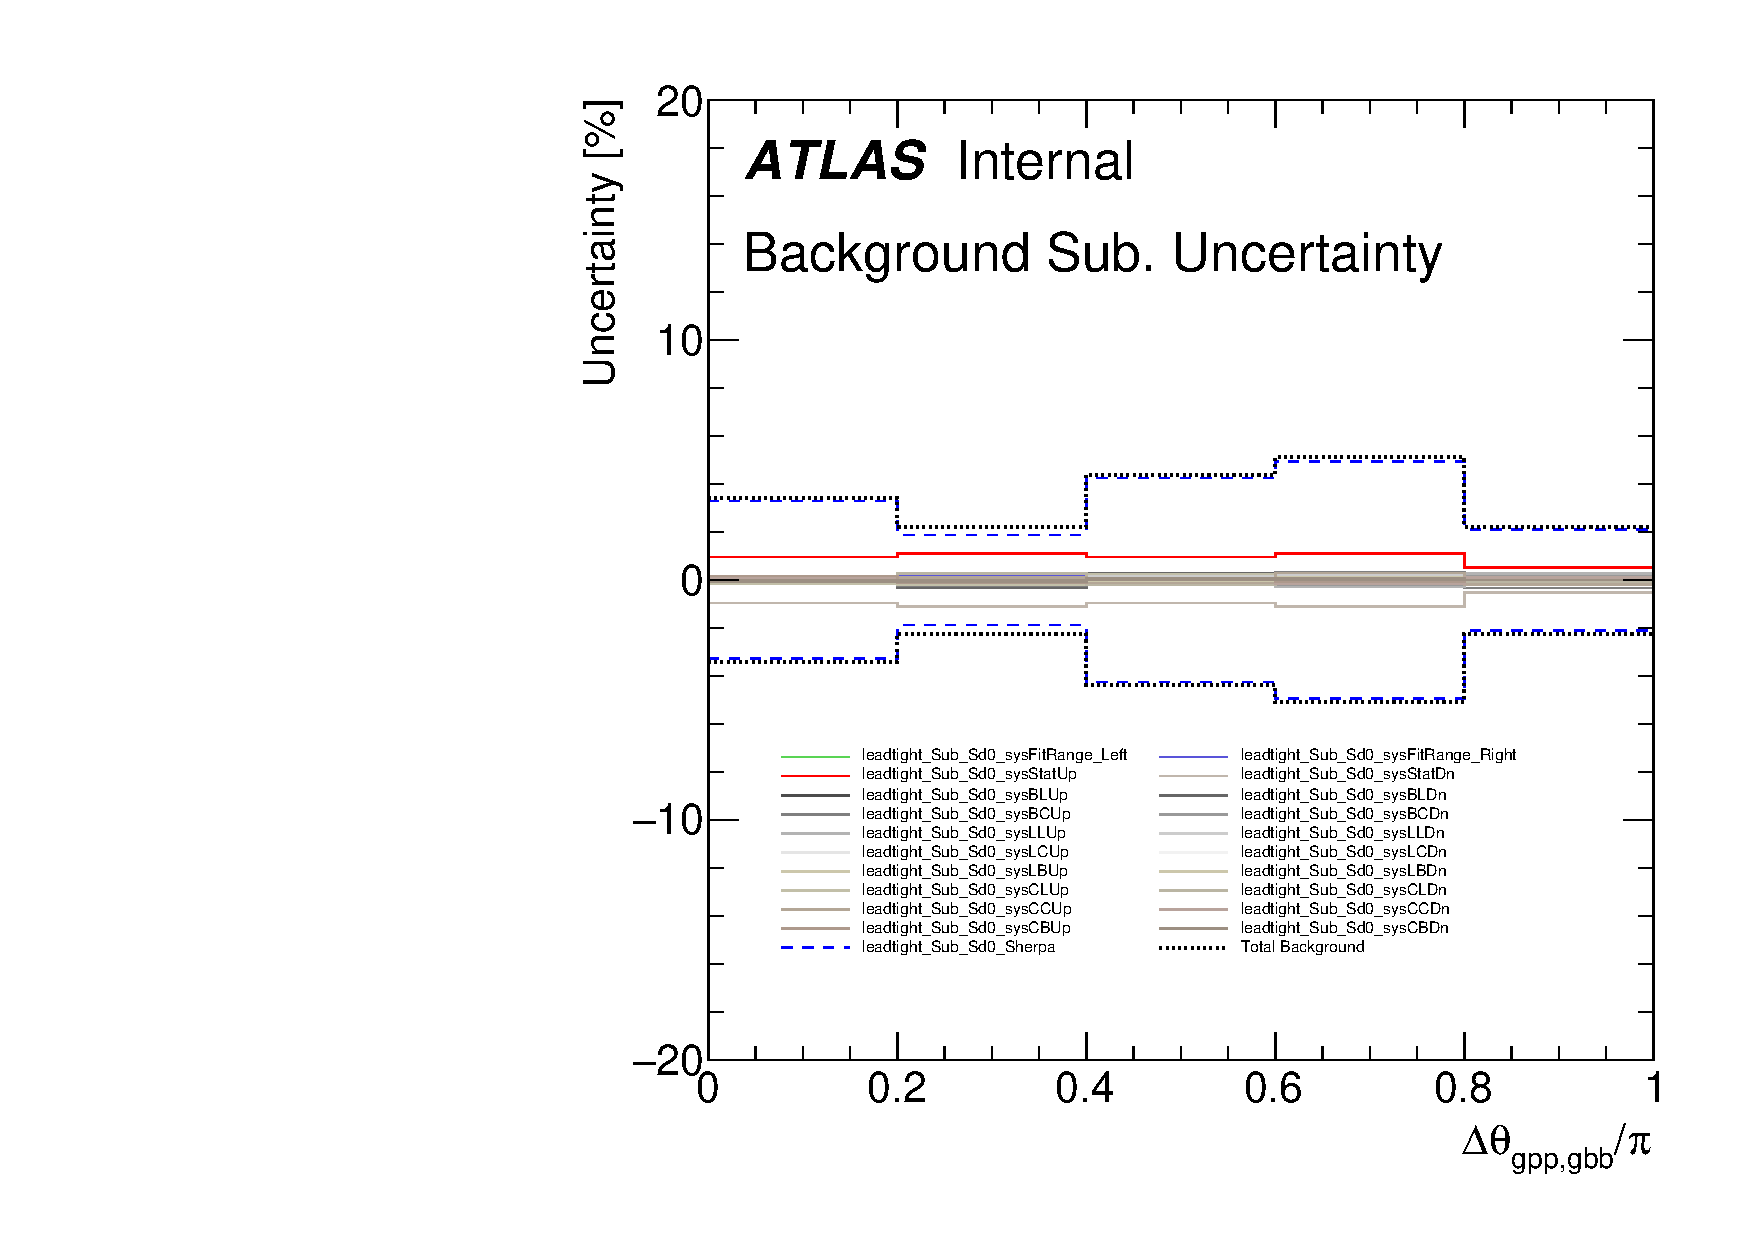
\includegraphics[width=0.45\linewidth]{figures/gbb/Unfolding/dphi2_uncert_summary.pdf}\\
%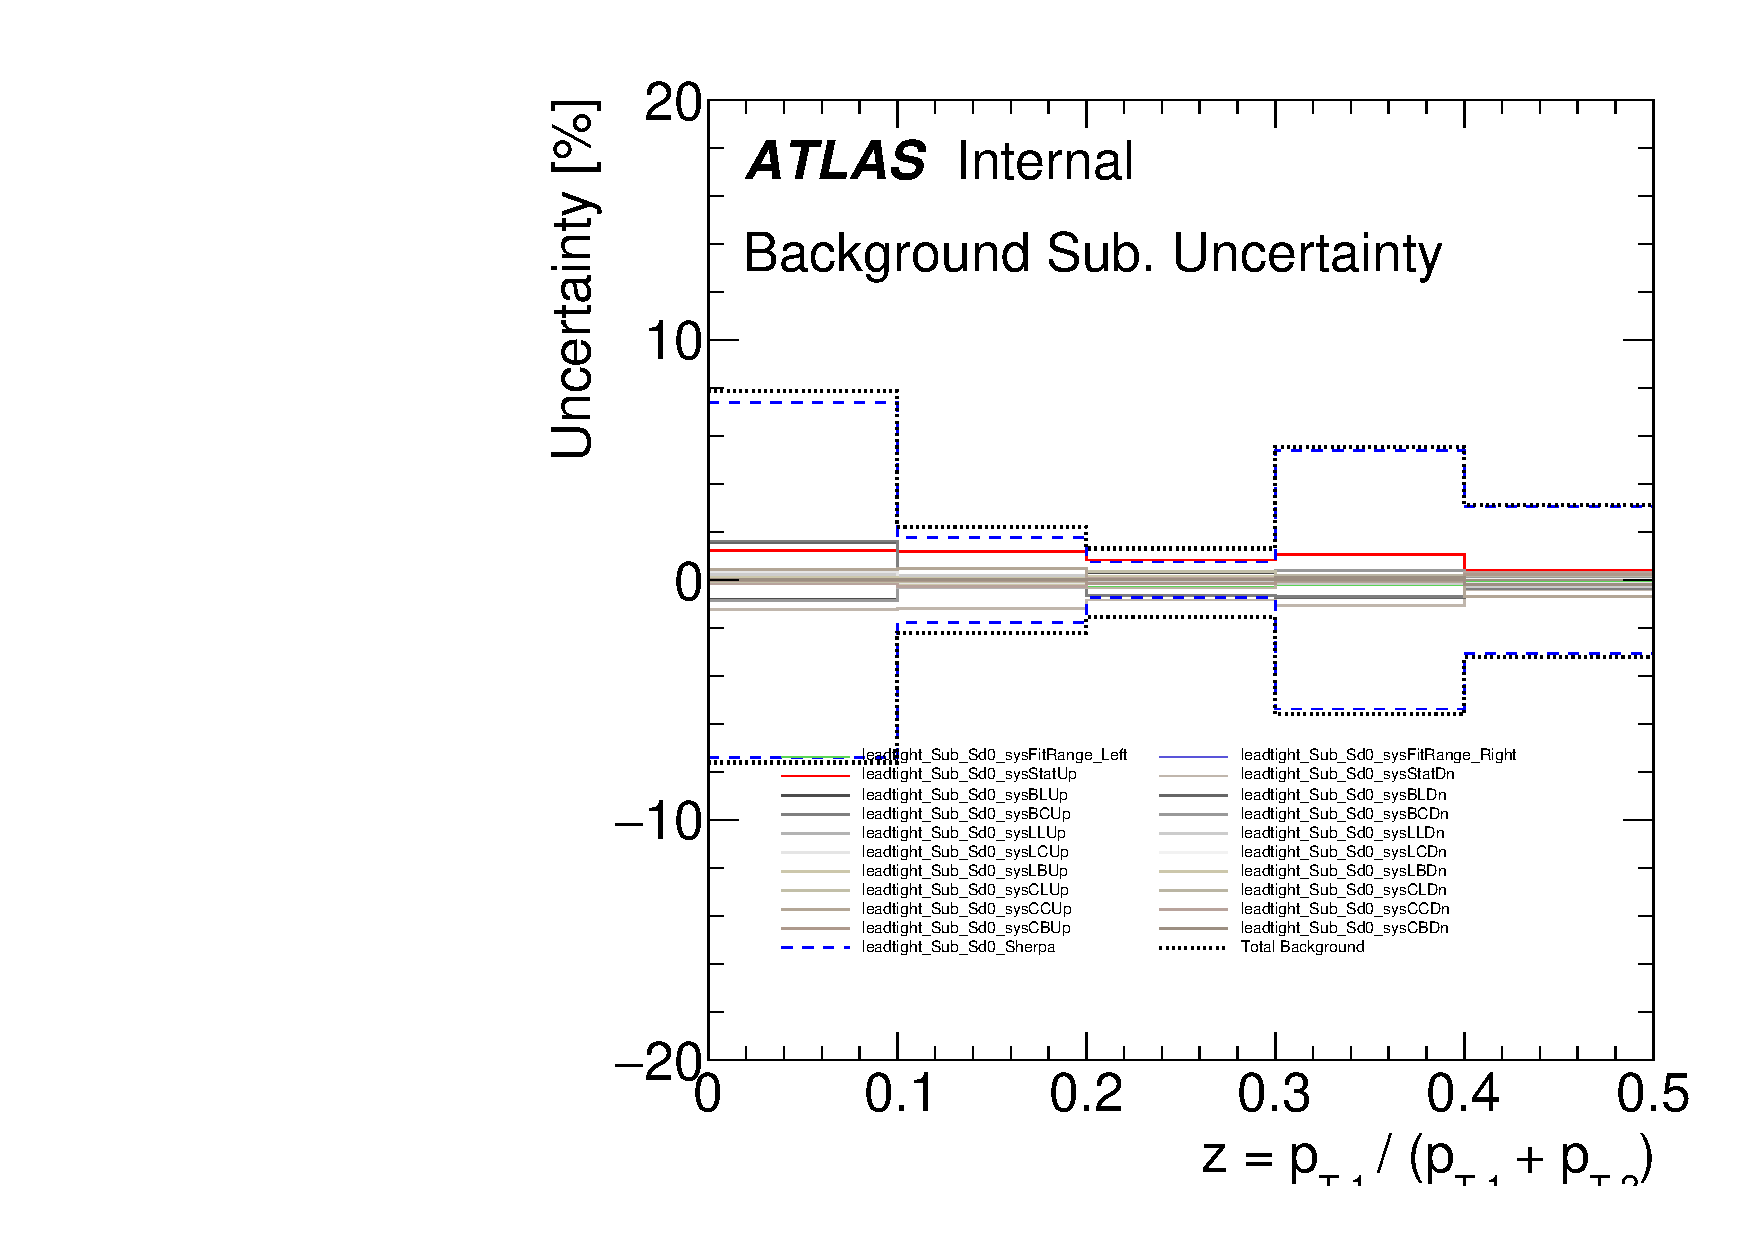
\includegraphics[width=0.45\linewidth]{figures/gbb/Unfolding/ZpT2_uncert_summary.pdf}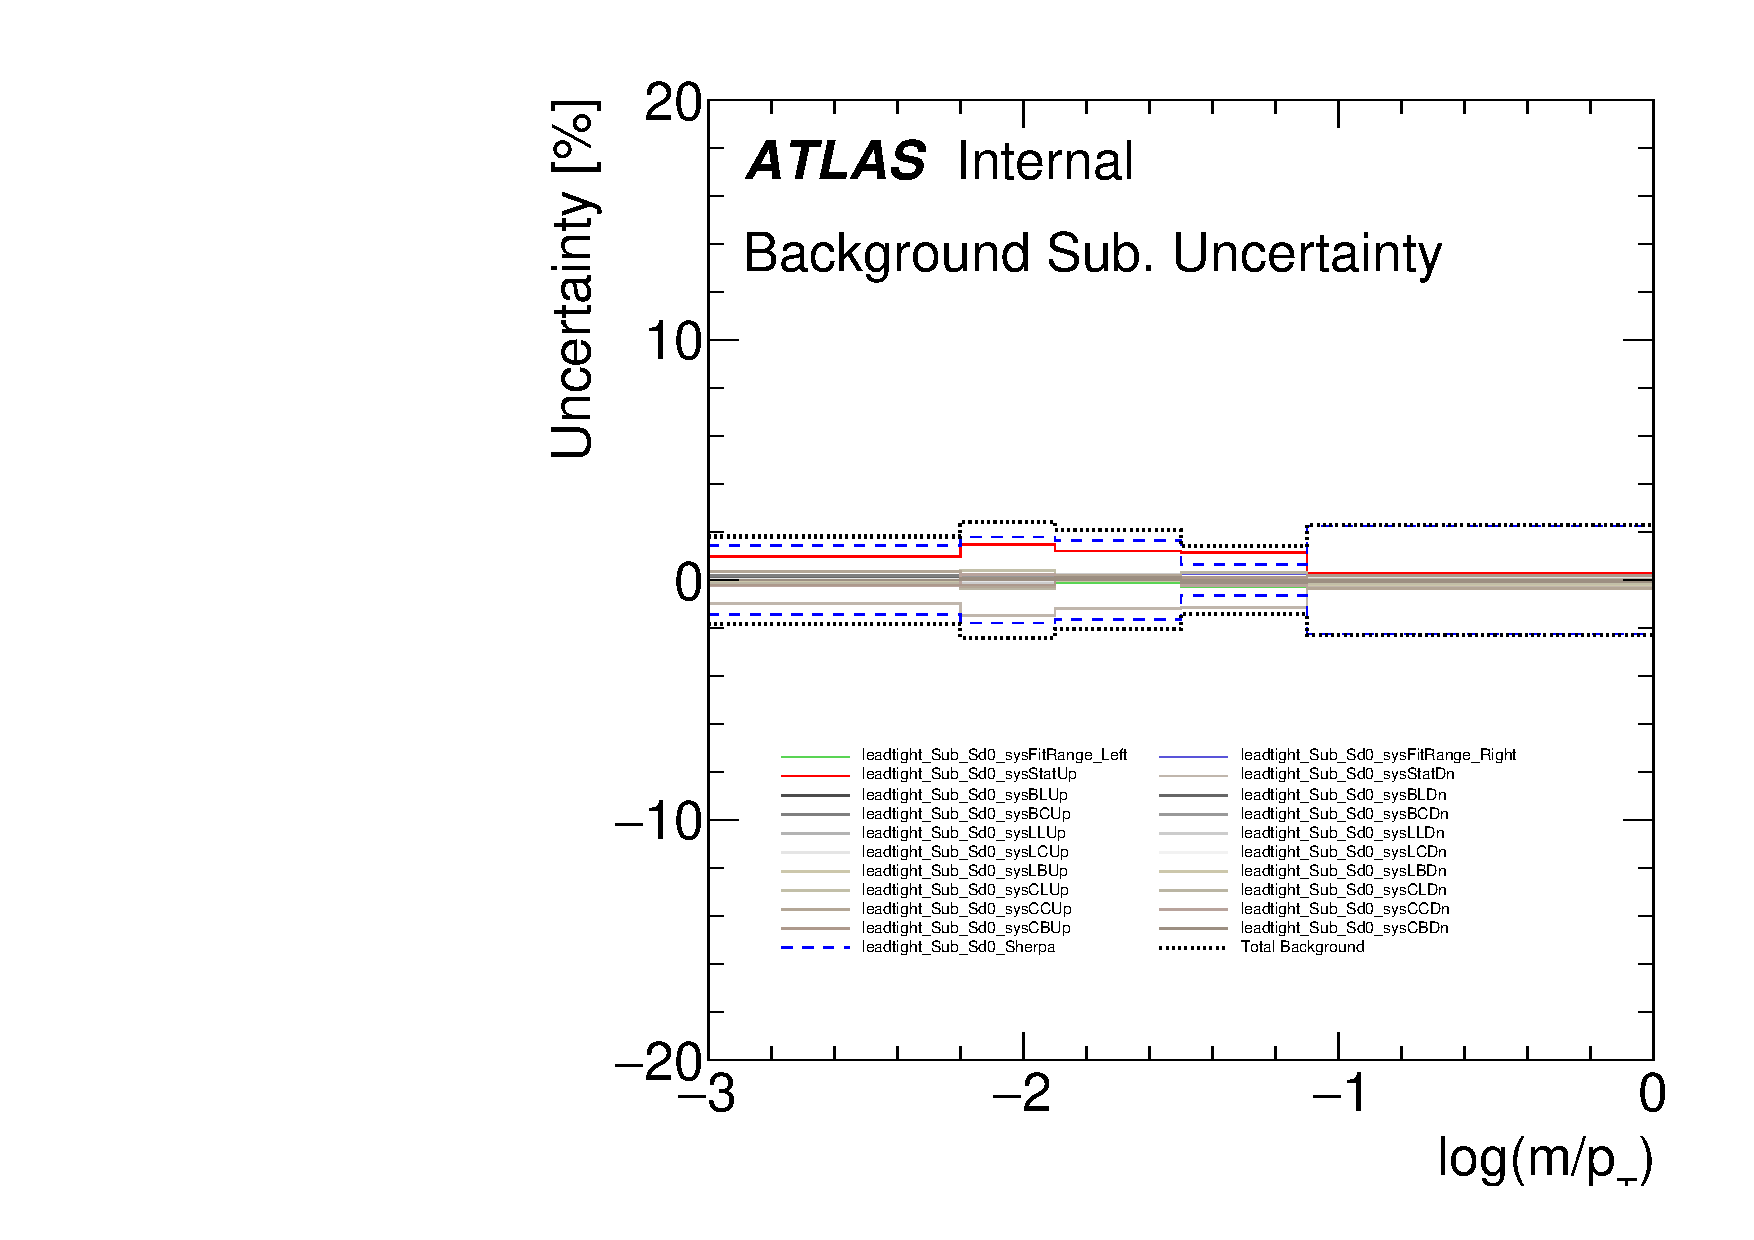
\includegraphics[width=0.45\linewidth]{figures/gbb/Unfolding/fracmasspt2_uncert_summary.pdf}
%\caption[]{A summary of the jet energy systematic uncertainties for all four observables. } 
%\label{fig:syst_overview_deltaR2}
%\end{center}
%\end{figure}

\subsection{Theoretical Systematic Uncertainties}
\label{sec:gbb-systs:theory}

The theoretical systematic uncertainty is taken two-fold. The prior difference between Sherpa and Pythia are taken care of in Sec.~\ref{sec:gbb-systs:unfolding}. The efficiency, fake factor and unfolding matrices difference summed in quadrature are taken to be the theoretical systematic uncertainty. It is noteworthy the agreement between data and Sherpa is closer or at least similar to that between data and Pythia for all unfolded distributions. But we do not use it as our nominal sample since statistics of Sherpa sample is two to eight times lower than that of Pythia.

%The unfolded result can depend on the modeling of jet fragmentation through the prior, the response matrix, and the correction factors.  Variations in the prior are already accounted for in the data-driven non-closure uncertainty from Sec.~\ref{sec:gbb-systs:unfolding}.  However, it is useful to examine the predictions from a different MC.  The particle-level distributions for Pythia and Sherpa are shown in Fig.~\ref{fig:frag1}.  There are significant differences between these models, especially for $\Delta\phi$ and the mass and to a lesser extent $\Delta R$ and $z$.  A comparison of the detector-level distributions, also with data appear in Fig.~\ref{fig:frag2}.   Sherpa provides a better description of the data; it is not used as baseline because the MC stats are lower.  The actual uncertainty associated to the jet fragmentation modeling is shown in Fig.~\ref{fig:syst_overview_deltaR2frag}.  The blue solid line compares Pythia with Sherpa with significant double-counting with the non-closure uncertainty.  The fake- (efficiency-)factor line uses Pythia with the fake- (efficiency-)factor replaced by the one from Sherpa.  Finally, the response matrix only line uses the Pythia response matrix, but re-weighted so that the particle-level projection is the Sherpa particle-level distribution.  The fragmentation modeling uncertainty is the sum in quadrature of these last three components.  Figure~\ref{fig:resultsvalidation3} compares the Pythia and Sherpa response matrices and shows that the truth-level re-weighting that makes the prior change does not change the response matrix (as desired).  The biggest source of uncertainty for the $\Delta\phi$ observable is from the response matrix in the first and last bins. This is because Pythia and Sherpa predict a different distribution for the leading and sub-leading track jets and thus the number of times that the angle is off by $\pi$ is different between the two.

%\textbf{Why doesn't Pythia have the same normalization as data?  }

%We compare Sherpa unfolded with Pythia with Sherpa truth.  There is some double-counting with the data-driven non-closure (Sec.~\ref{sec:gbb-systs:unfolding}).  The uncertainty breakdown is shown in Fig.~\ref{fig:syst_overview_deltaR2frag}.  

%\begin{figure}[htpb!]
%\begin{center}
%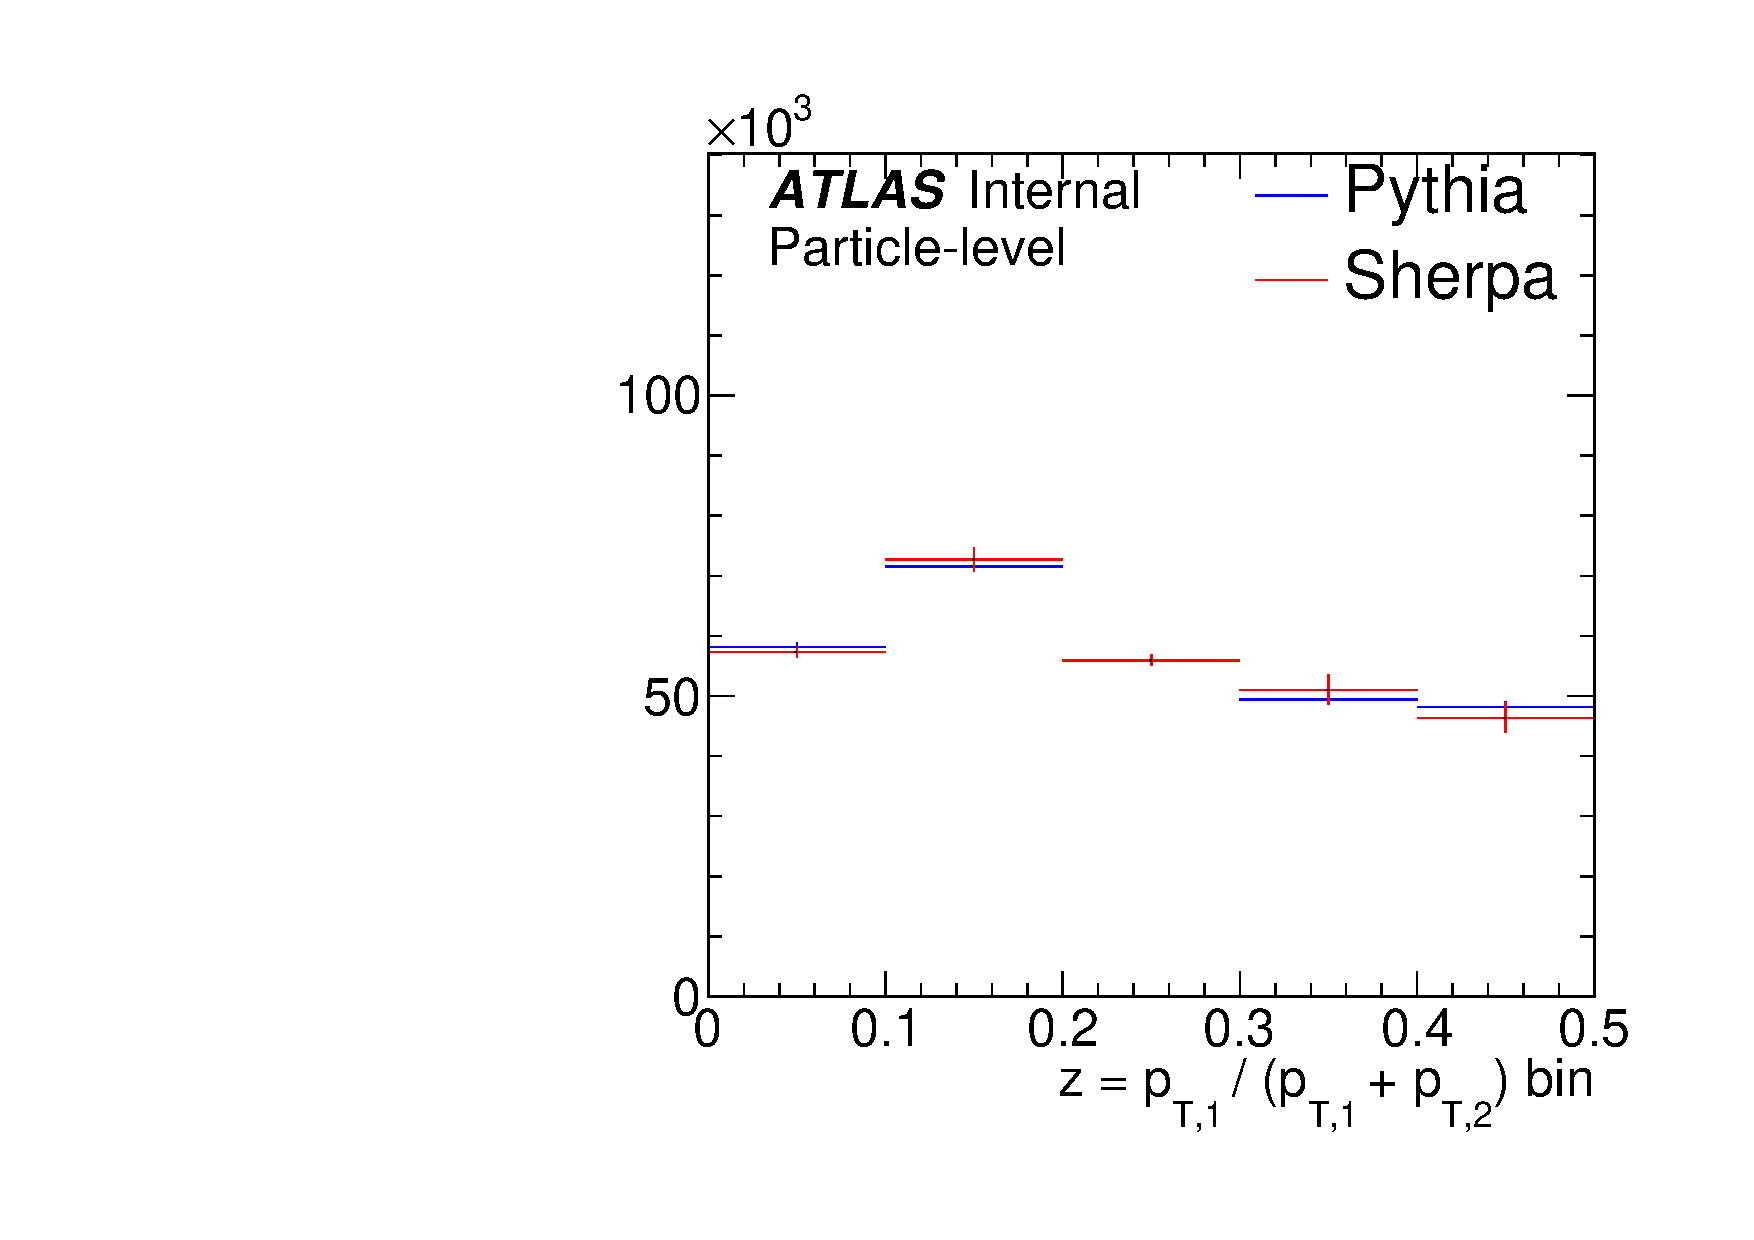
\includegraphics[width=0.45\linewidth]{figures/gbb/Unfolding/PythiavsSherpaTruthZpT.pdf}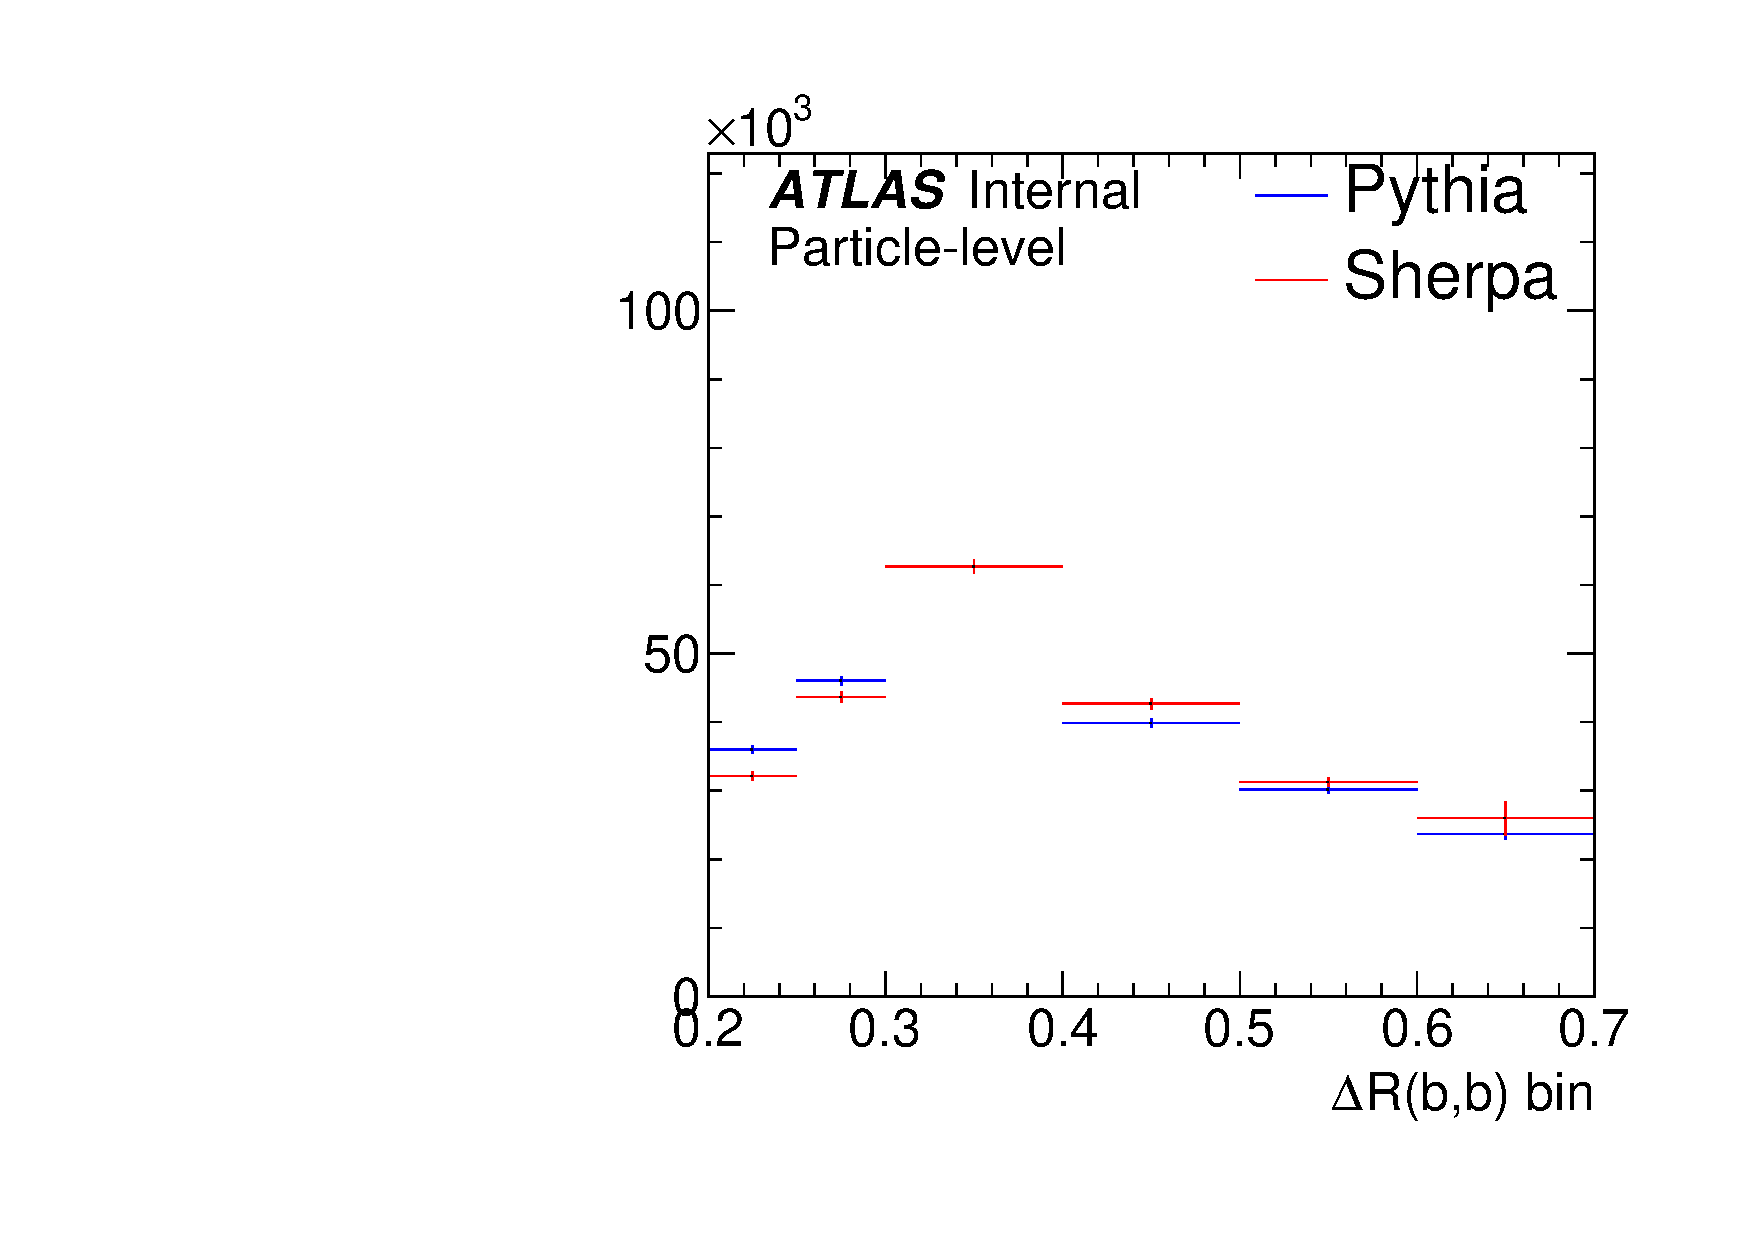
\includegraphics[width=0.45\linewidth]{figures/gbb/Unfolding/PythiavsSherpaTruthdR.pdf}\\
%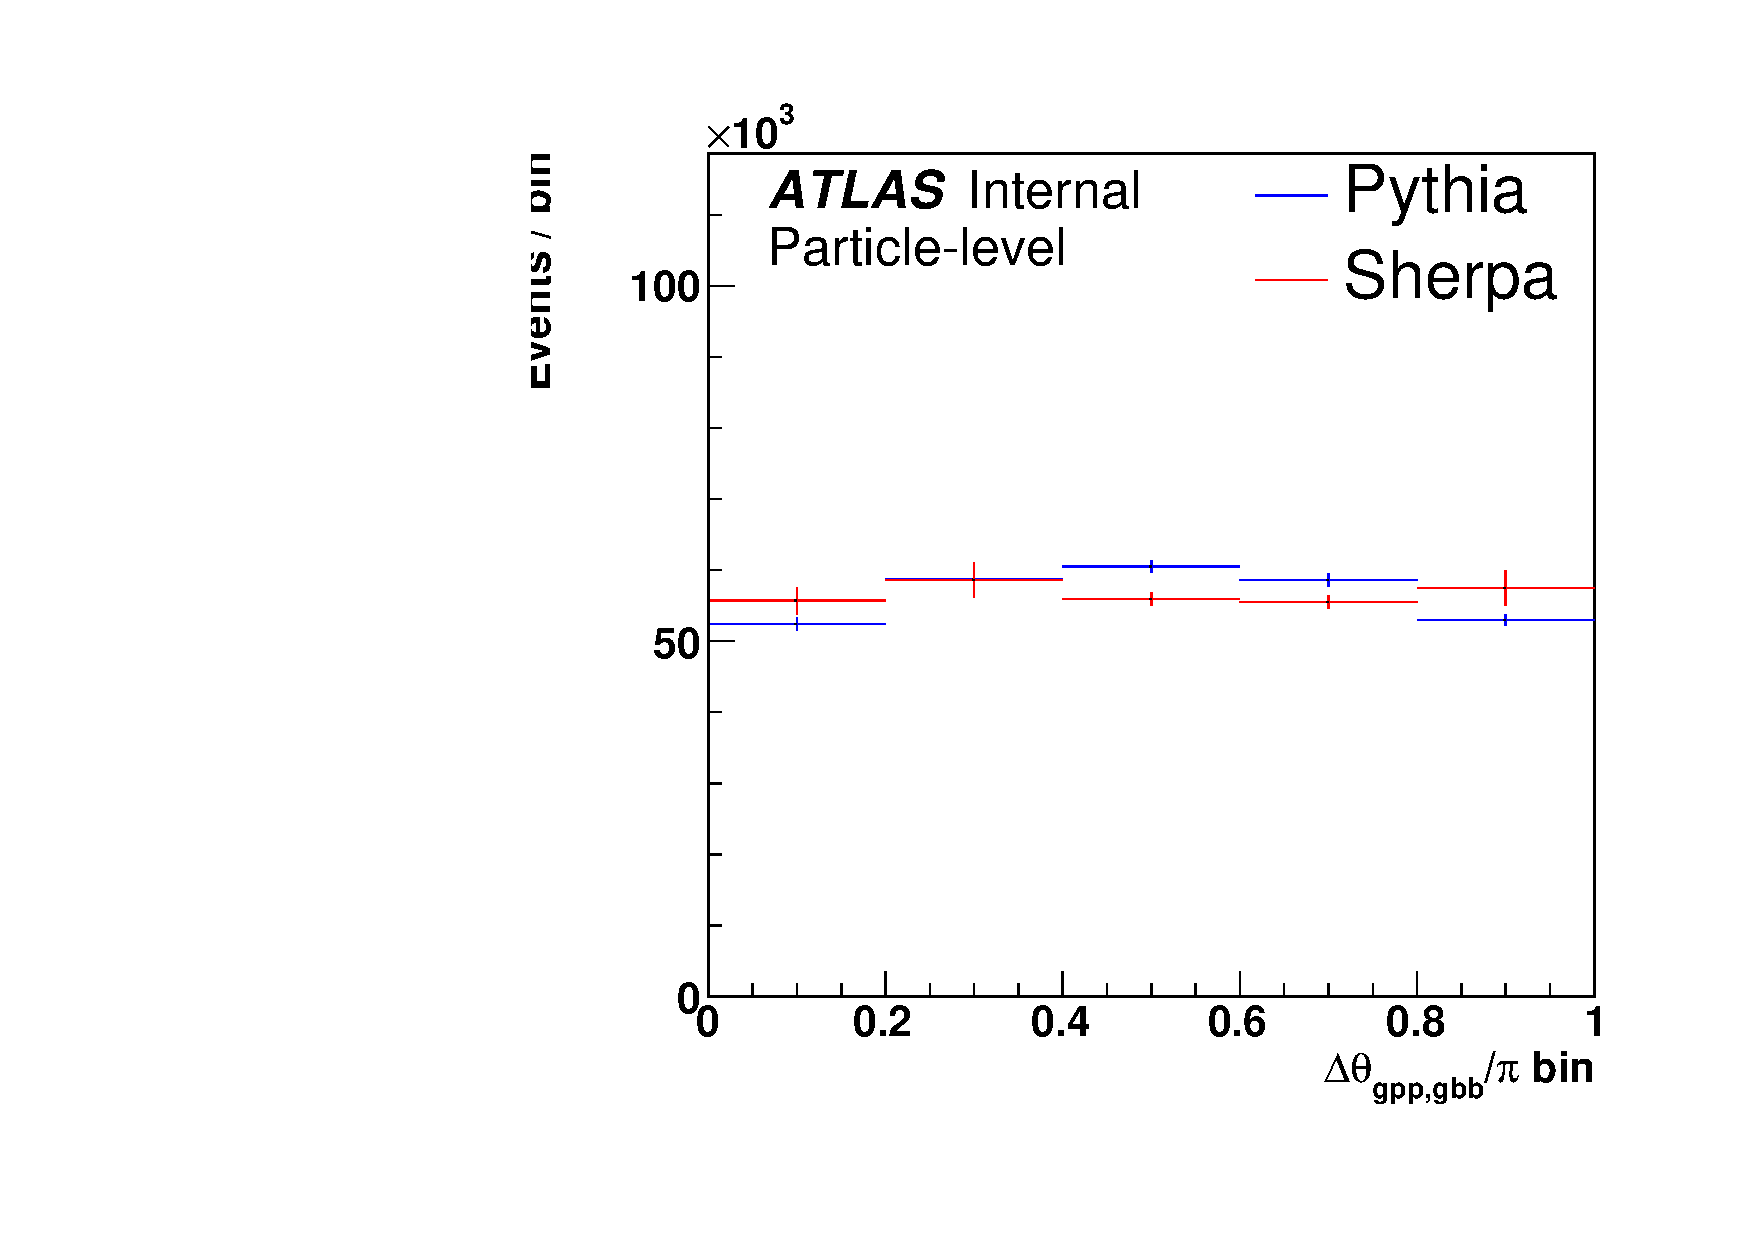
\includegraphics[width=0.45\linewidth]{figures/gbb/Unfolding/PythiavsSherpaTruthdphi.pdf}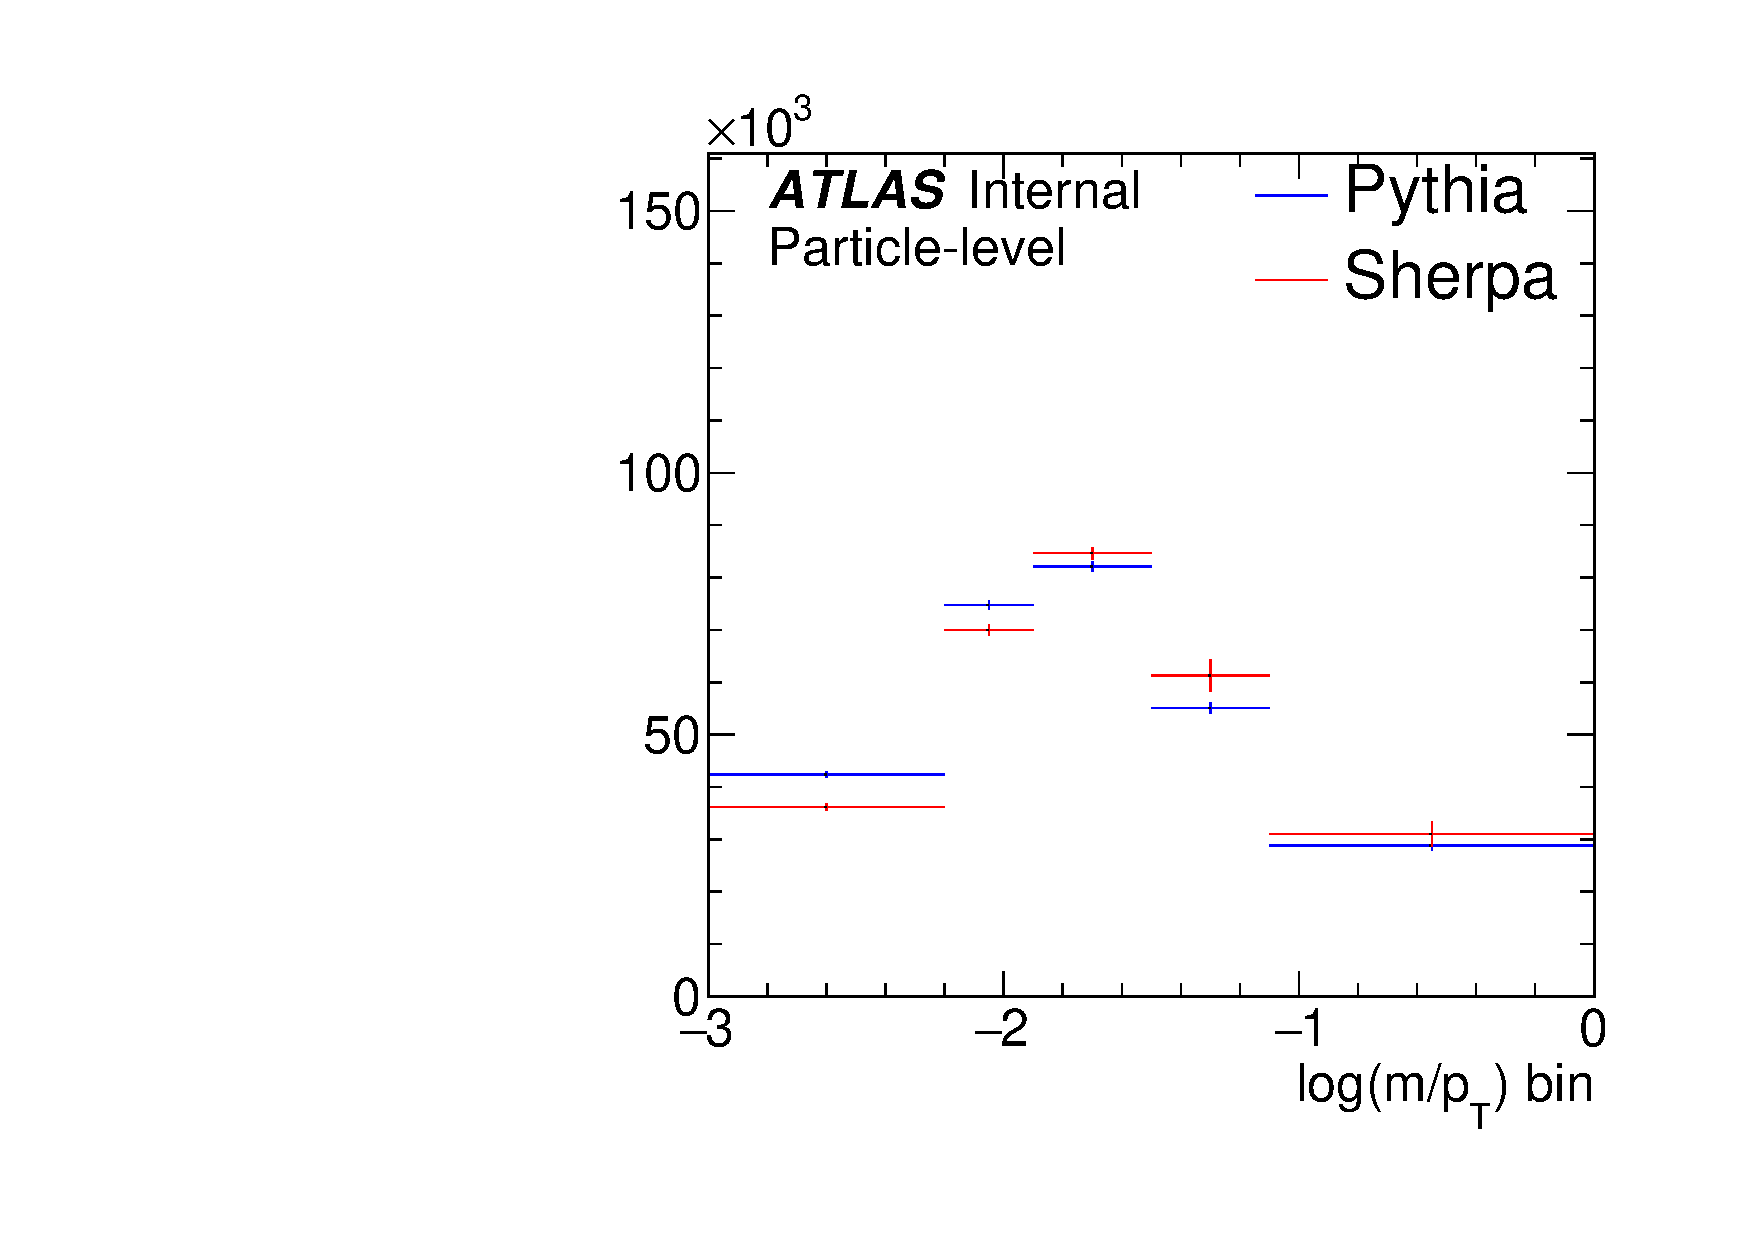
\includegraphics[width=0.45\linewidth]{figures/gbb/Unfolding/PythiavsSherpaTruthfracmasspt.pdf}
%\caption[]{A particle-level comparison between Pythia and Sherpa, where Sherpa is normalized to Pythia.} 
%\label{fig:frag1}
%\end{center}
%\end{figure}
%
%\begin{figure}[htpb!]
%\begin{center}
%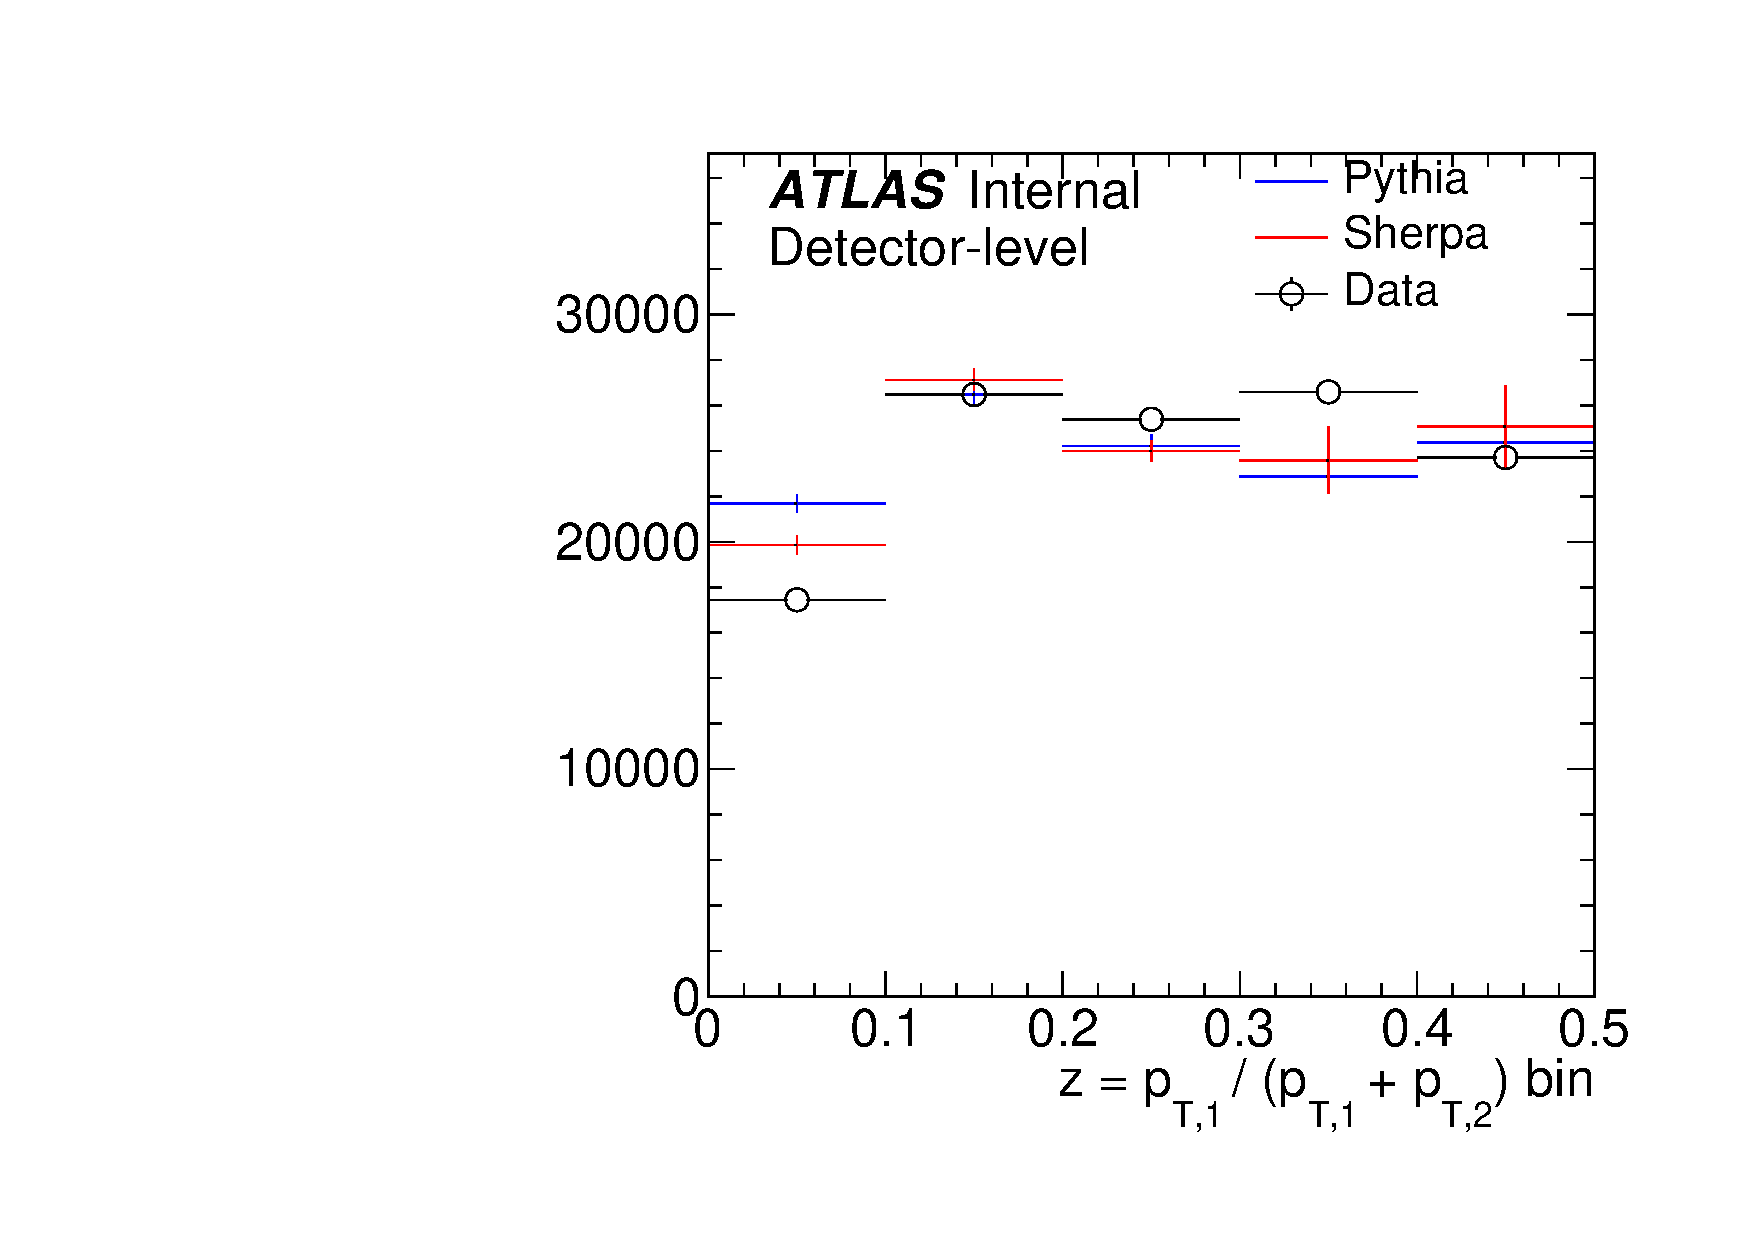
\includegraphics[width=0.45\linewidth]{figures/gbb/Unfolding/PythiavsSherpavsDataZpT.pdf}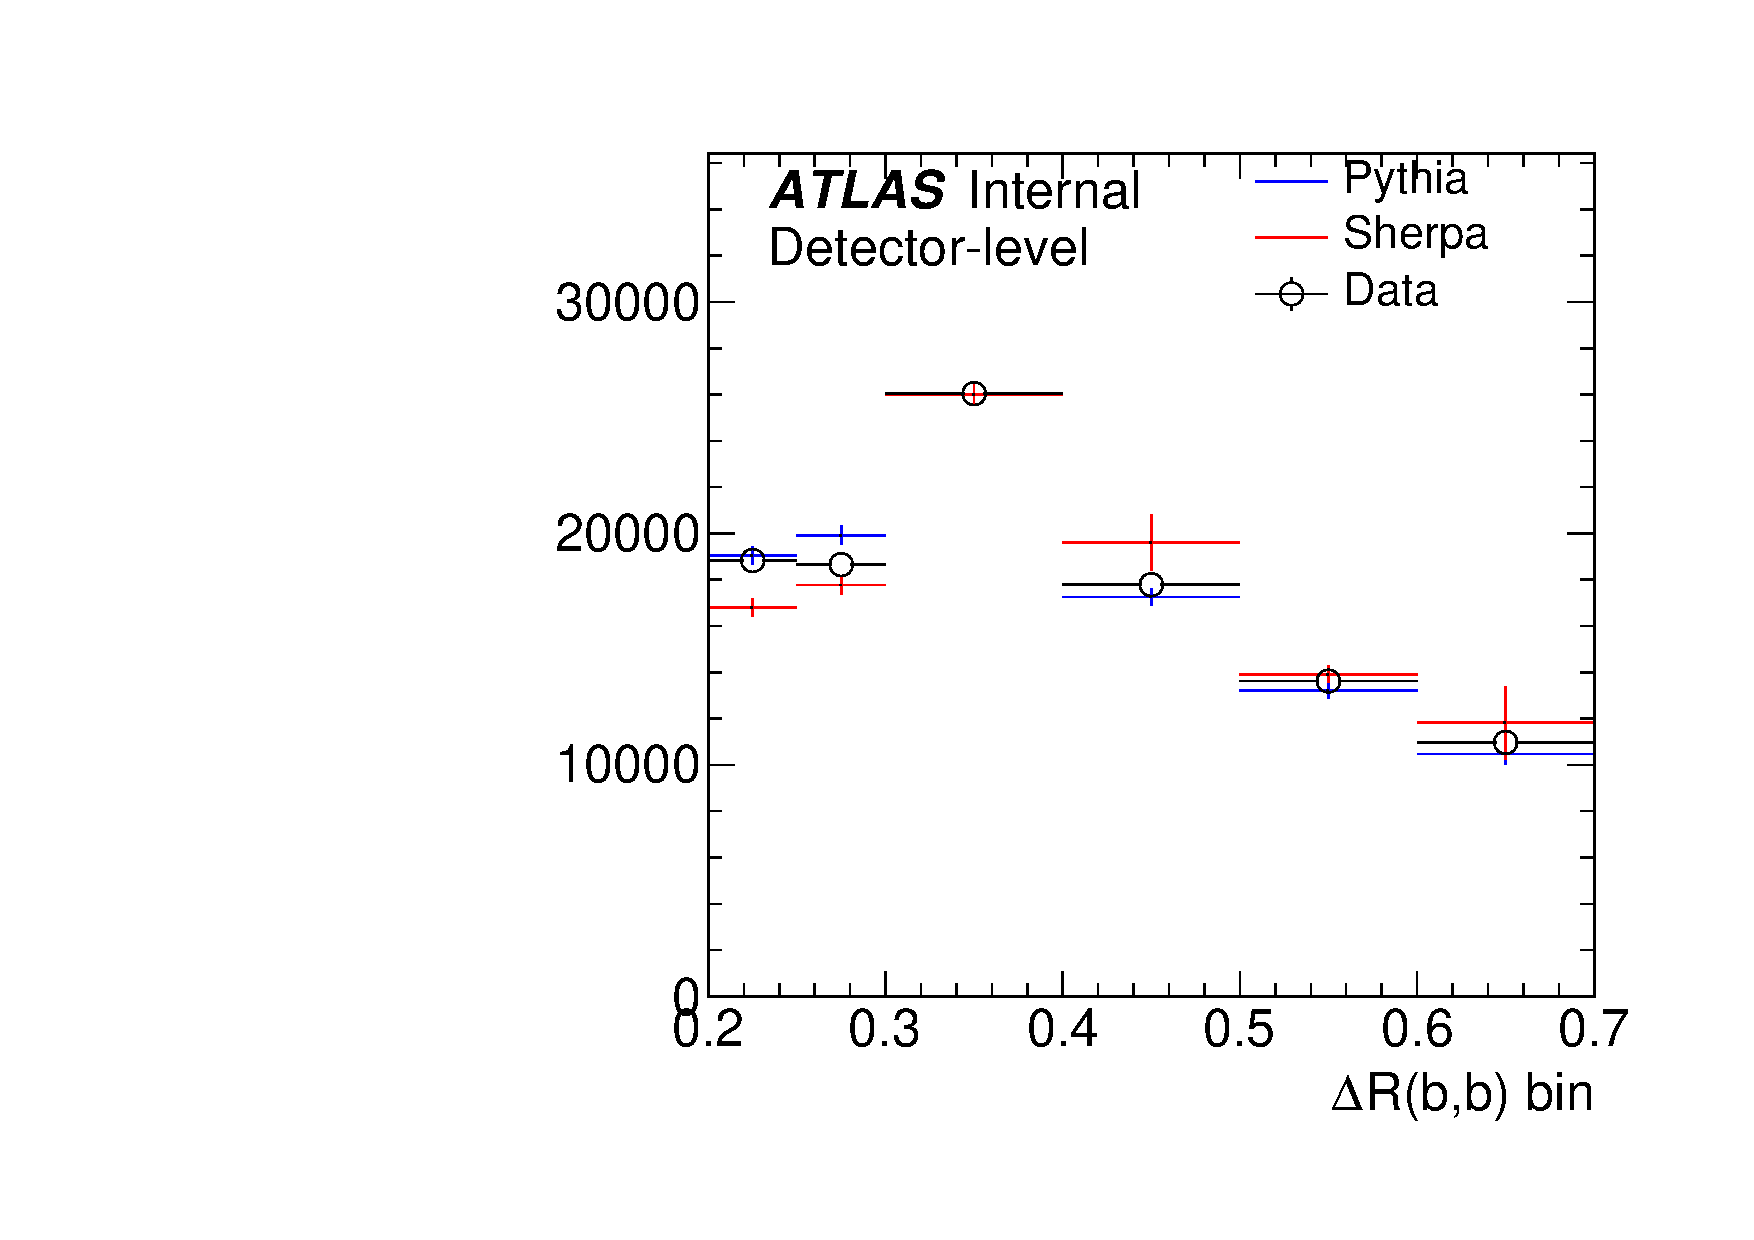
\includegraphics[width=0.45\linewidth]{figures/gbb/Unfolding/PythiavsSherpavsDatadR.pdf}\\
%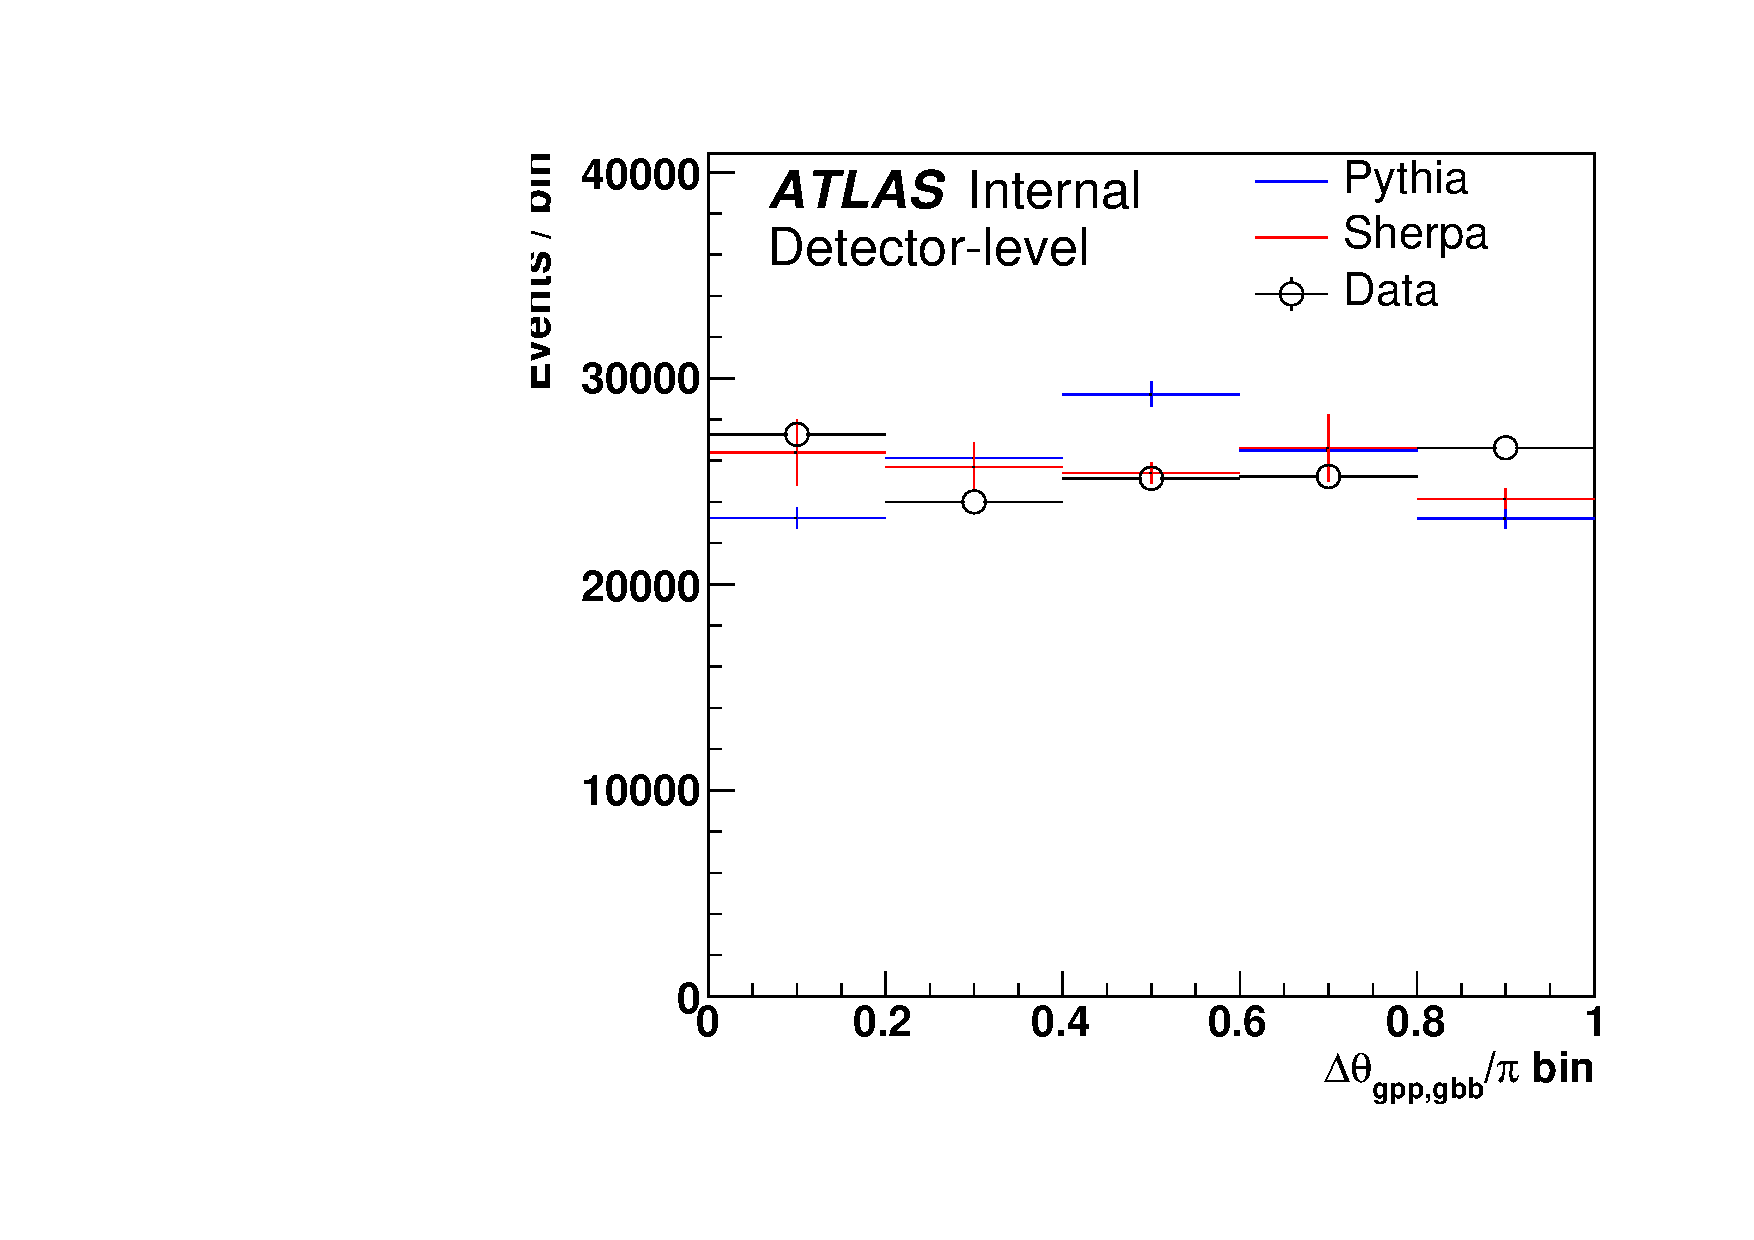
\includegraphics[width=0.45\linewidth]{figures/gbb/Unfolding/PythiavsSherpavsDatadphi.pdf}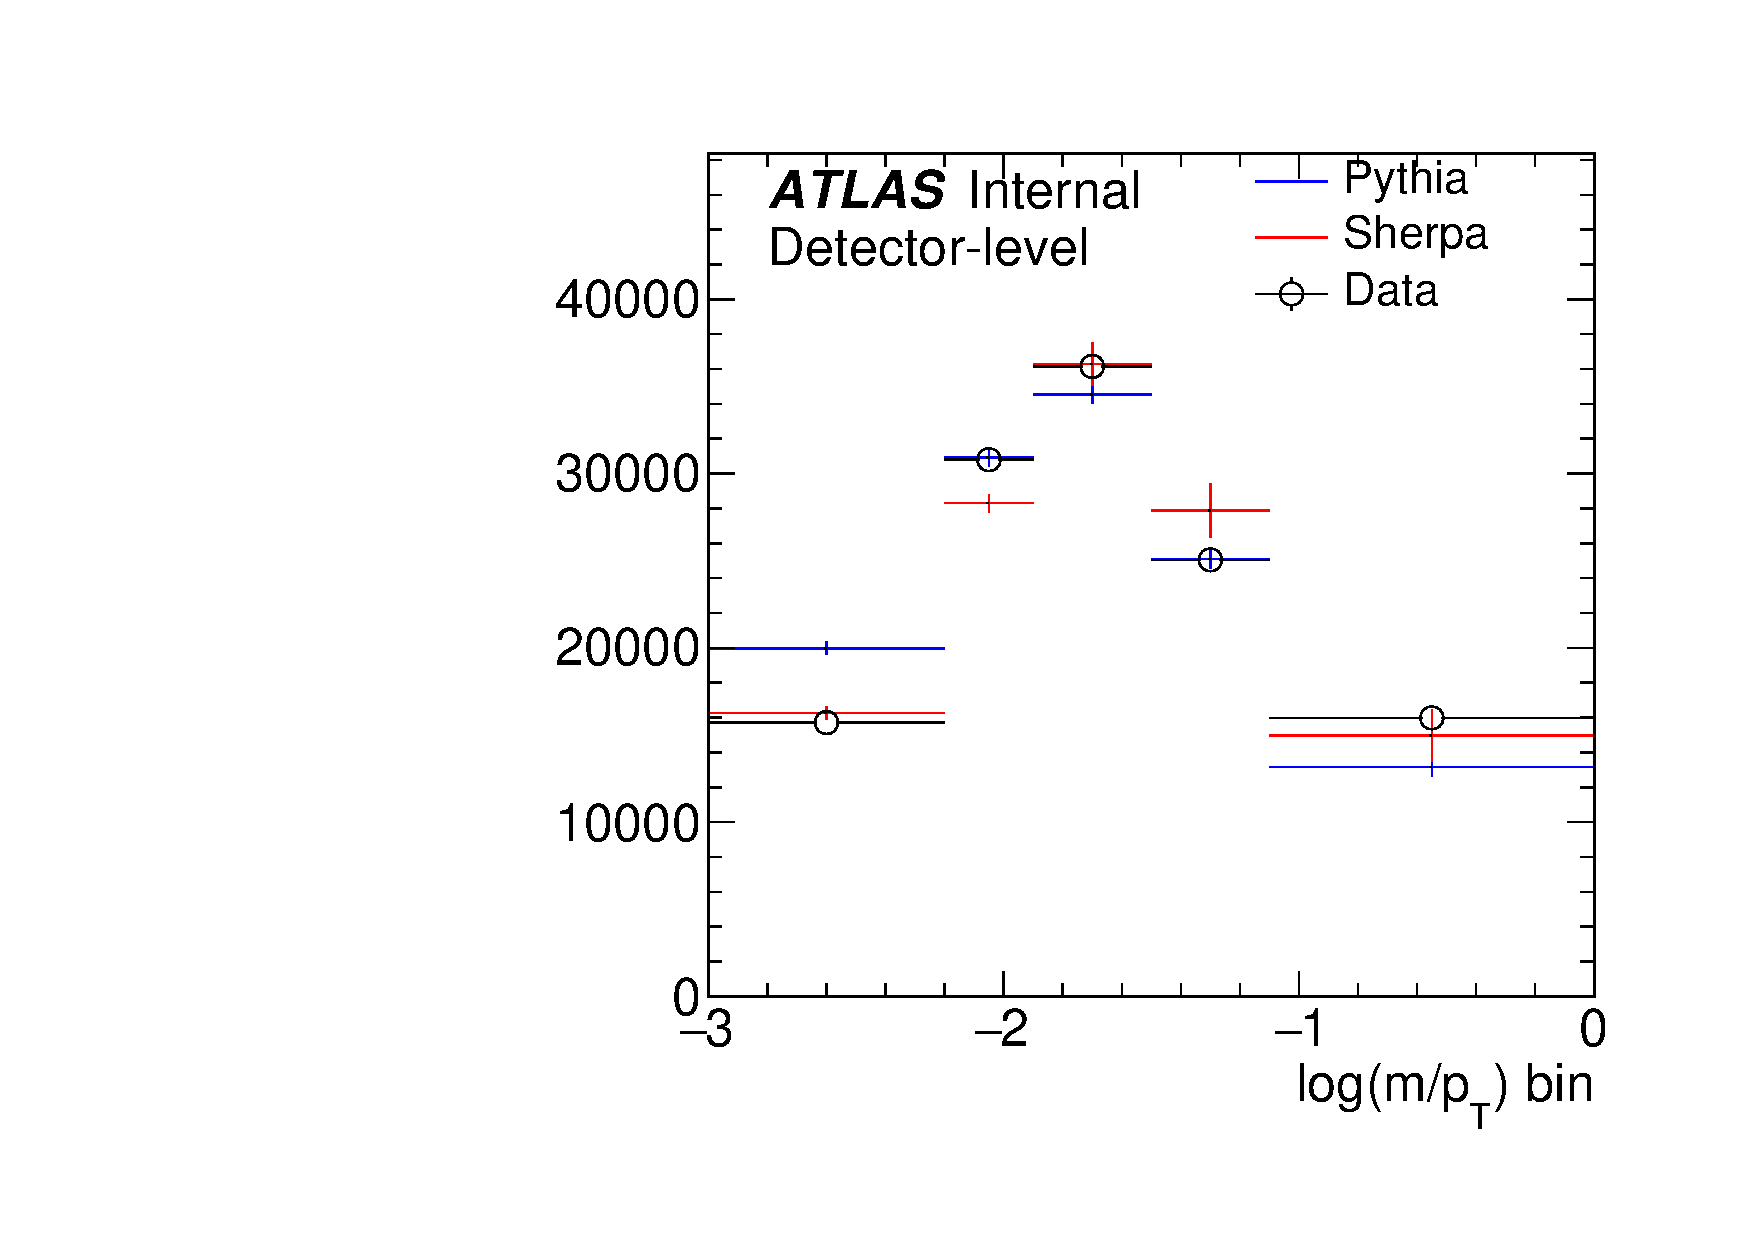
\includegraphics[width=0.45\linewidth]{figures/gbb/Unfolding/PythiavsSherpavsDatafracmasspt.pdf}
%\caption[]{A detector-level comparison between Pythia, Sherpa, and data.  The MC is normalized to the data.} 
%\label{fig:frag2}
%\end{center}
%\end{figure}
%  
%  \begin{figure}[htpb!]
%\begin{center}
%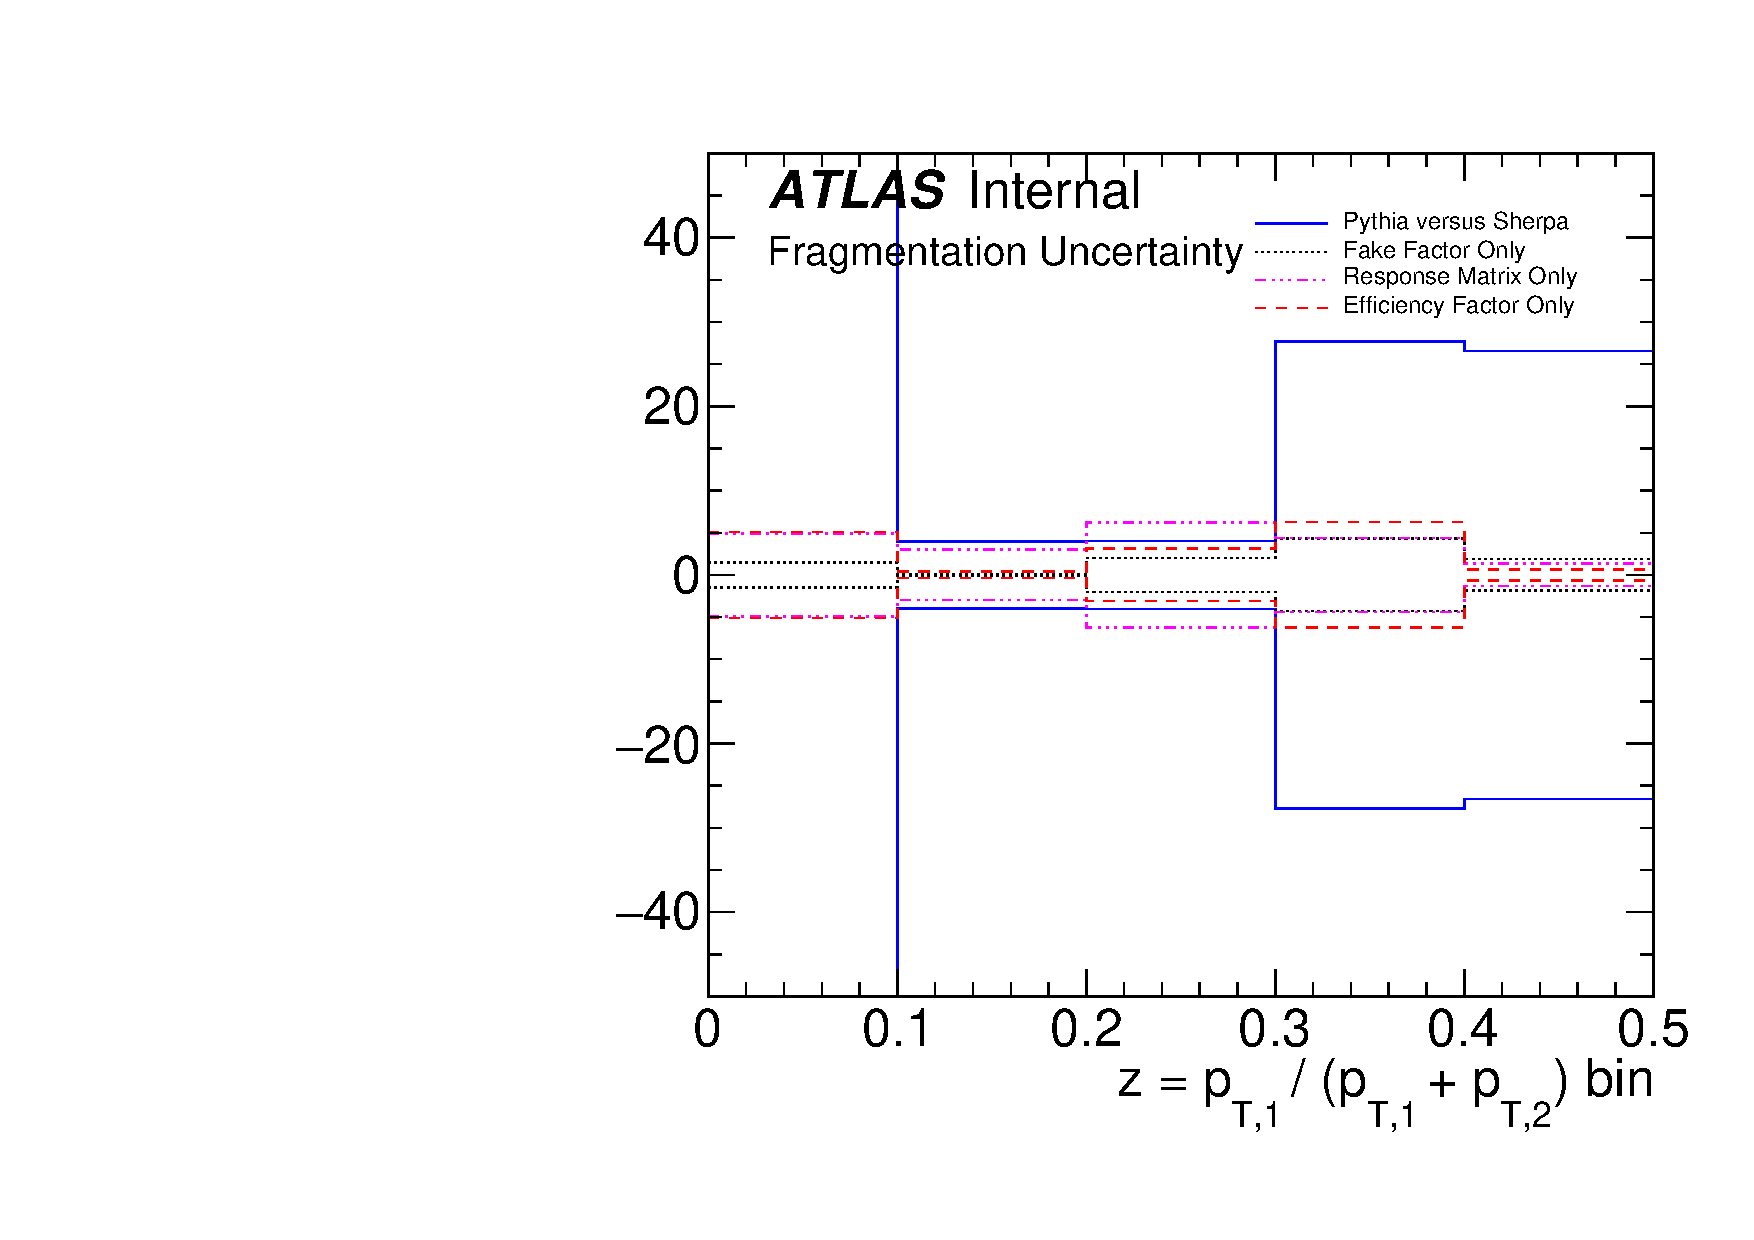
\includegraphics[width=0.45\linewidth]{figures/gbb/Unfolding/ZpT0_uncert_summary.pdf}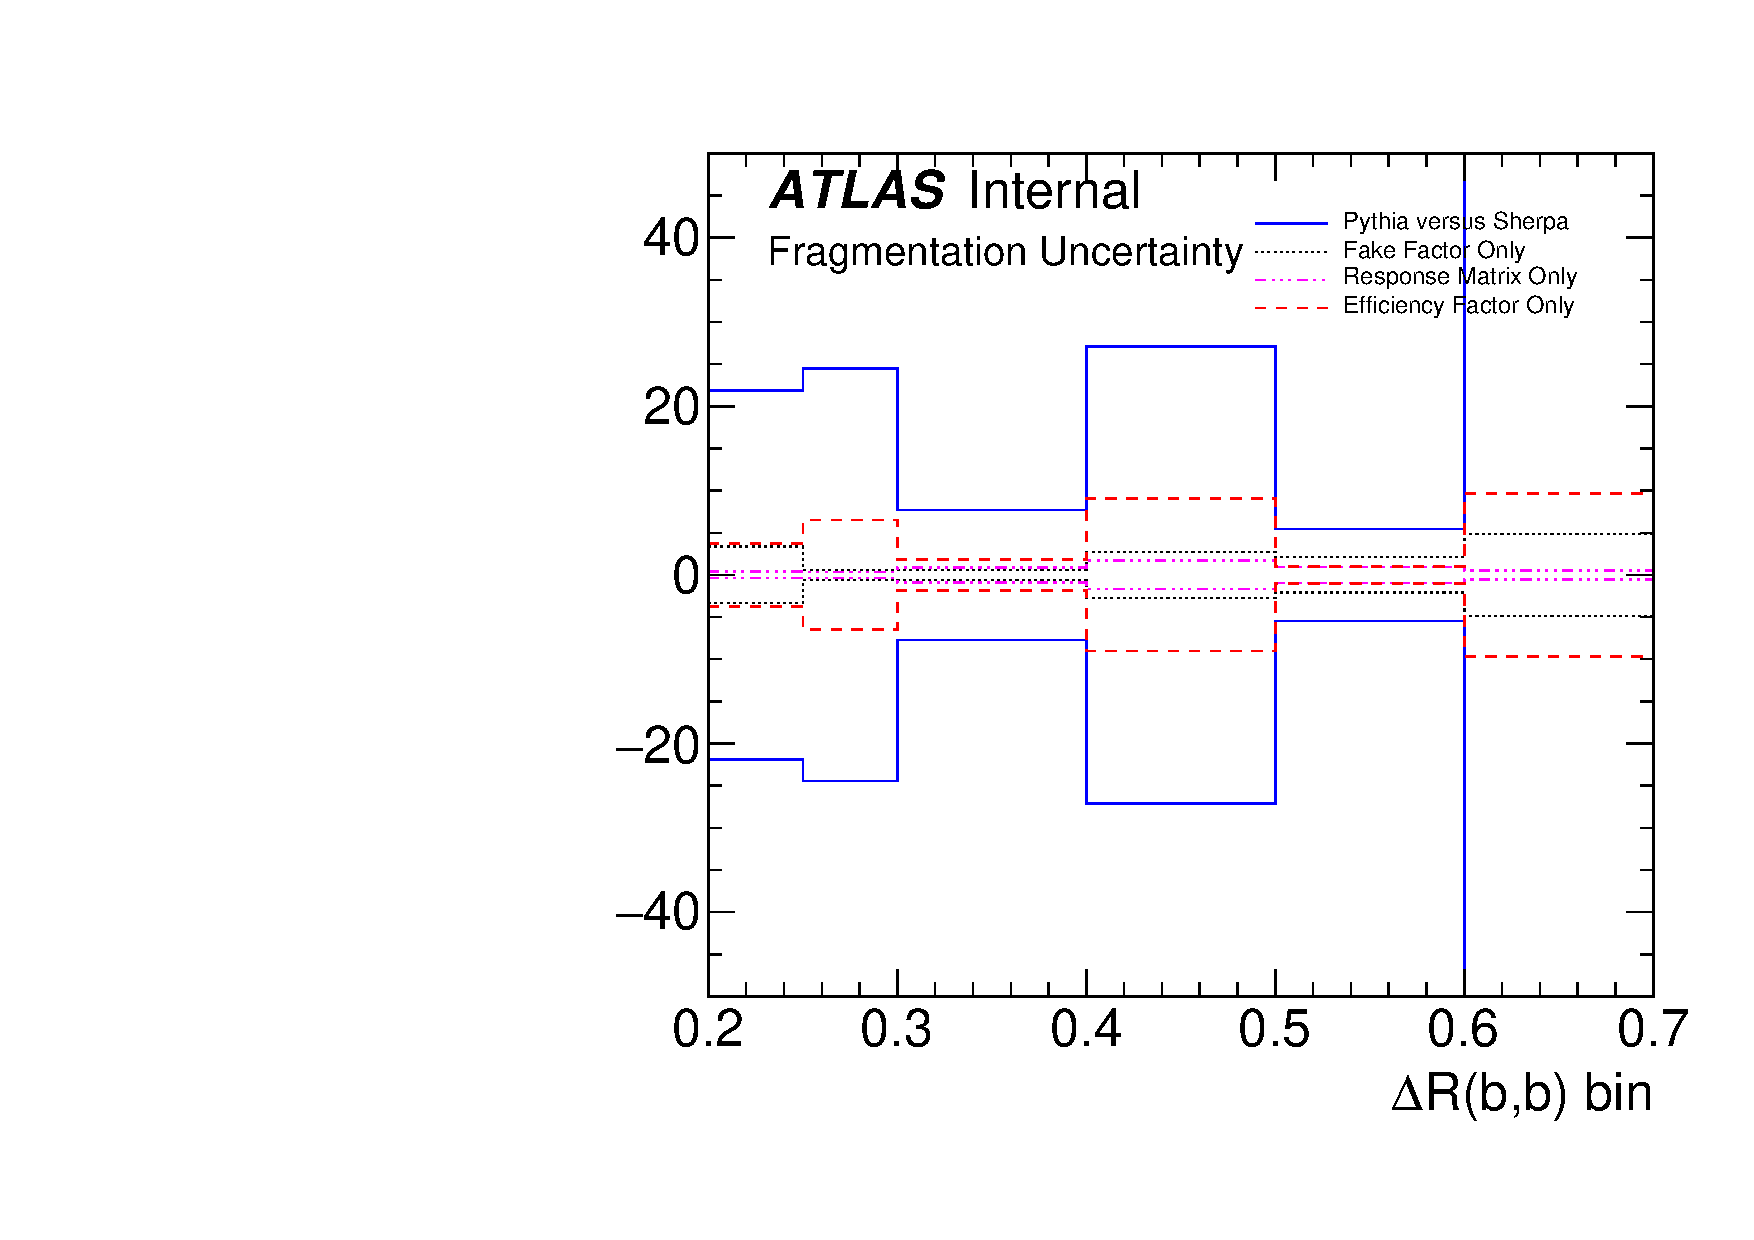
\includegraphics[width=0.45\linewidth]{figures/gbb/Unfolding/dR0_uncert_summary.pdf}\\
%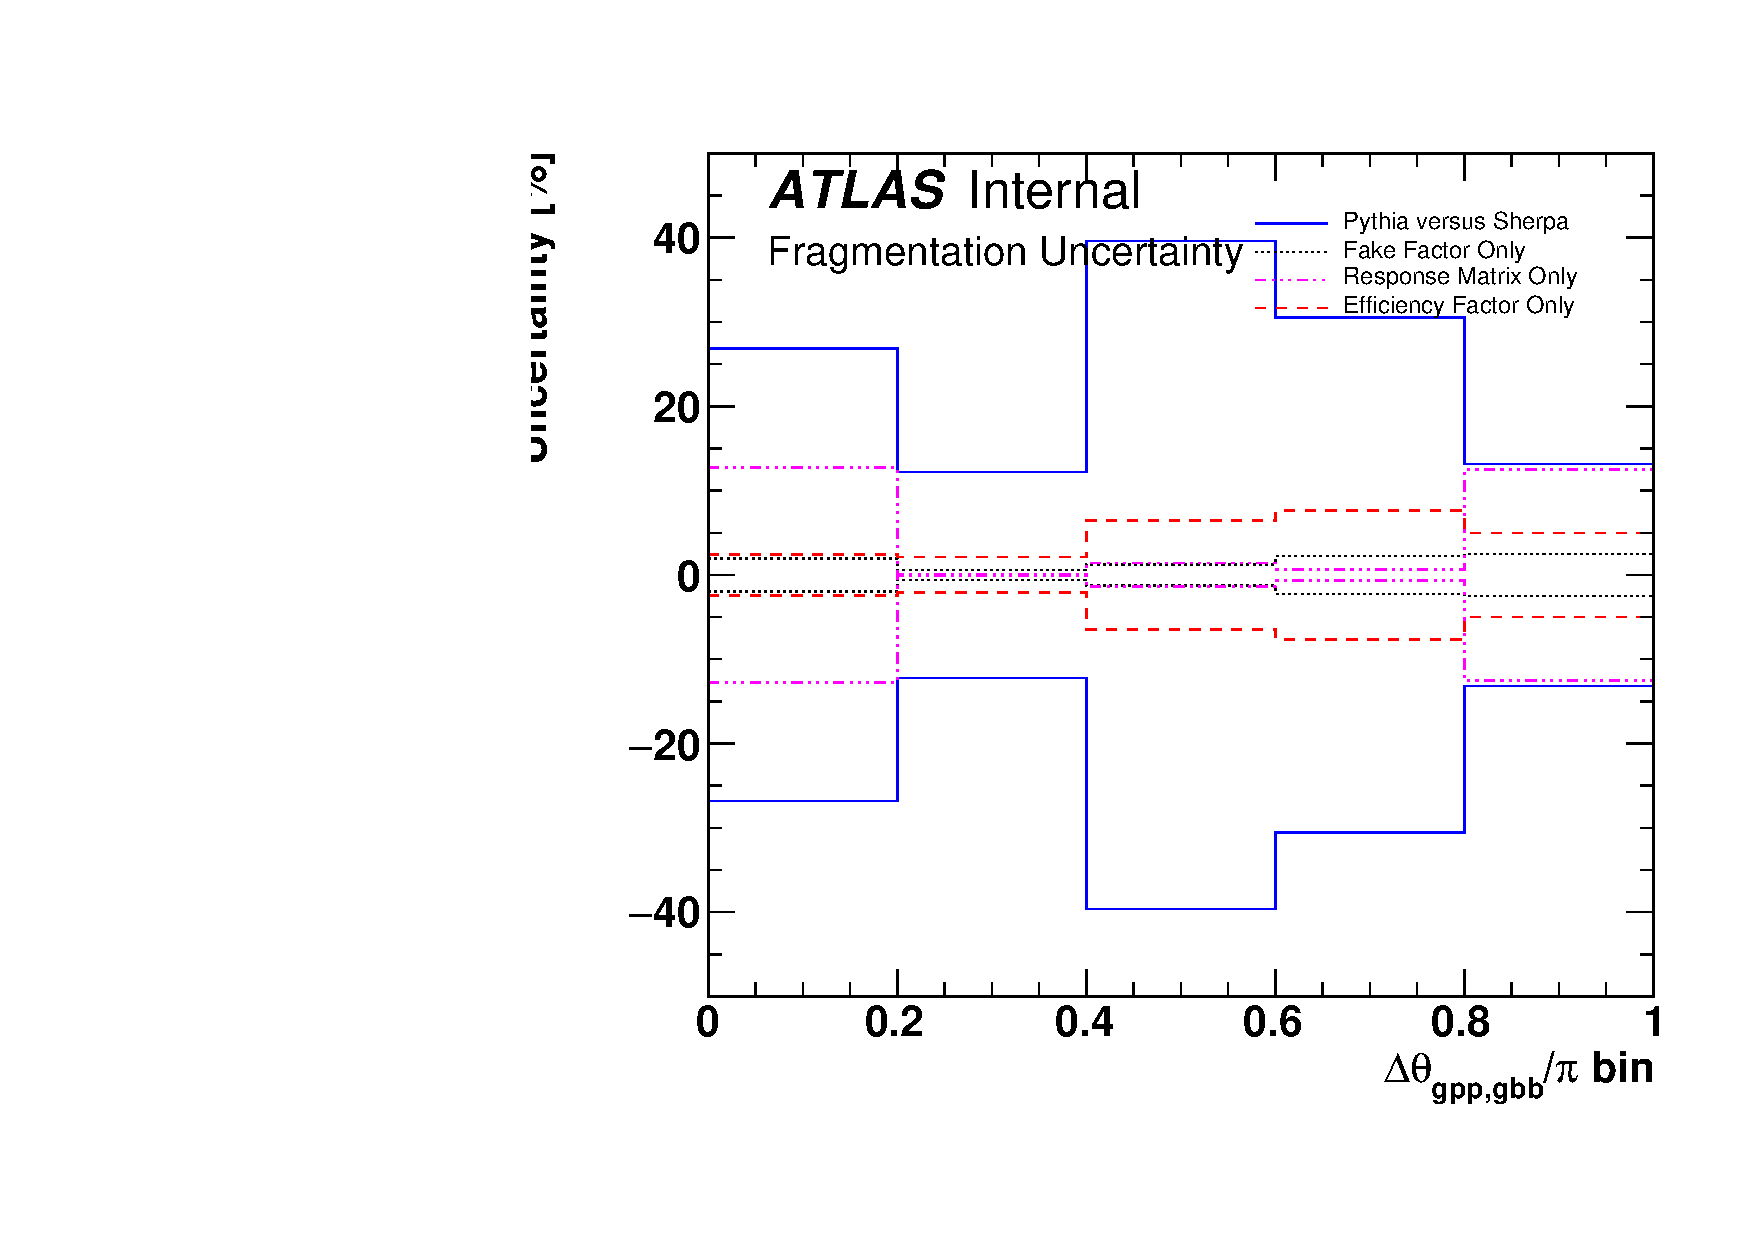
\includegraphics[width=0.45\linewidth]{figures/gbb/Unfolding/dphi0_uncert_summary.pdf}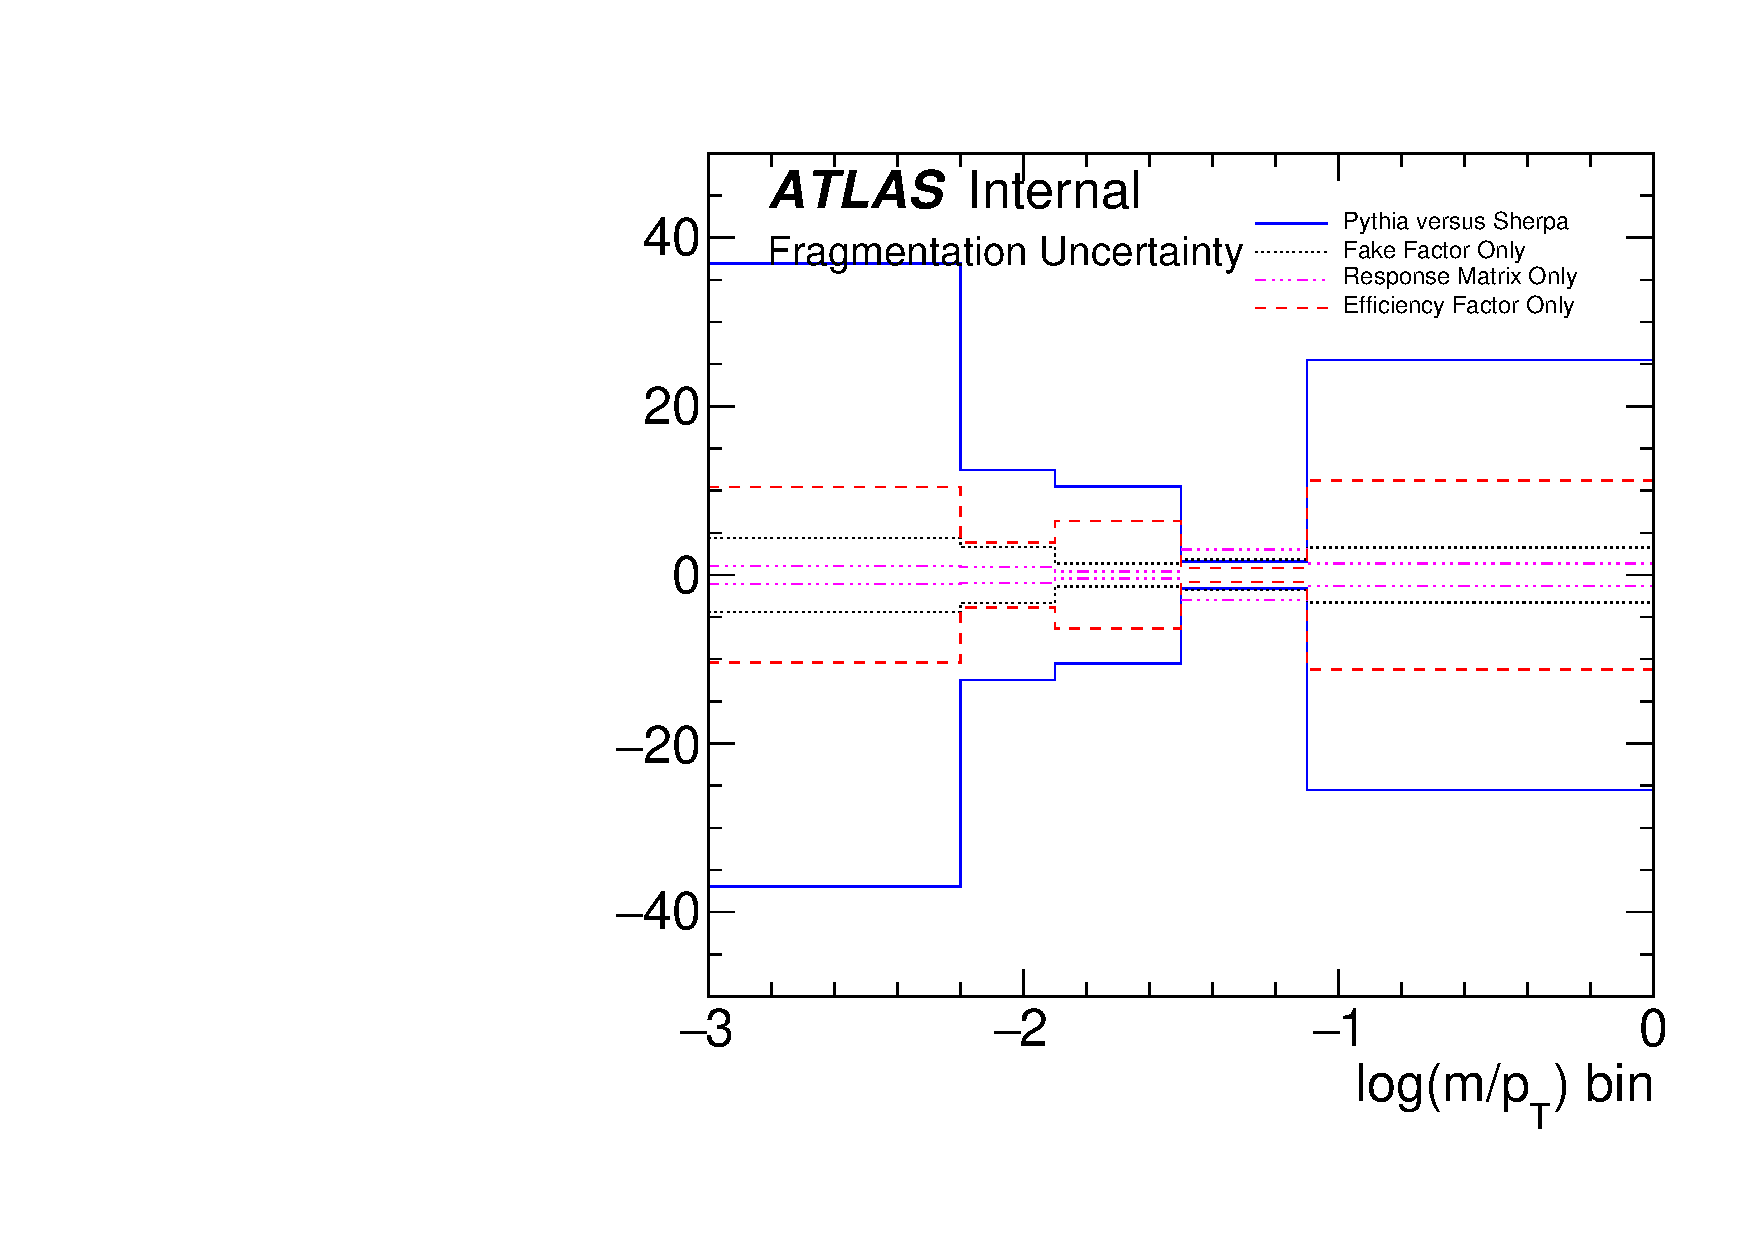
\includegraphics[width=0.45\linewidth]{figures/gbb/Unfolding/fracmasspt0_uncert_summary.pdf}
%\caption[]{A summary of the fragmentation modeling uncertainty for all four observables.  The blue solid line compares Pythia with Sherpa with significant double-counting with the non-closure uncertainty.  The fake- (efficiency-)factor line uses Pythia with the fake- (efficiency-)factor replaced by the one from Sherpa.  Finally, the response matrix only line uses the Pythia response matrix, but re-weighted so that the particle-level projection is the Sherpa particle-level distribution.  The fragmentation modeling uncertainty is the sum in quadrature of these last three components. } 
%\label{fig:syst_overview_deltaR2frag}
%\end{center}
%\end{figure}
%
%\begin{figure}[htpb!]
%\begin{center}
%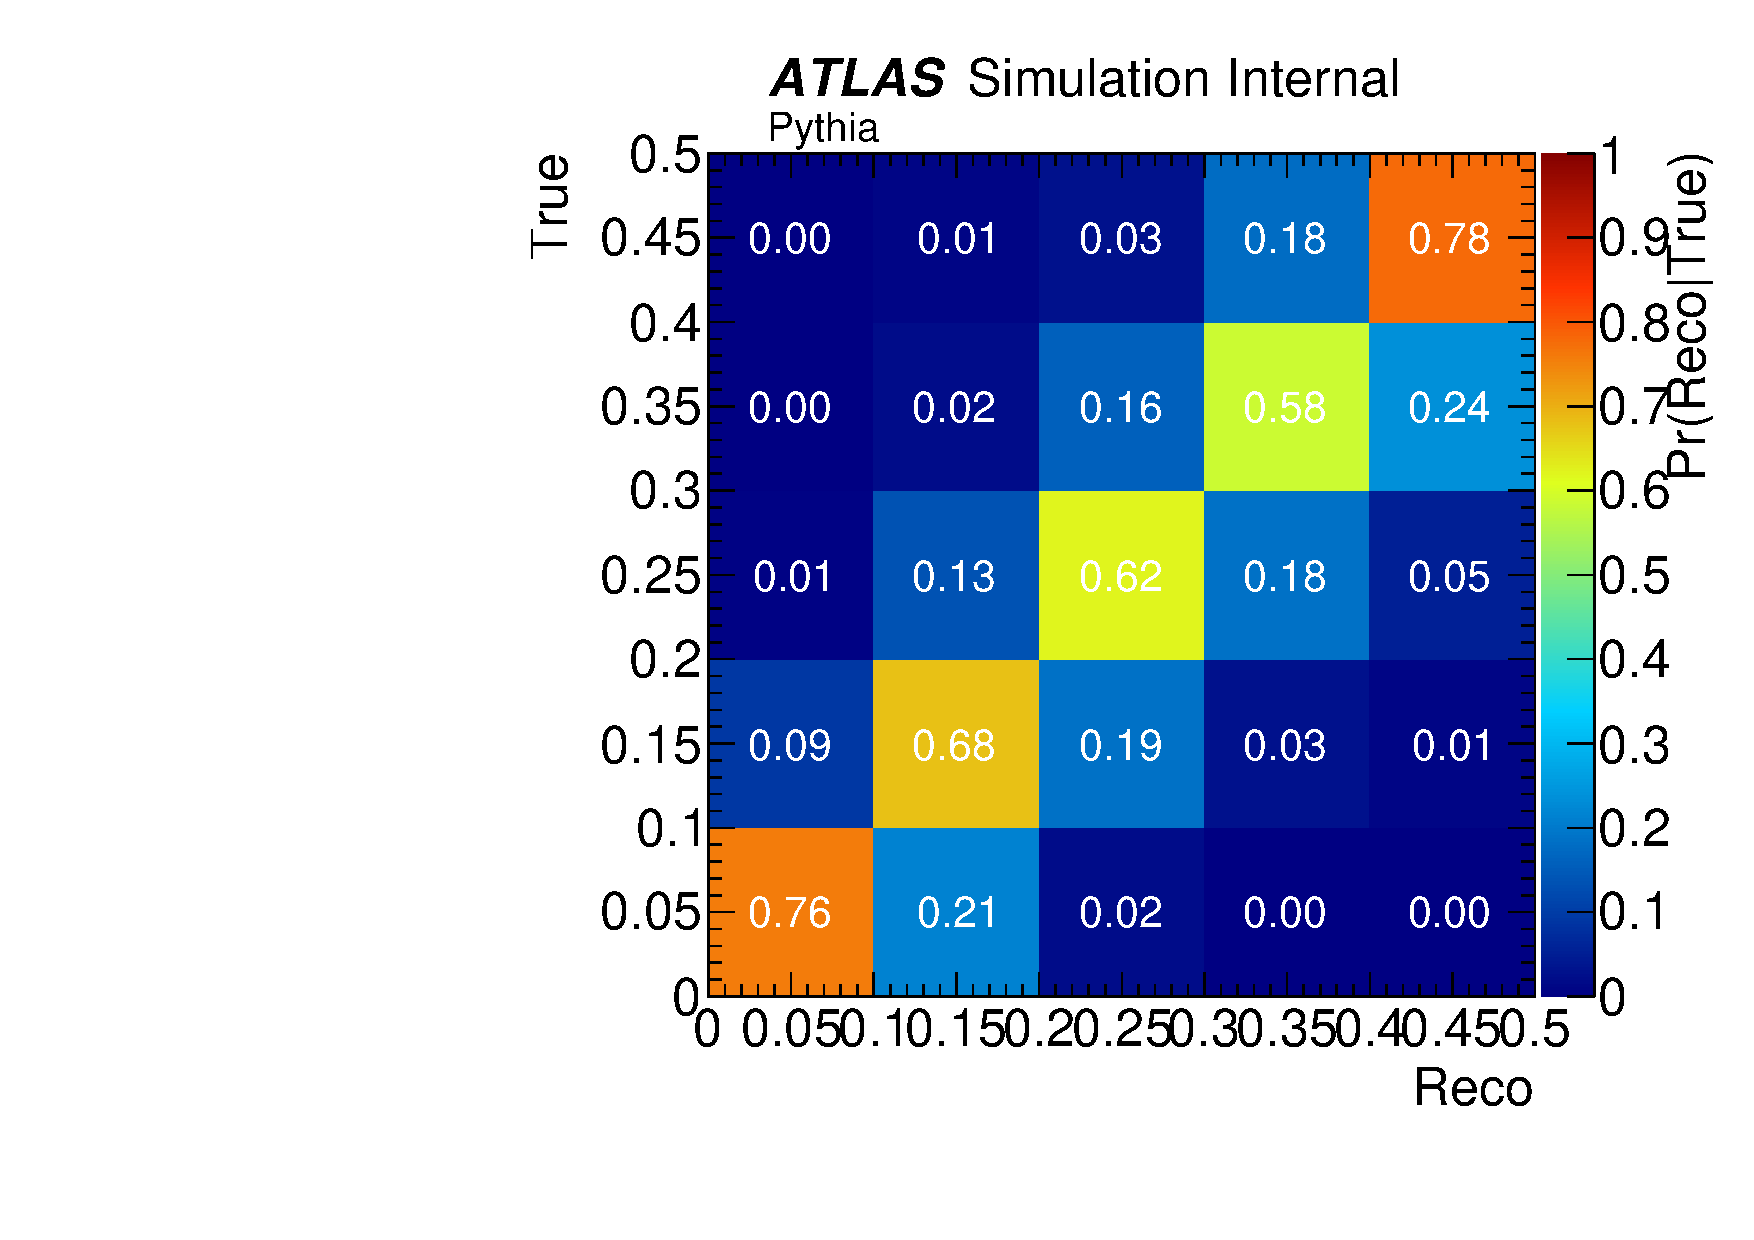
\includegraphics[width=0.3\linewidth]{figures/gbb/Unfolding/testPythiaZpT.pdf}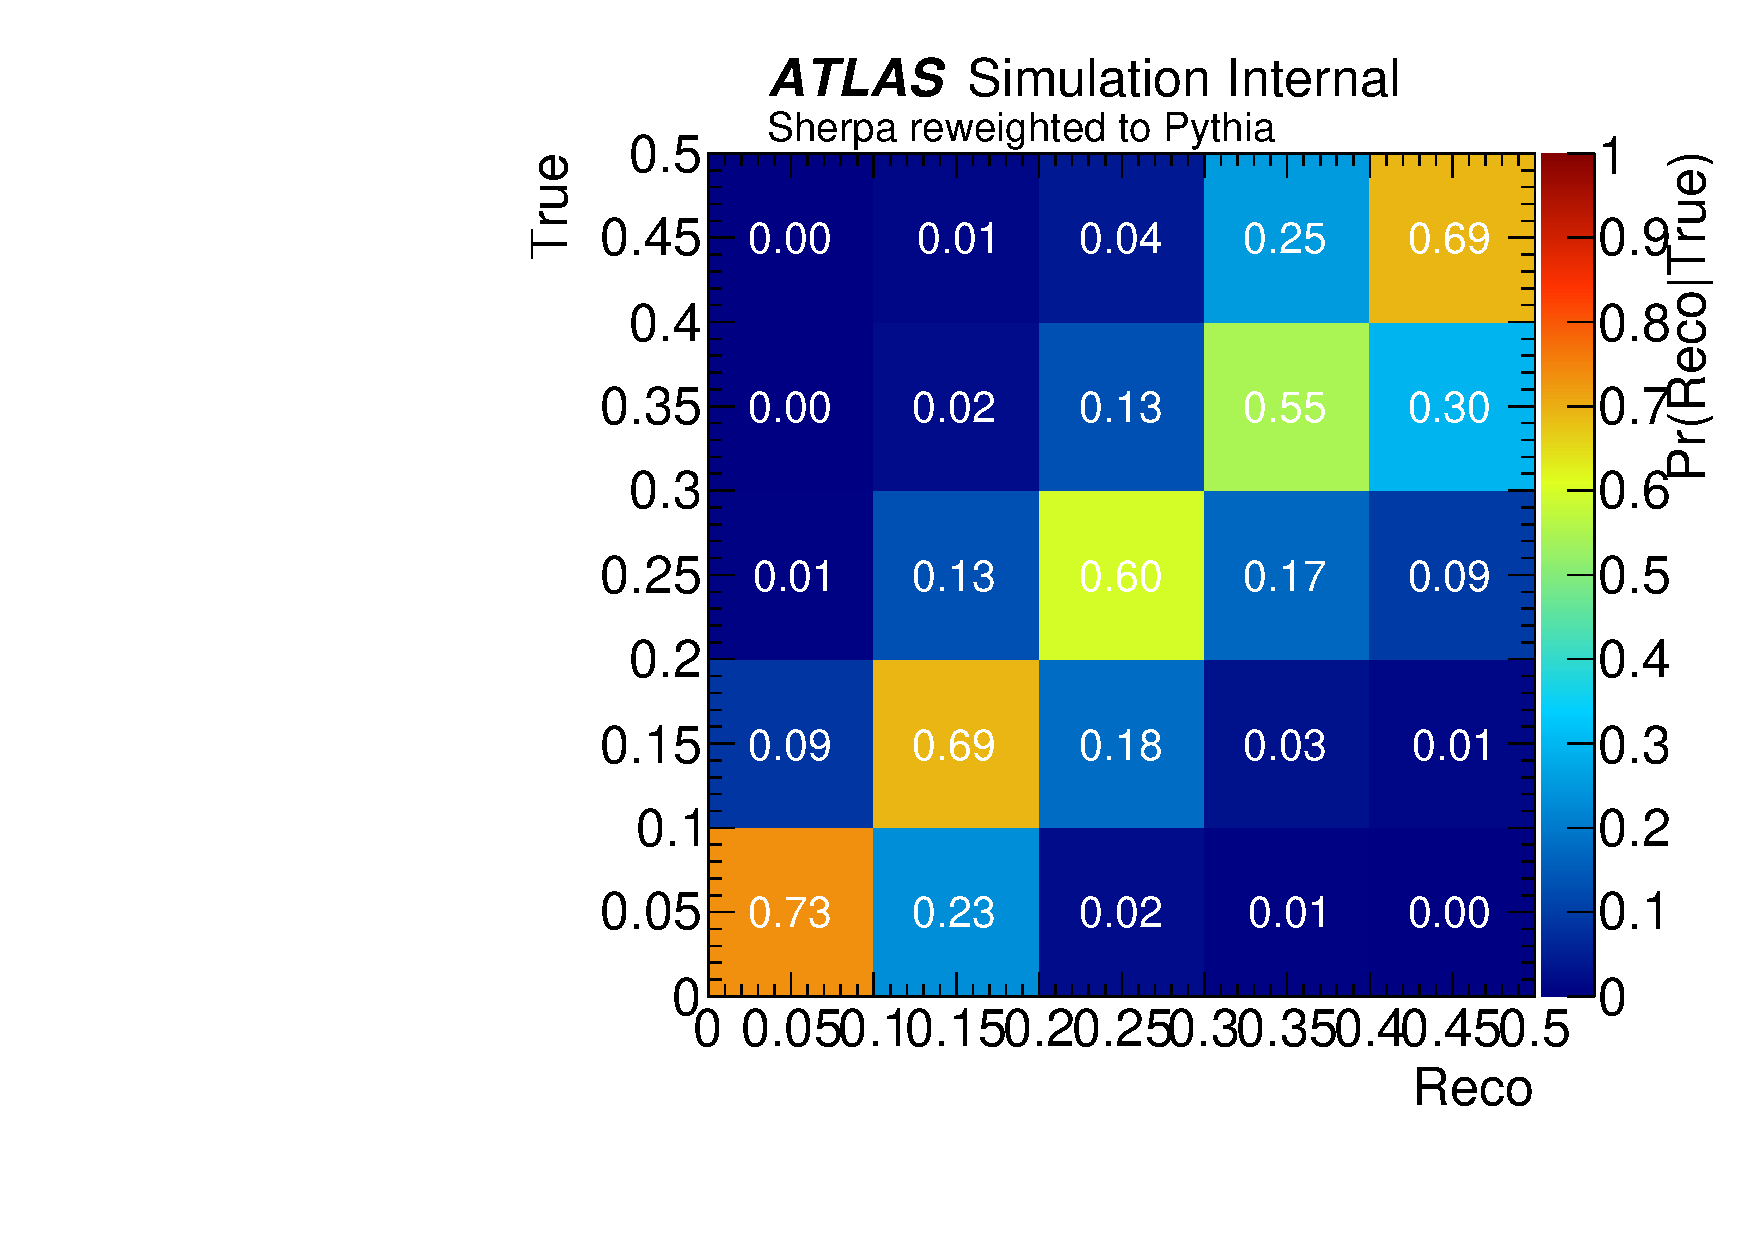
\includegraphics[width=0.3\linewidth]{figures/gbb/Unfolding/testSherpaZpT.pdf}
%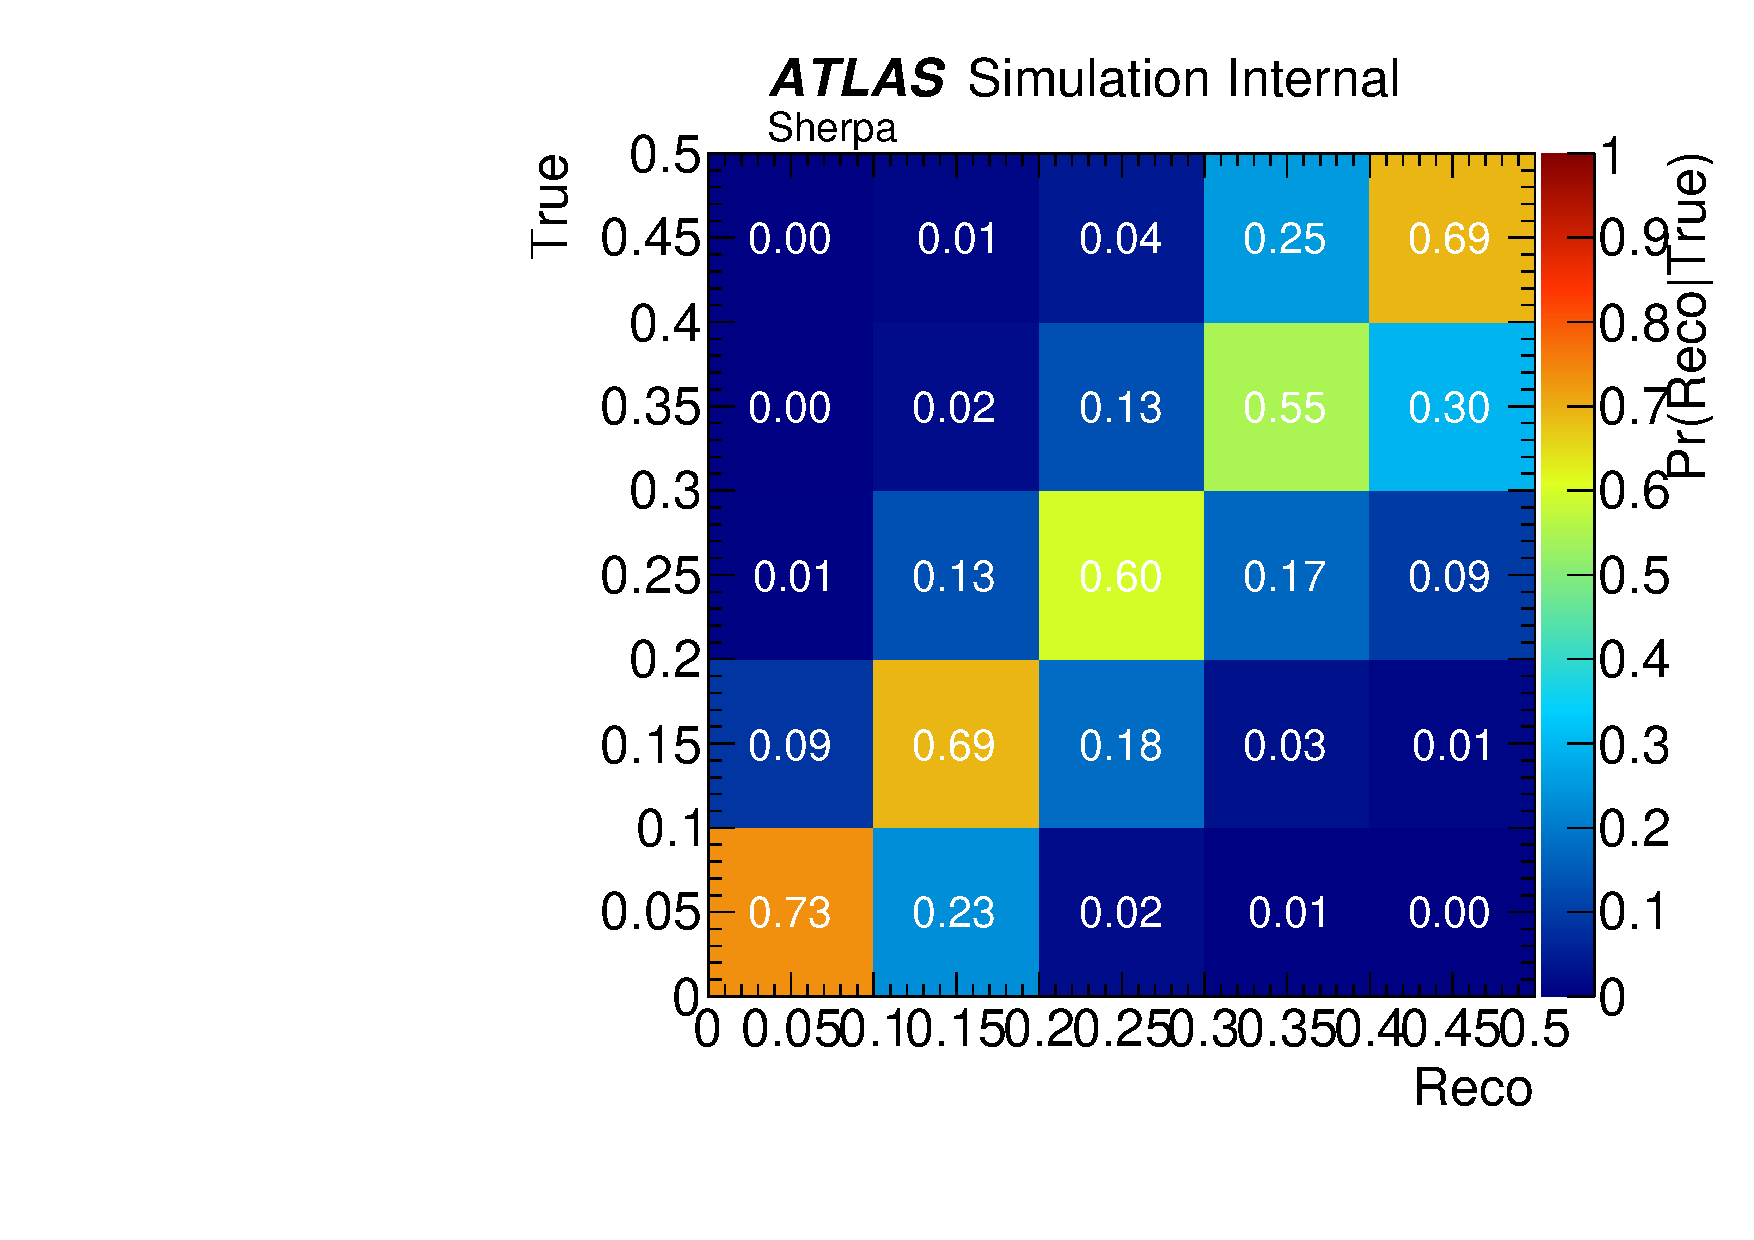
\includegraphics[width=0.3\linewidth]{figures/gbb/Unfolding/testSherpa_norwZpT.pdf}\\
%
%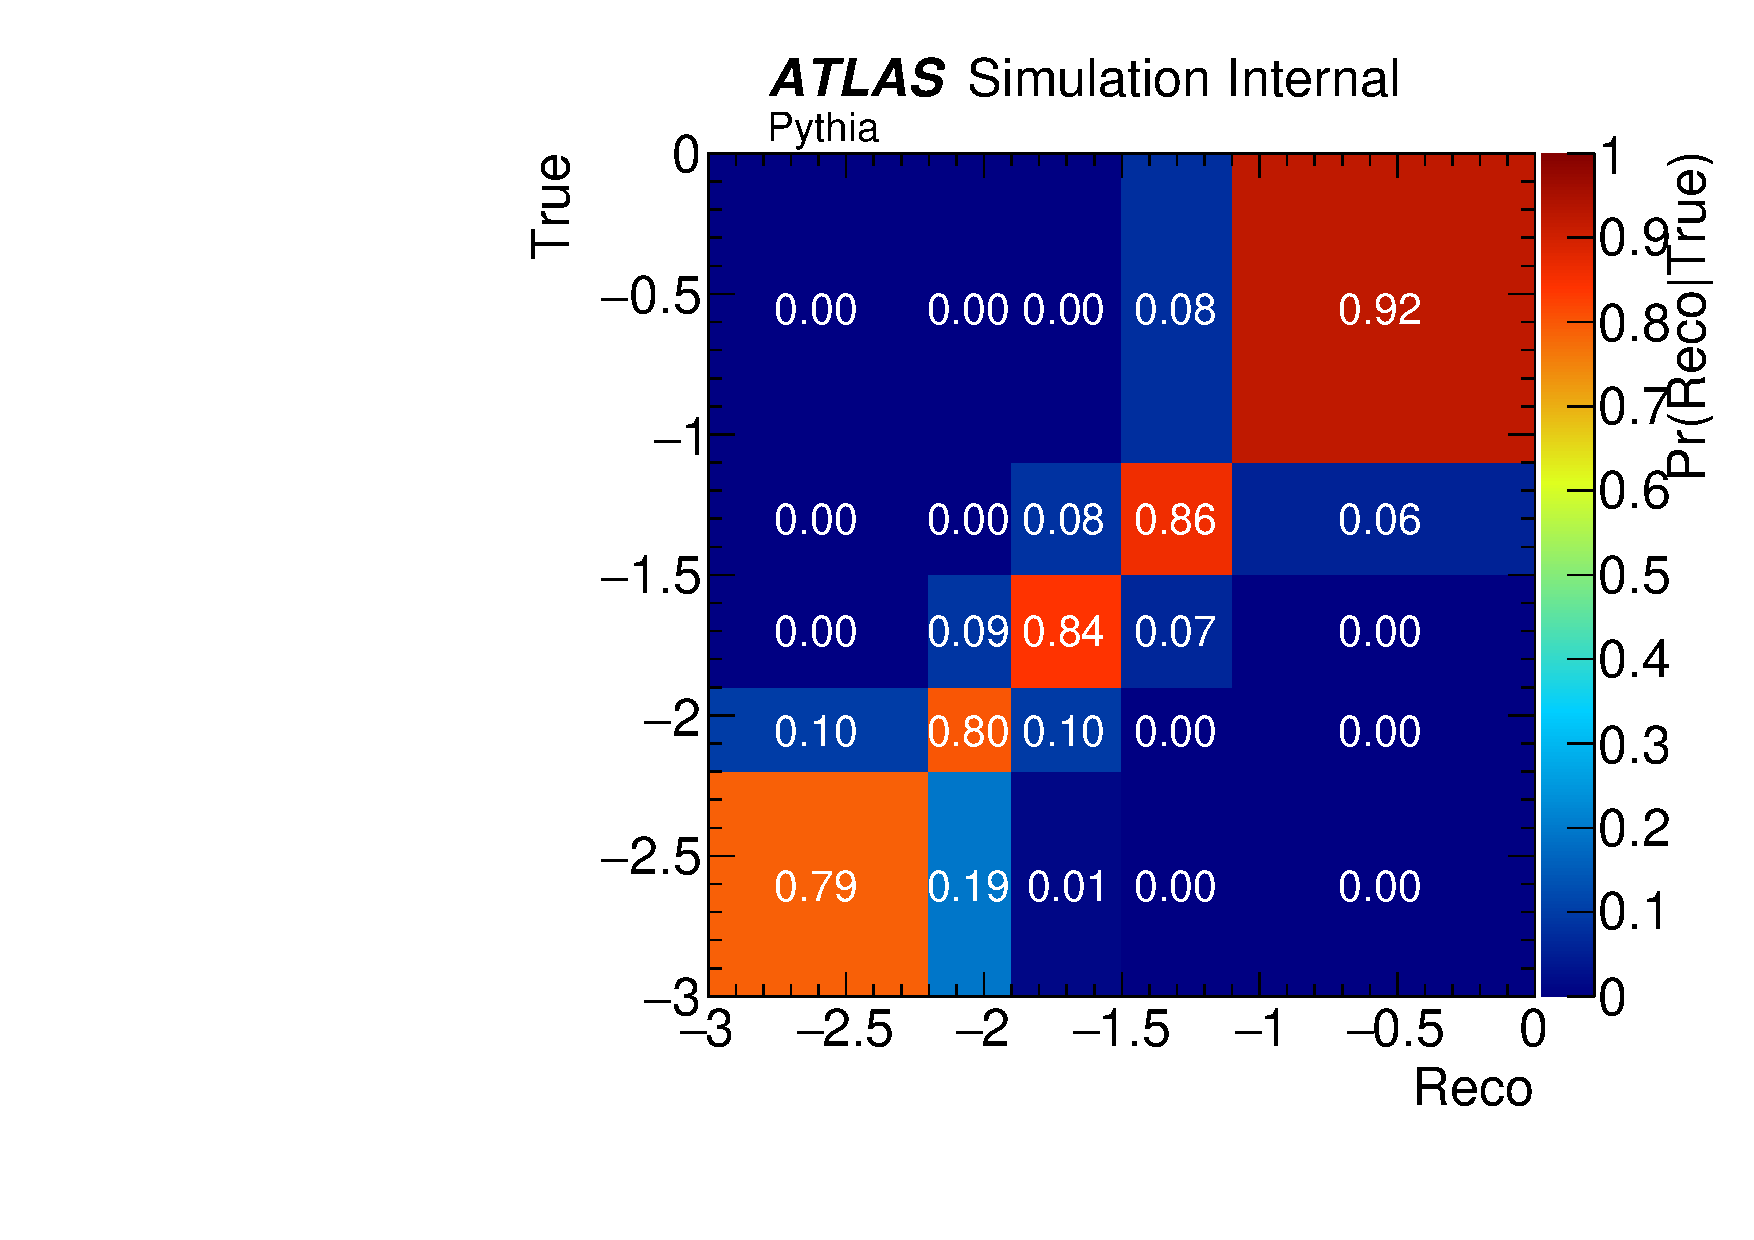
\includegraphics[width=0.3\linewidth]{figures/gbb/Unfolding/testPythiafracmasspt.pdf}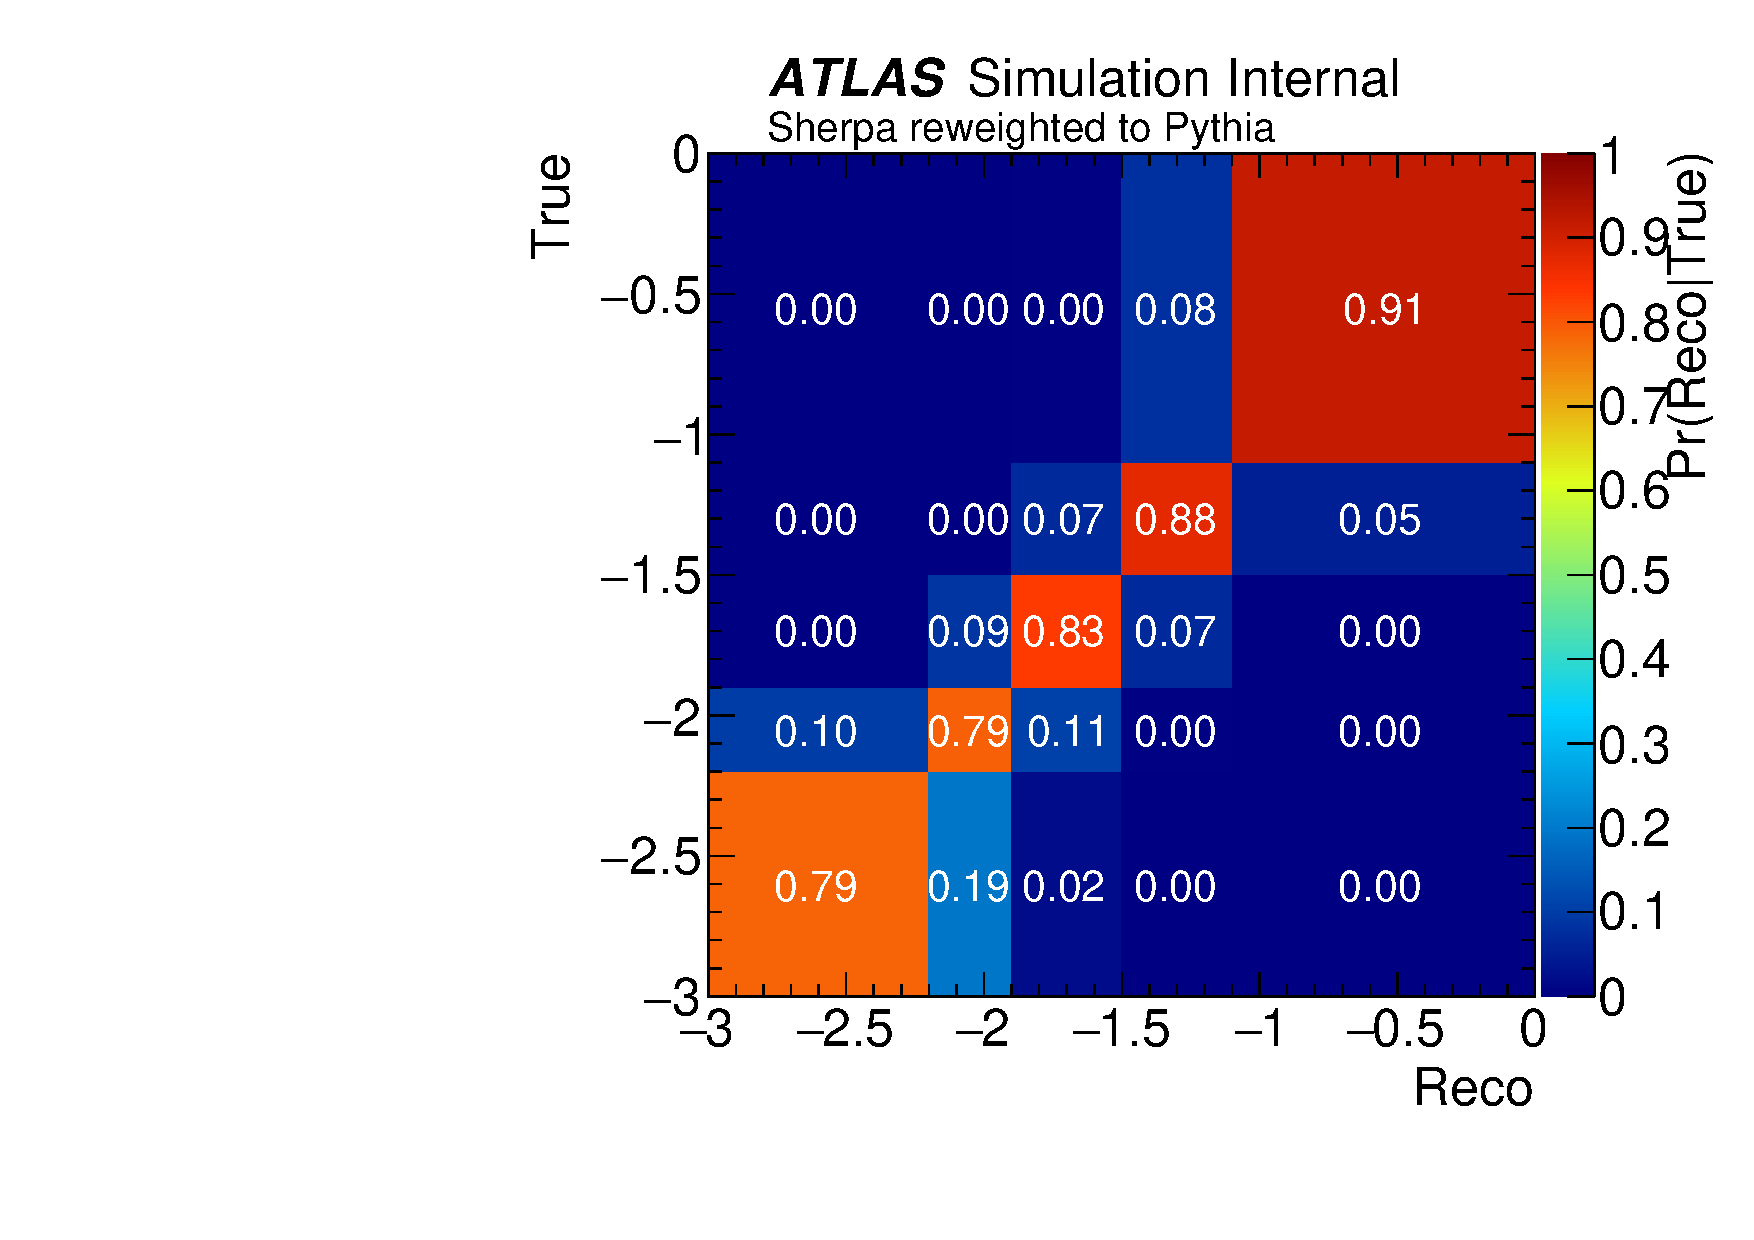
\includegraphics[width=0.3\linewidth]{figures/gbb/Unfolding/testSherpafracmasspt.pdf}
%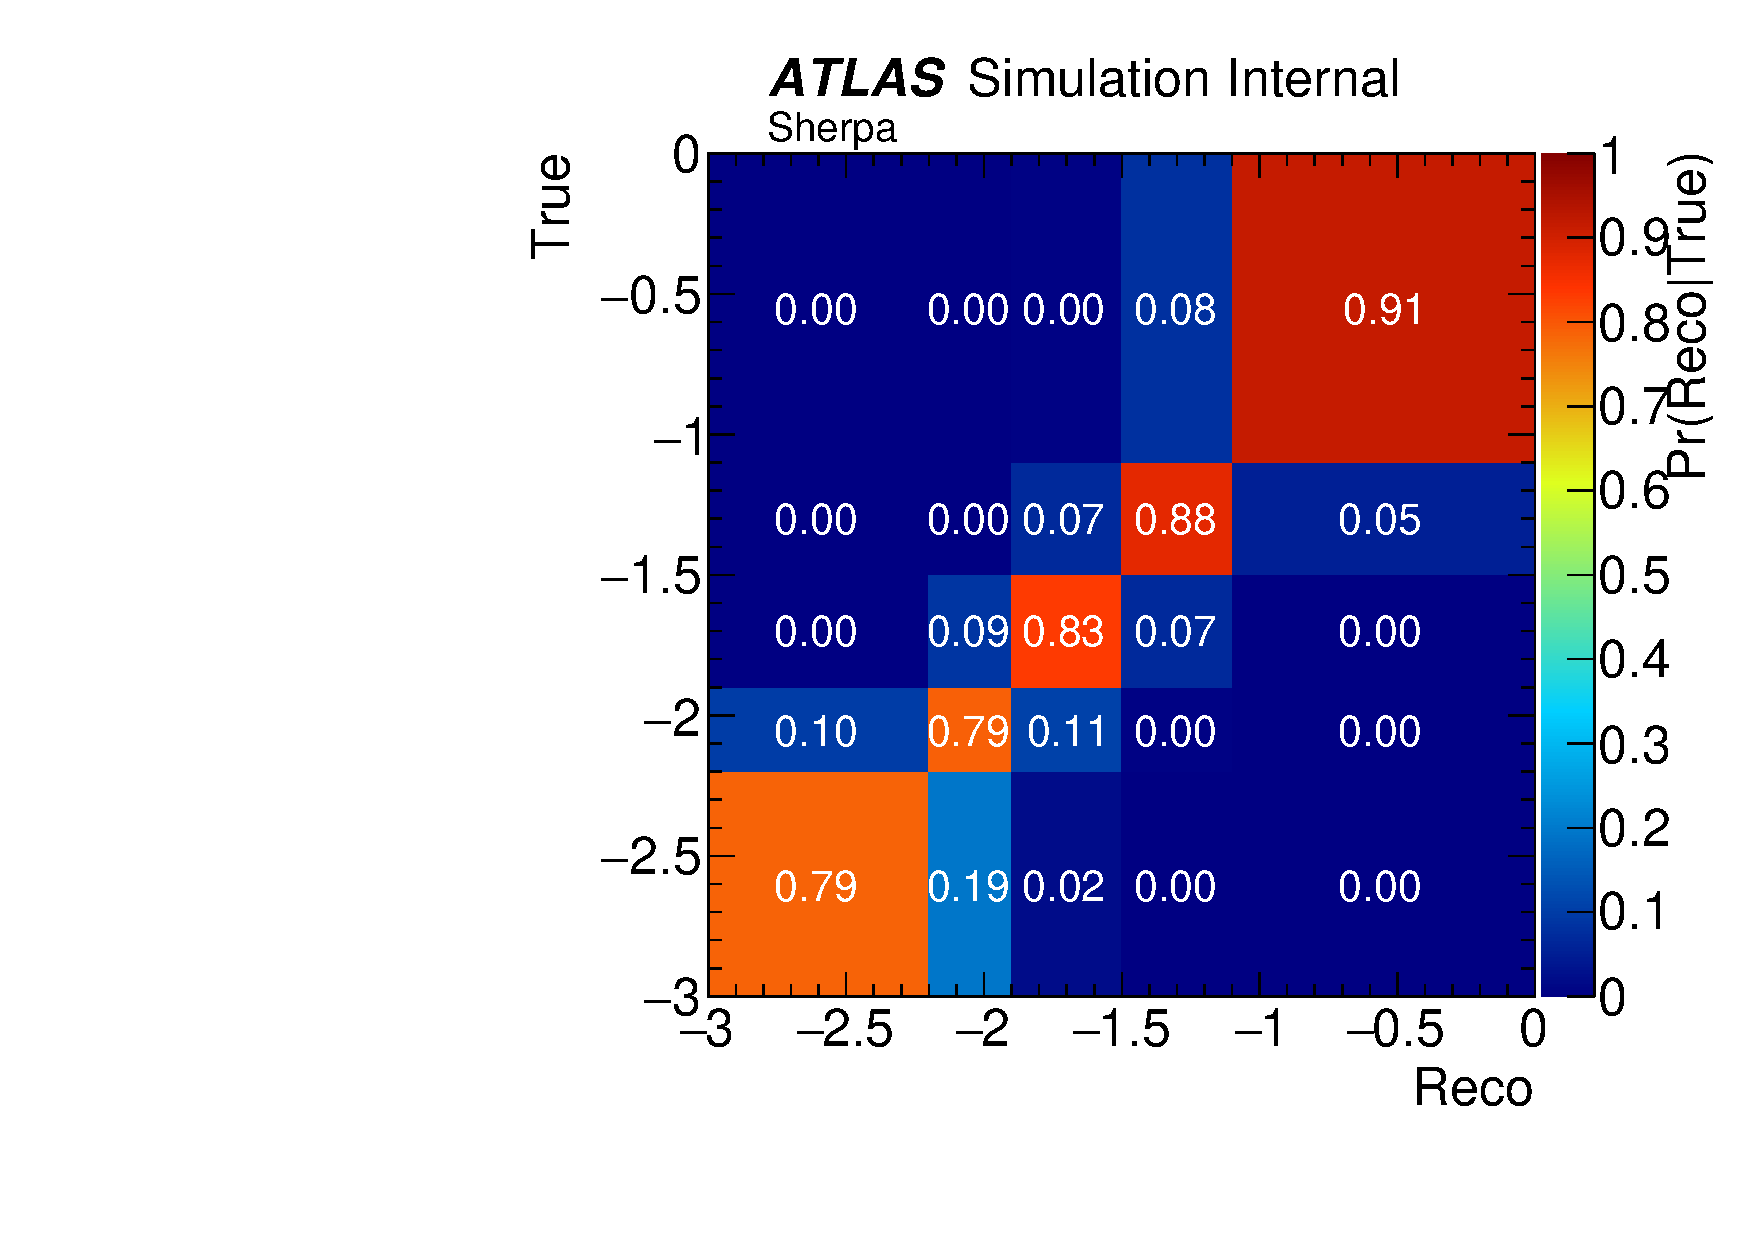
\includegraphics[width=0.3\linewidth]{figures/gbb/Unfolding/testSherpa_norwfracmasspt.pdf}\\
%
%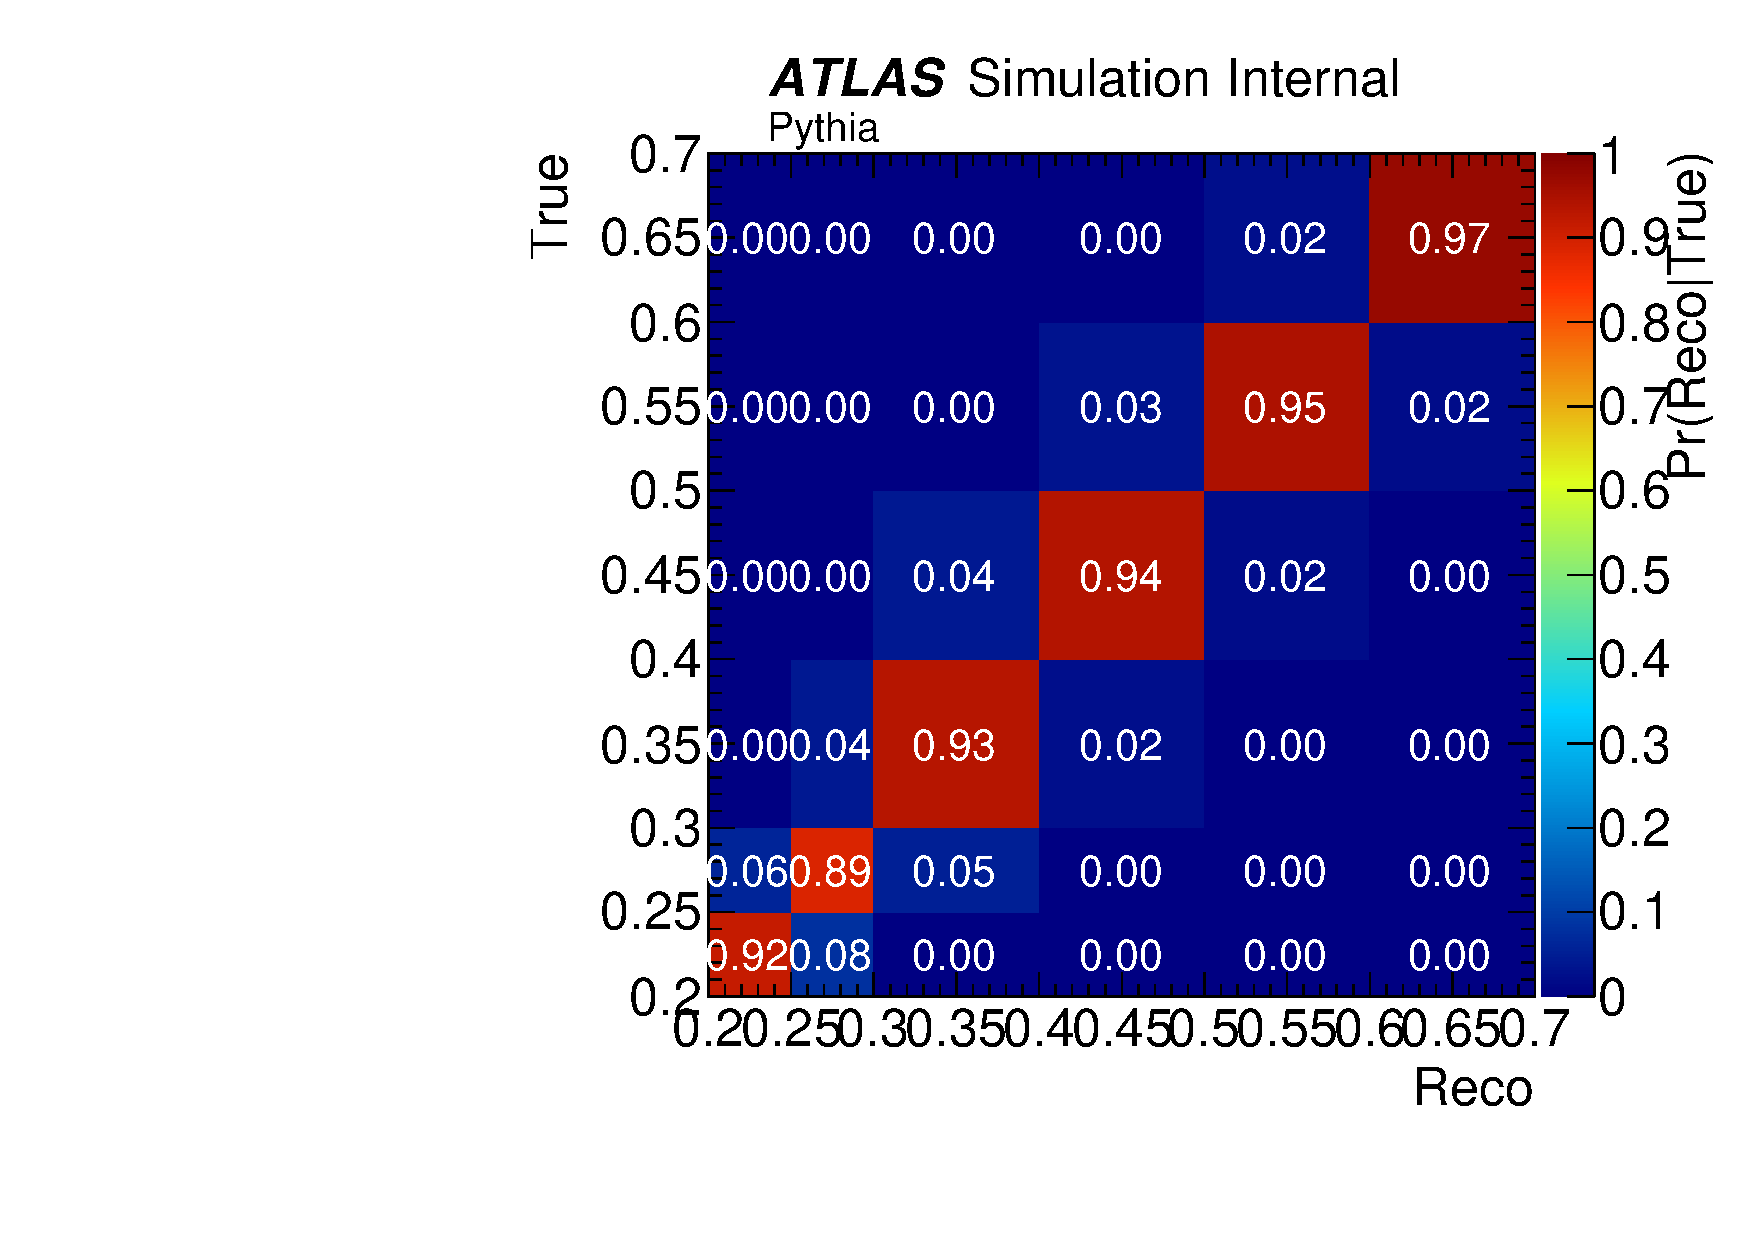
\includegraphics[width=0.3\linewidth]{figures/gbb/Unfolding/testPythiadR.pdf}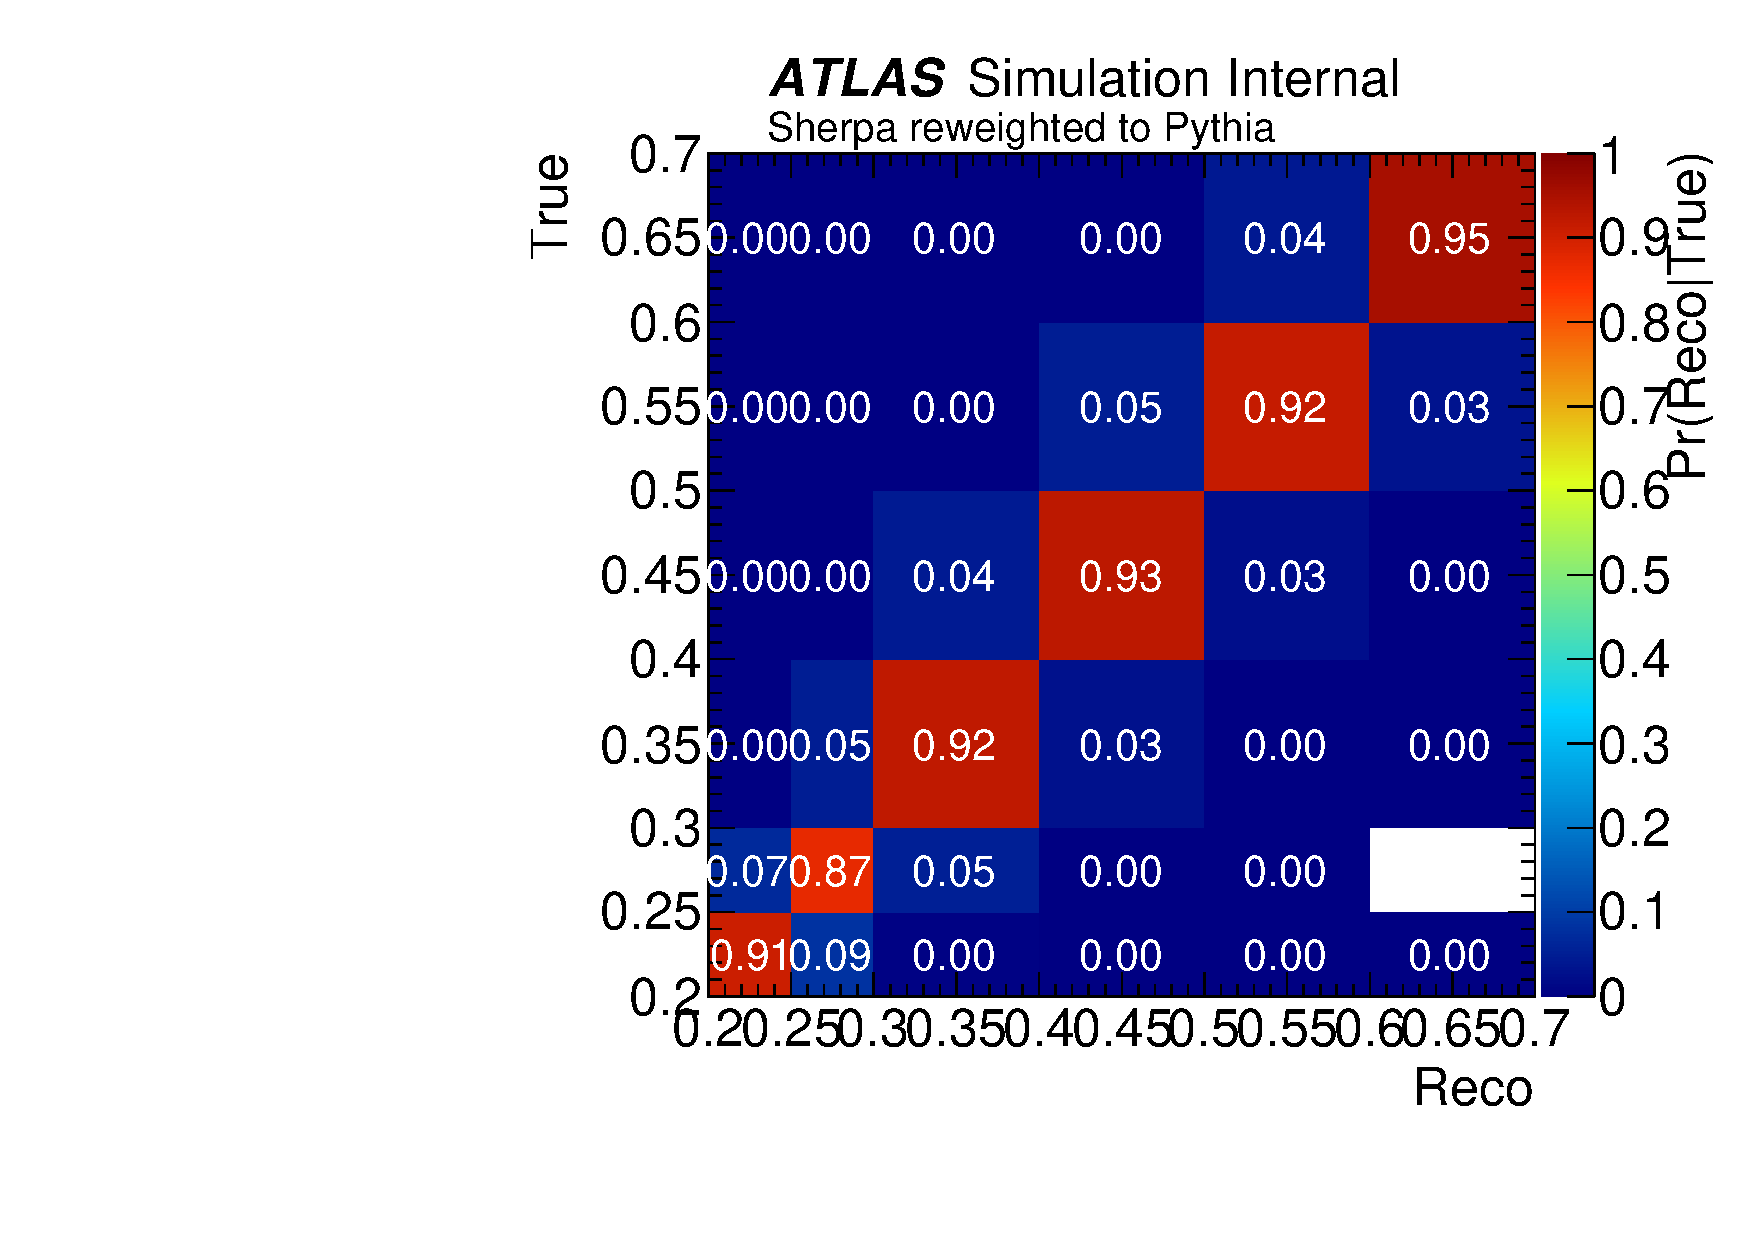
\includegraphics[width=0.3\linewidth]{figures/gbb/Unfolding/testSherpadR.pdf}
%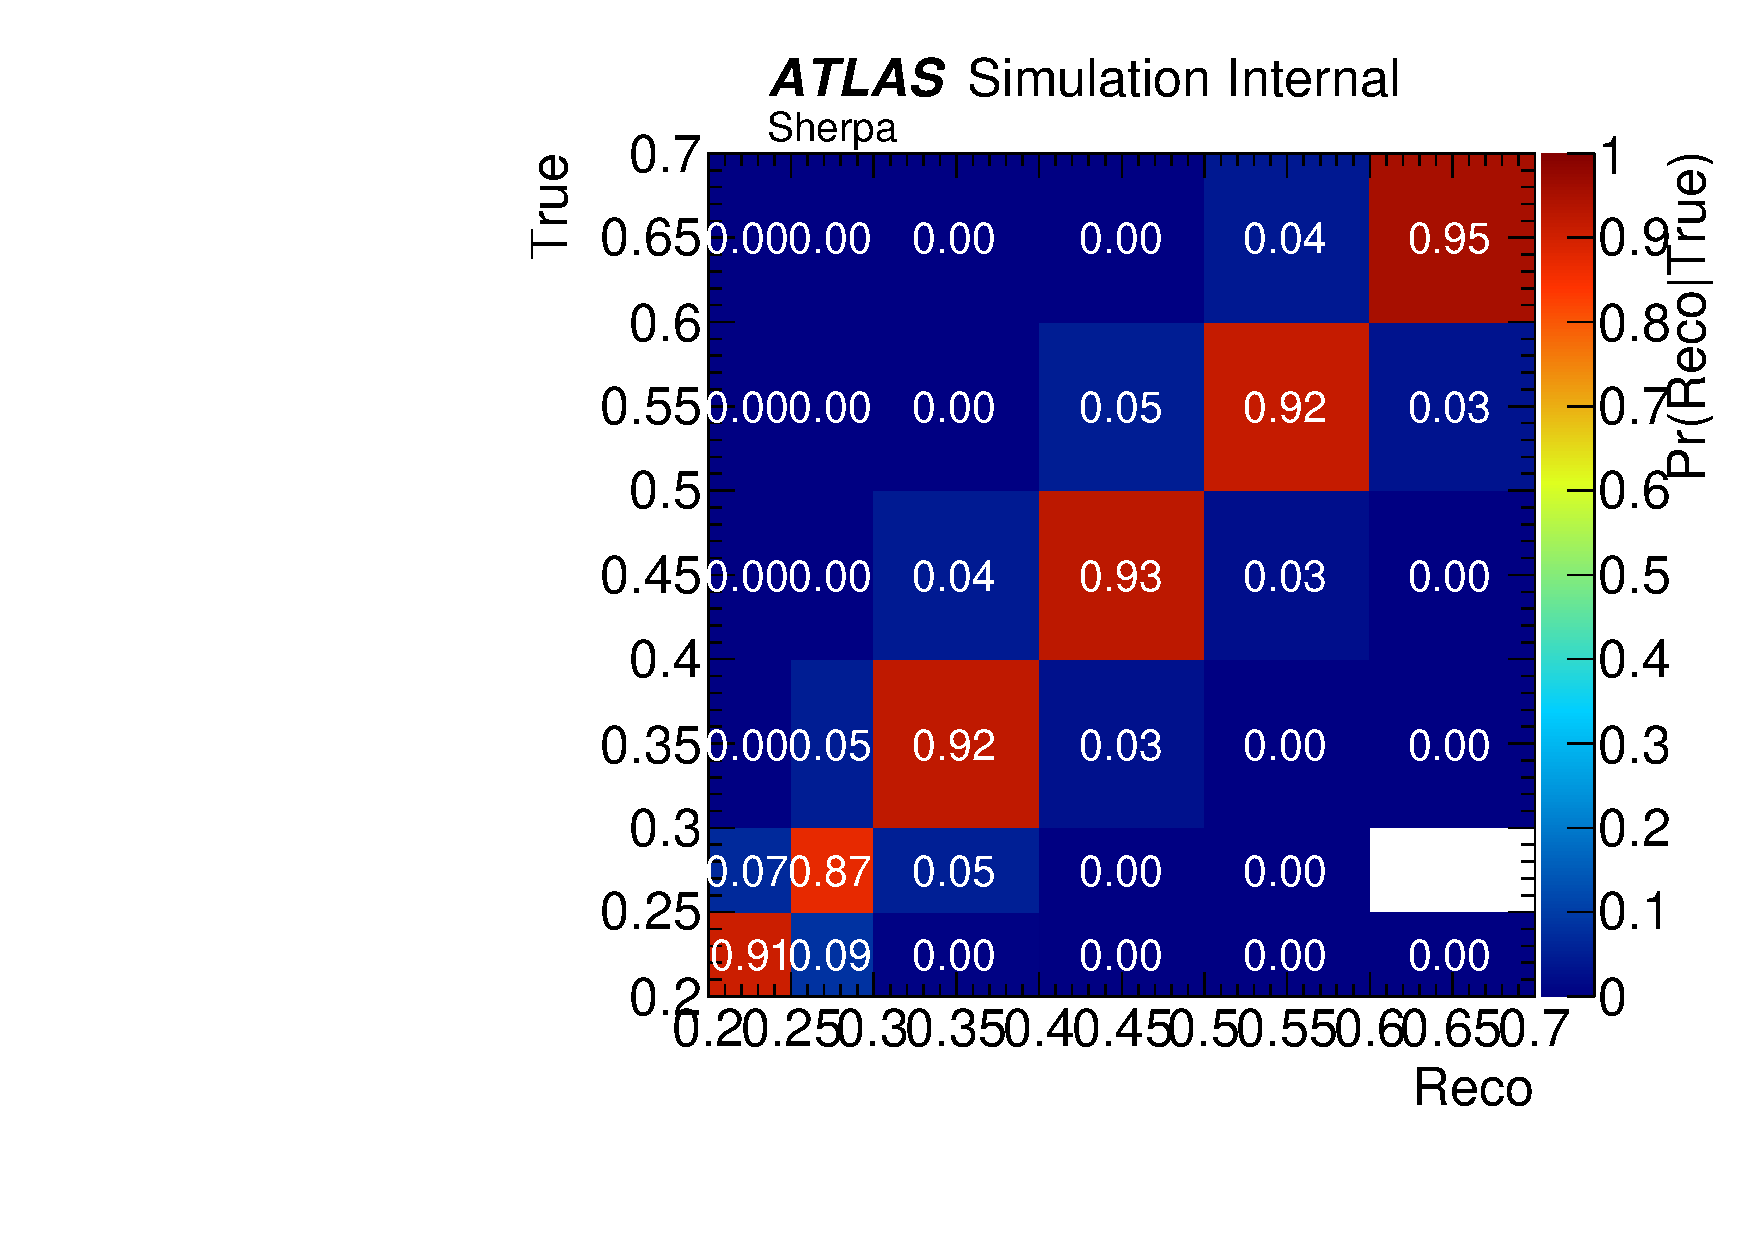
\includegraphics[width=0.3\linewidth]{figures/gbb/Unfolding/testSherpa_norwdR.pdf}\\
%
%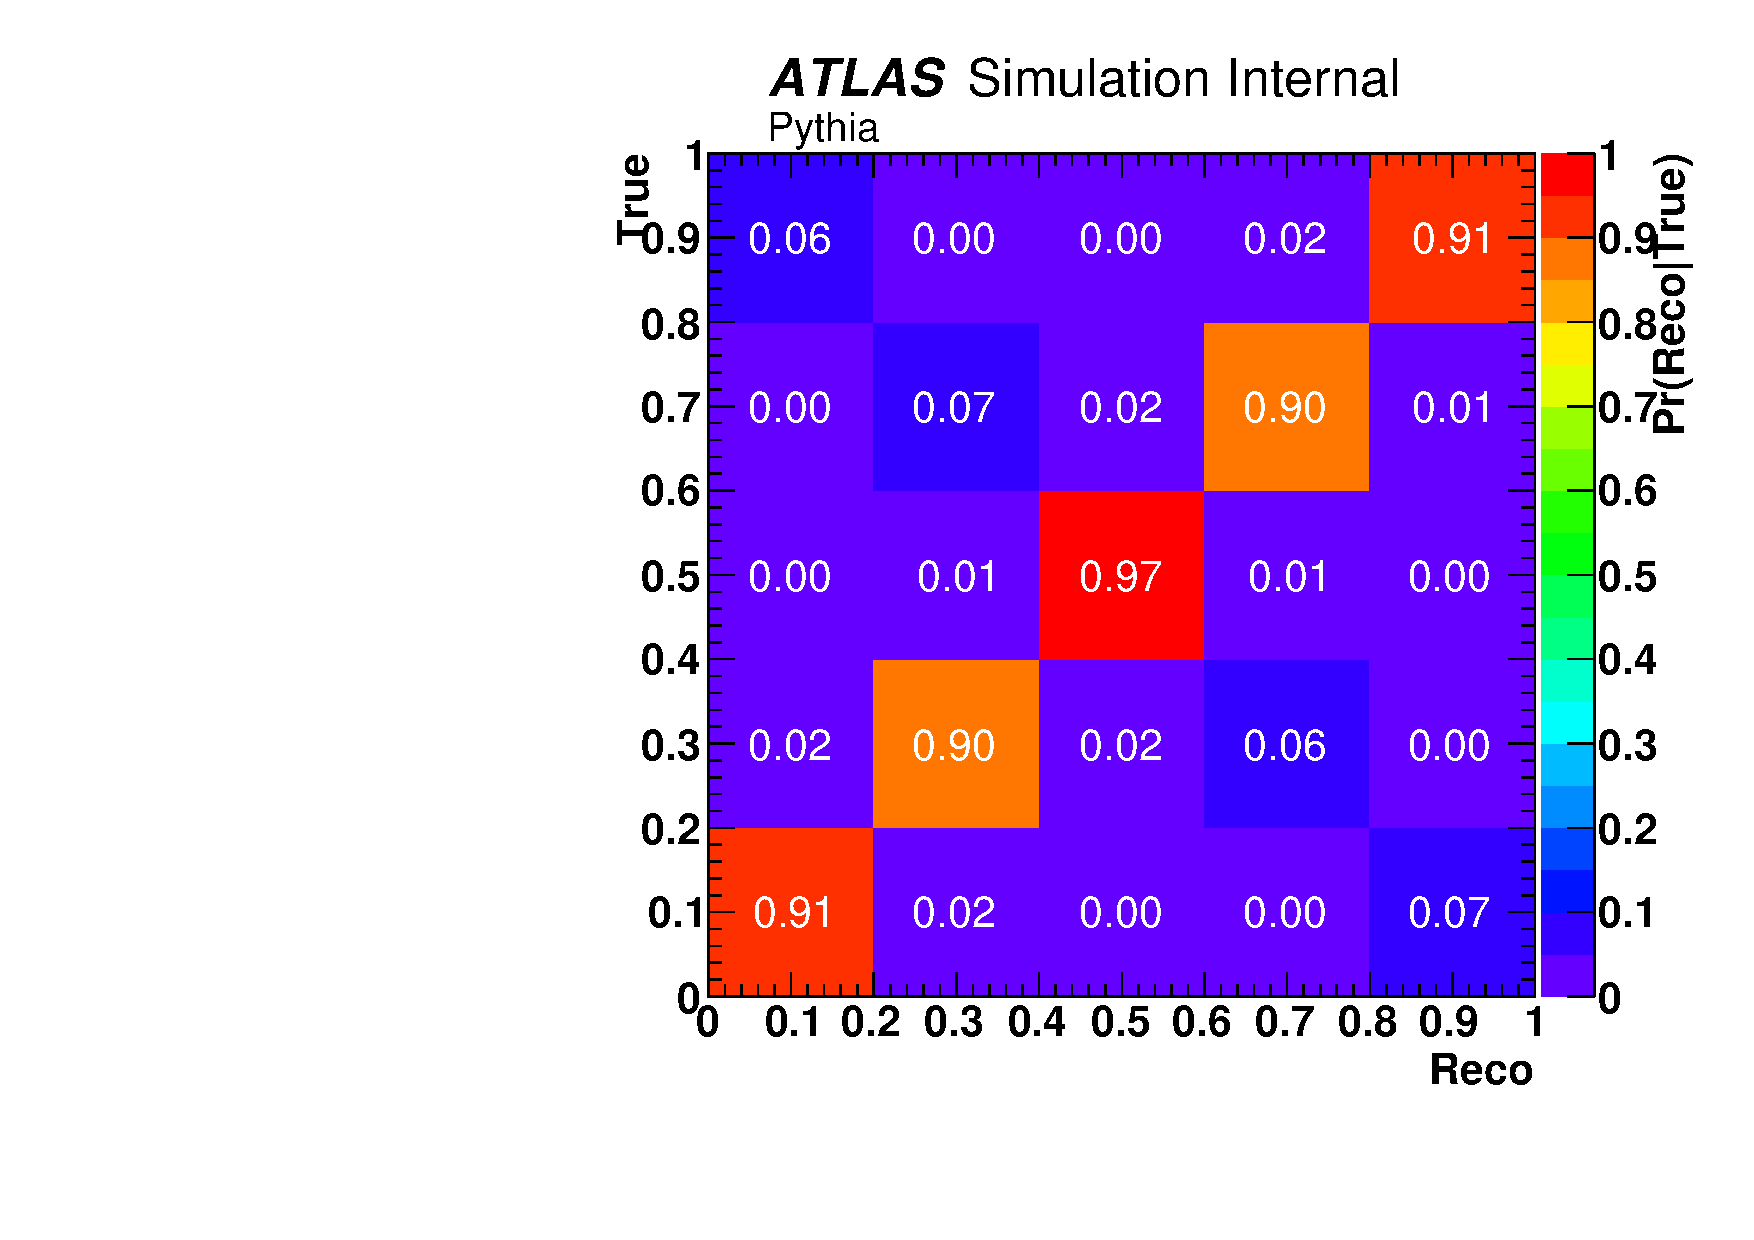
\includegraphics[width=0.3\linewidth]{figures/gbb/Unfolding/testPythiadphi.pdf}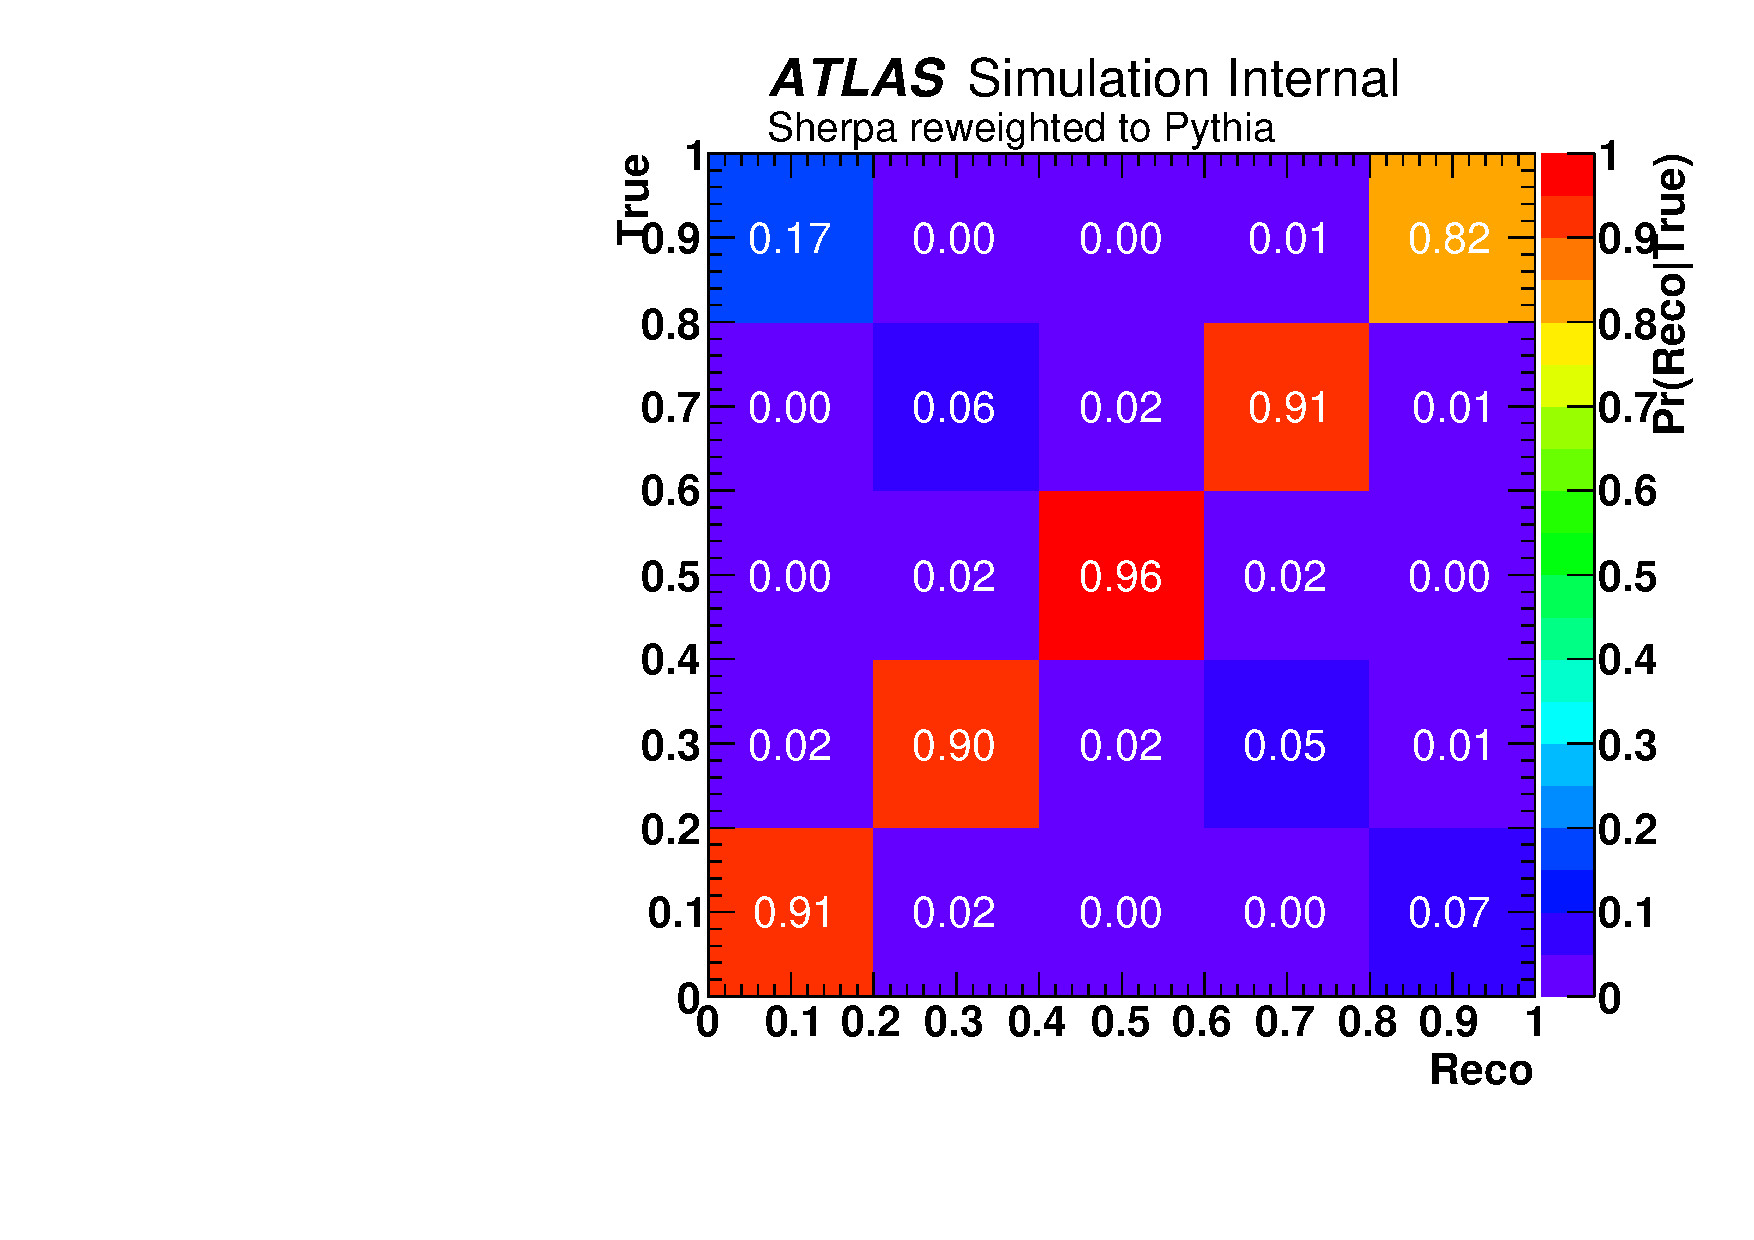
\includegraphics[width=0.3\linewidth]{figures/gbb/Unfolding/testSherpadphi.pdf}
%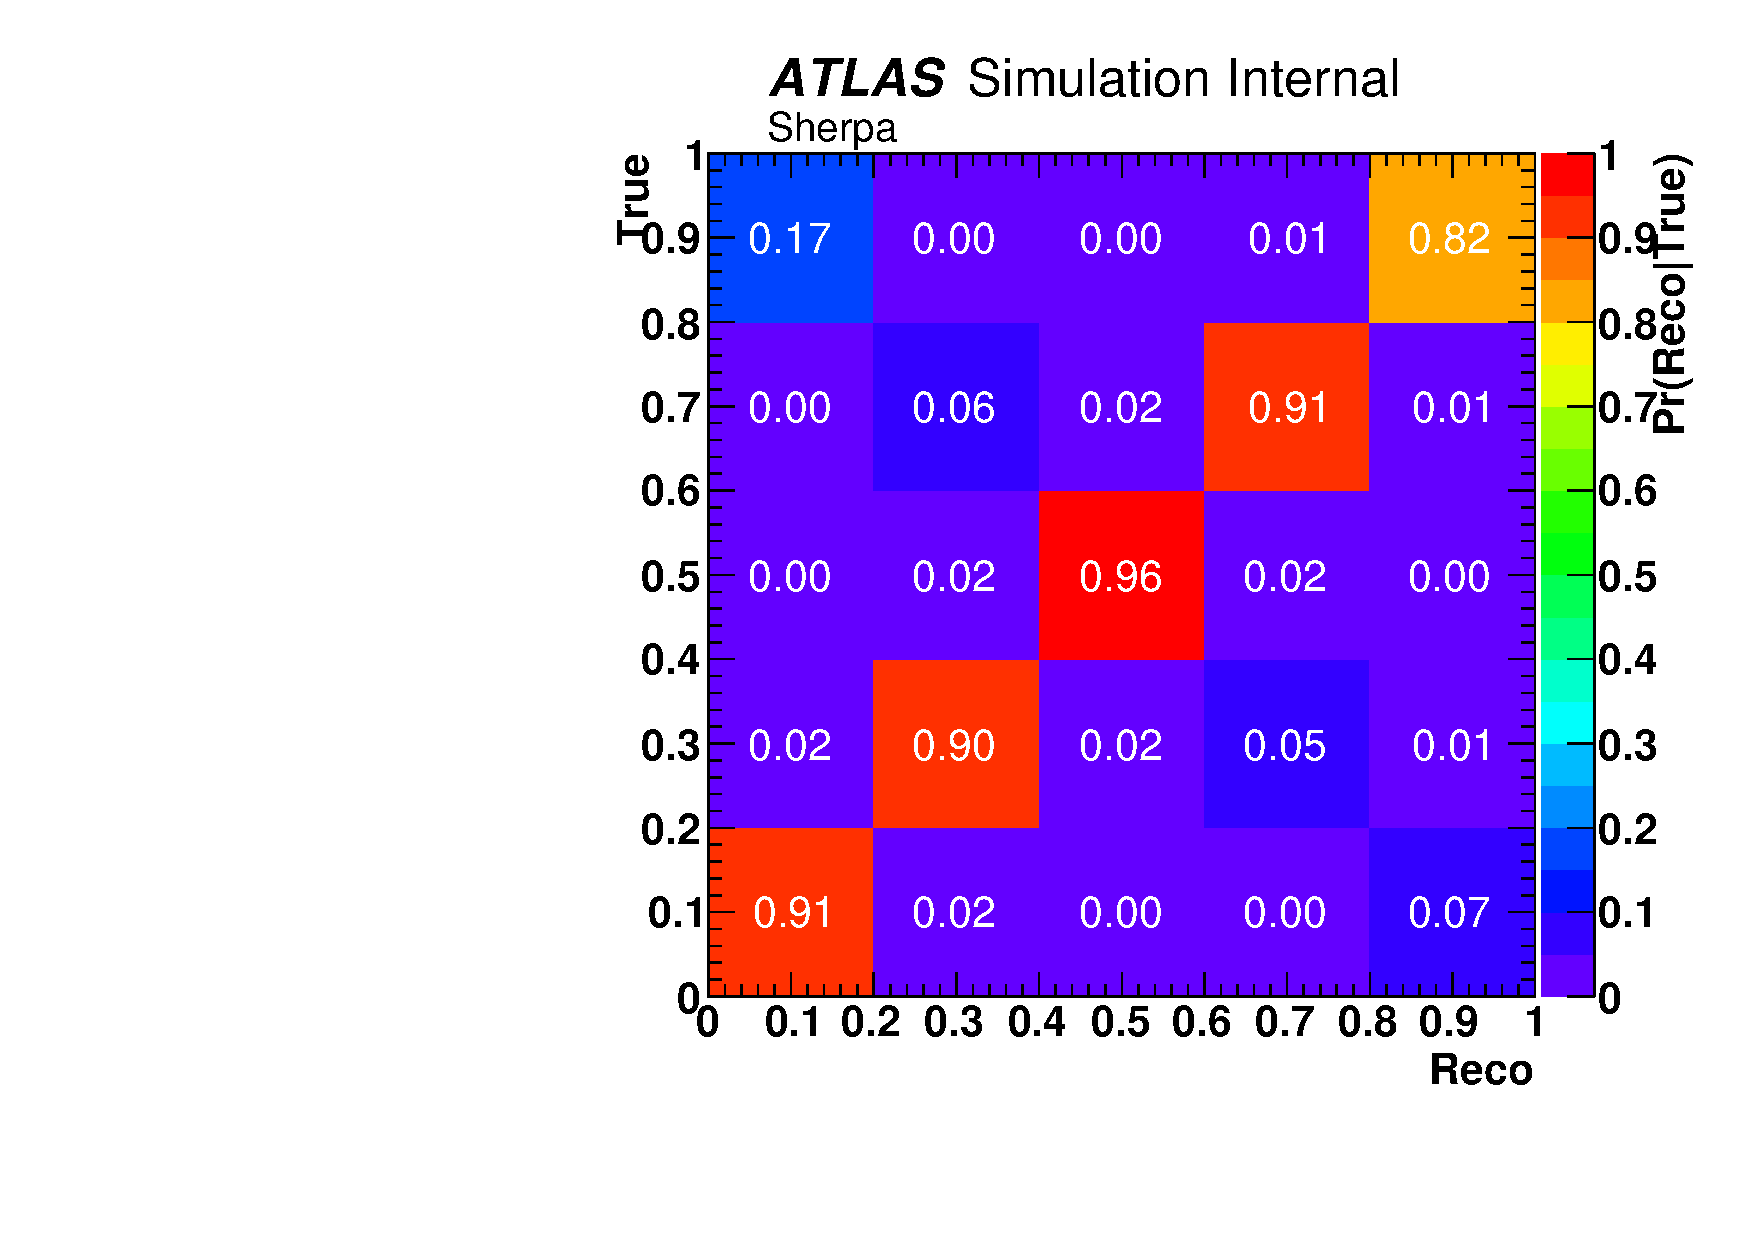
\includegraphics[width=0.3\linewidth]{figures/gbb/Unfolding/testSherpa_norwdphi.pdf}
%
%\caption[]{A detector-level comparison between Pythia, Sherpa, and data.  The MC is normalized to the data.} 
%\label{fig:frag2}
%\end{center}
%\end{figure}

\subsection{Unfolding Non-closure}
\label{sec:gbb-systs:unfolding}

The standard method~\cite{Armbruster:1694351} for evaluating the systematic uncertainty from the procedure is to re-weight the MC to the data and take the difference between the unfolded re-weighted reconstructed MC to the truth MC of the same generator.

%The re-weighted truth is a \textit{reasonable} prior with which we can estimate the bias from the choice of prior in the unfolding method.   Define the following histograms ($x_i$ will interchangeably mean the histogram $x$ and also the content in the $i^{th}$ bin of $x$):
%
%\begin{description}
%\item[$d_i$]: The measured spectrum. 
%\item[$R_{ij}$]: The response matrix such that $R_{ij}$ contains the number of events in the simulation that fall in the reconstructed bin $i$ and the truth bin $j$.
%\item[$t_i$]: $t_i = \sum_j R_{ji}$, i.e. the truth spectrum for events that pass both truth and reconstructed selections.
%\item[$r_i$]: $r_i = \sum_j R_{ij}$, i.e. the reconstructed spectrum for events that pass both truth and reconstructed selections
%\item[$\tilde{R}_{ij}$]: The normalized version of $R_{ij}$ such that $r_i = \sum_j \tilde{R}_{ij} t_j$.  Explicitly, $\tilde{R}_{ij} = R_{ij}/\sum_{i'} R_{i'j}$.  The entries of $\tilde{R}_{ij}$ are the conditional probability for a truth event in bin $j$ to be reconstructed in bin $i$.
%\end{description}
%
%\noindent The re-weighting procedure can only be applied to simulation events which pass both the truth and reconstructed event selections and so the first step is to take the data and apply a correction $\epsilon_i$ bin-by-bin given by 
%
%\begin{align}
%\epsilon_i = \frac{\text{Pass both reconstructed and truth selections}}{\text{Pass the reconstructed selection}},
%\end{align}
%
%\noindent where $i$ is the bin number.   Define $\tilde{d}_i = \epsilon_i d_i$ to be the corrected data histogram.  We want now a prior $\tilde{t}_i$ such that $\tilde{R}_{ij} \tilde{t}_j$ is very close to $\tilde{d}_i$.  Since $\tilde{R}_{ij}$ is not too far from a diagonal matrix, one way of generating $\tilde{t}_i$ is to use weights built from the reconstructed simulation: $w_i = \tilde{d}_i/r_i$.  Define $\tilde{t}_i=w_it_i$.  Fig. X shows that the weights $w_i$ are effective at improving the data/MC agreement of $\tilde{r}_i=\sum_j\tilde{R}_{ij}\tilde{t}_j$ with respect to $r_i$.  The non-closure uncertainty is then given by
%
%\begin{align}
%\sigma_i=\text{Unfold[nominal response matrix]}\left(\tilde{R}_{ij} \tilde{t}_j\right)-\tilde{t}_i
%\end{align}

%\textbf{In other words}, we have a function $f(d,p,R)$ which takes as inputs three histograms (data $d$, prior $p$, and the response matrix $R$) and outputs another histogram (the unfolding function).  By construction, $p=f(Rp,p,R)$ (not being careful about the normalization of $p$ and $R$, as above).  We pick $t$ such that $Rt\sim d$.  Then, the non-closure uncertainty is the difference between $f(Rt,p,R)$ and $t$.  The use of the word 'prior' is slightly misleading, since $p$ is still the prior used in the unfolding.

%Figure~\ref{fig:nonclosure1} shows the re-weighting factors and Fig.~\ref{fig:nonclosure2} shows that they work well, as expected since the response matrices are so diagonal.  The actual non-closure uncertainty is quite small and much smaller than the raw data/MC difference (Fig.~\ref{fig:nonclosure3}).
%
%\begin{figure}[htpb!]
%\begin{center}
%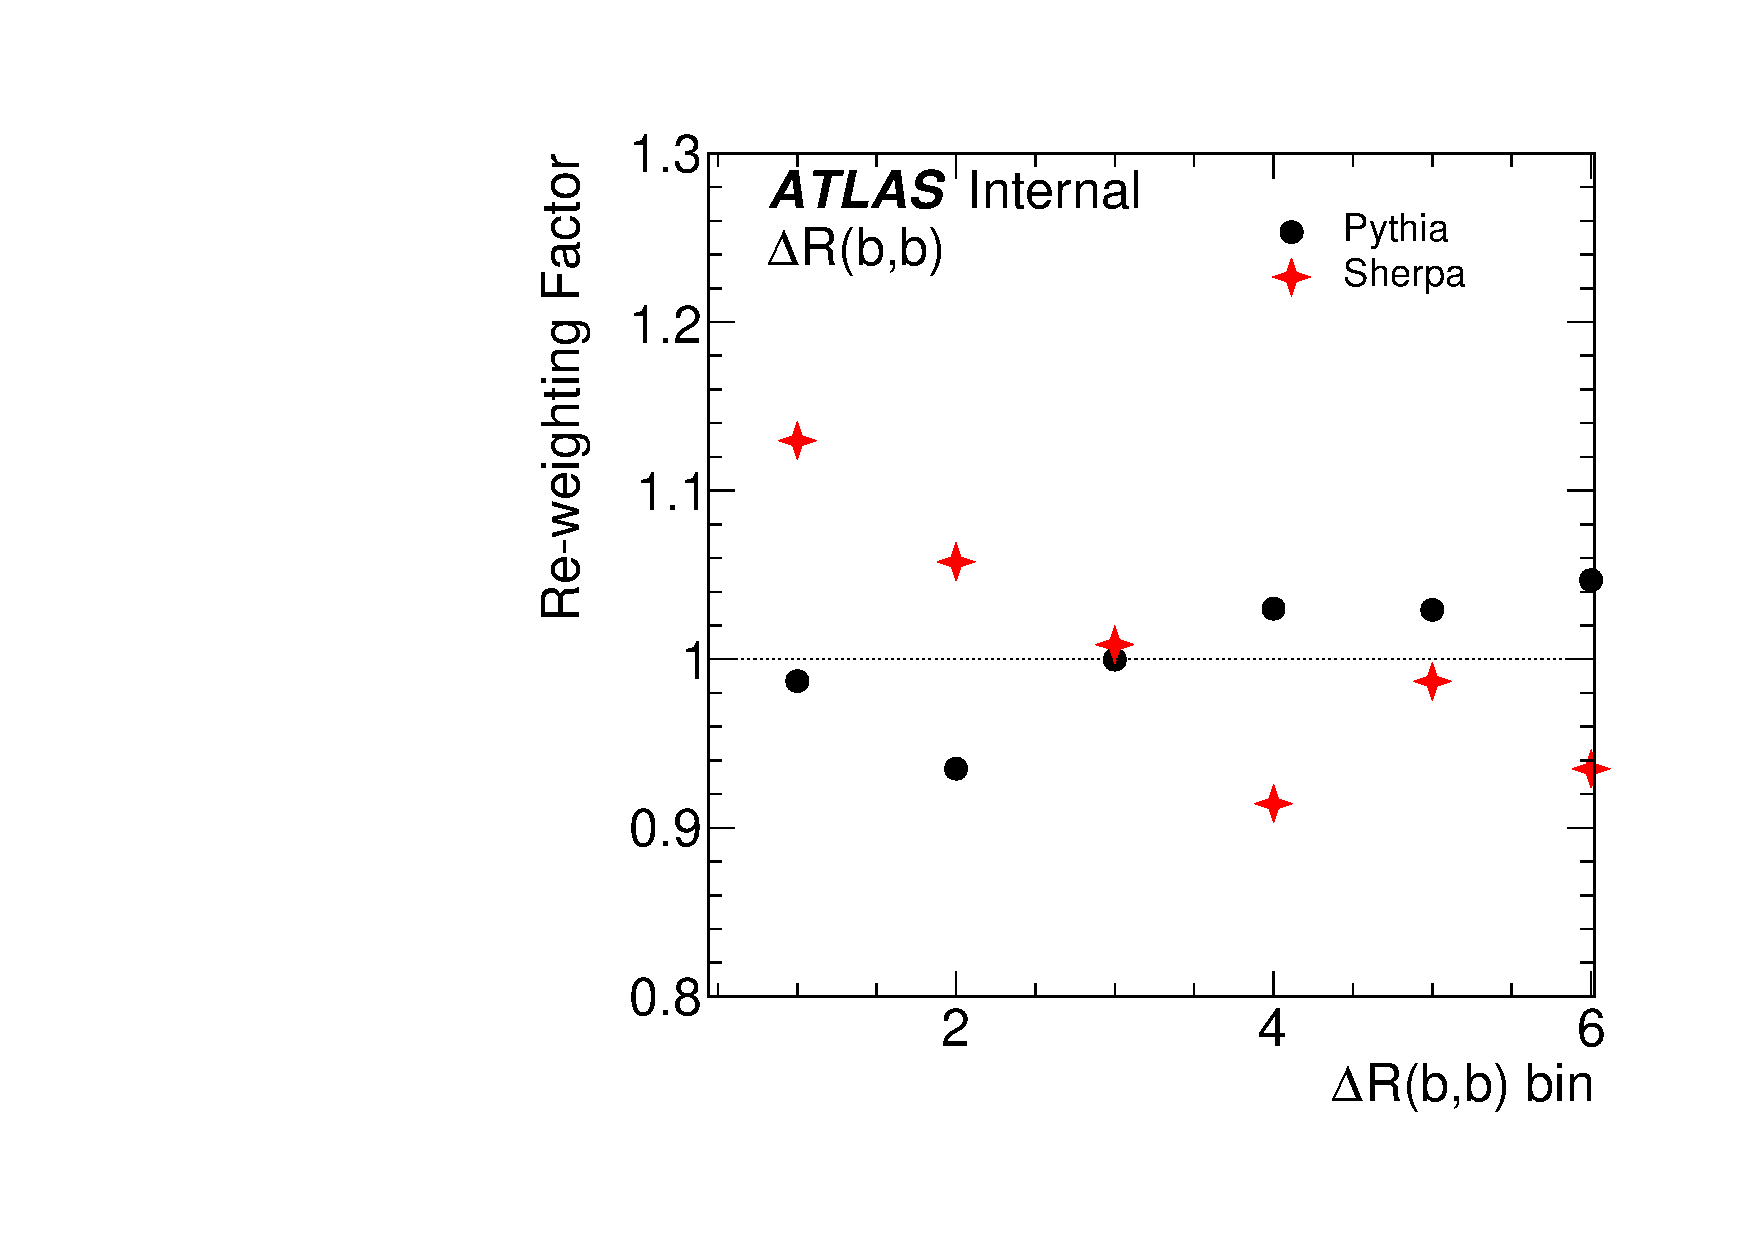
\includegraphics[width=0.45\linewidth]{figures/gbb/Unfolding/noc_factors_dR.pdf}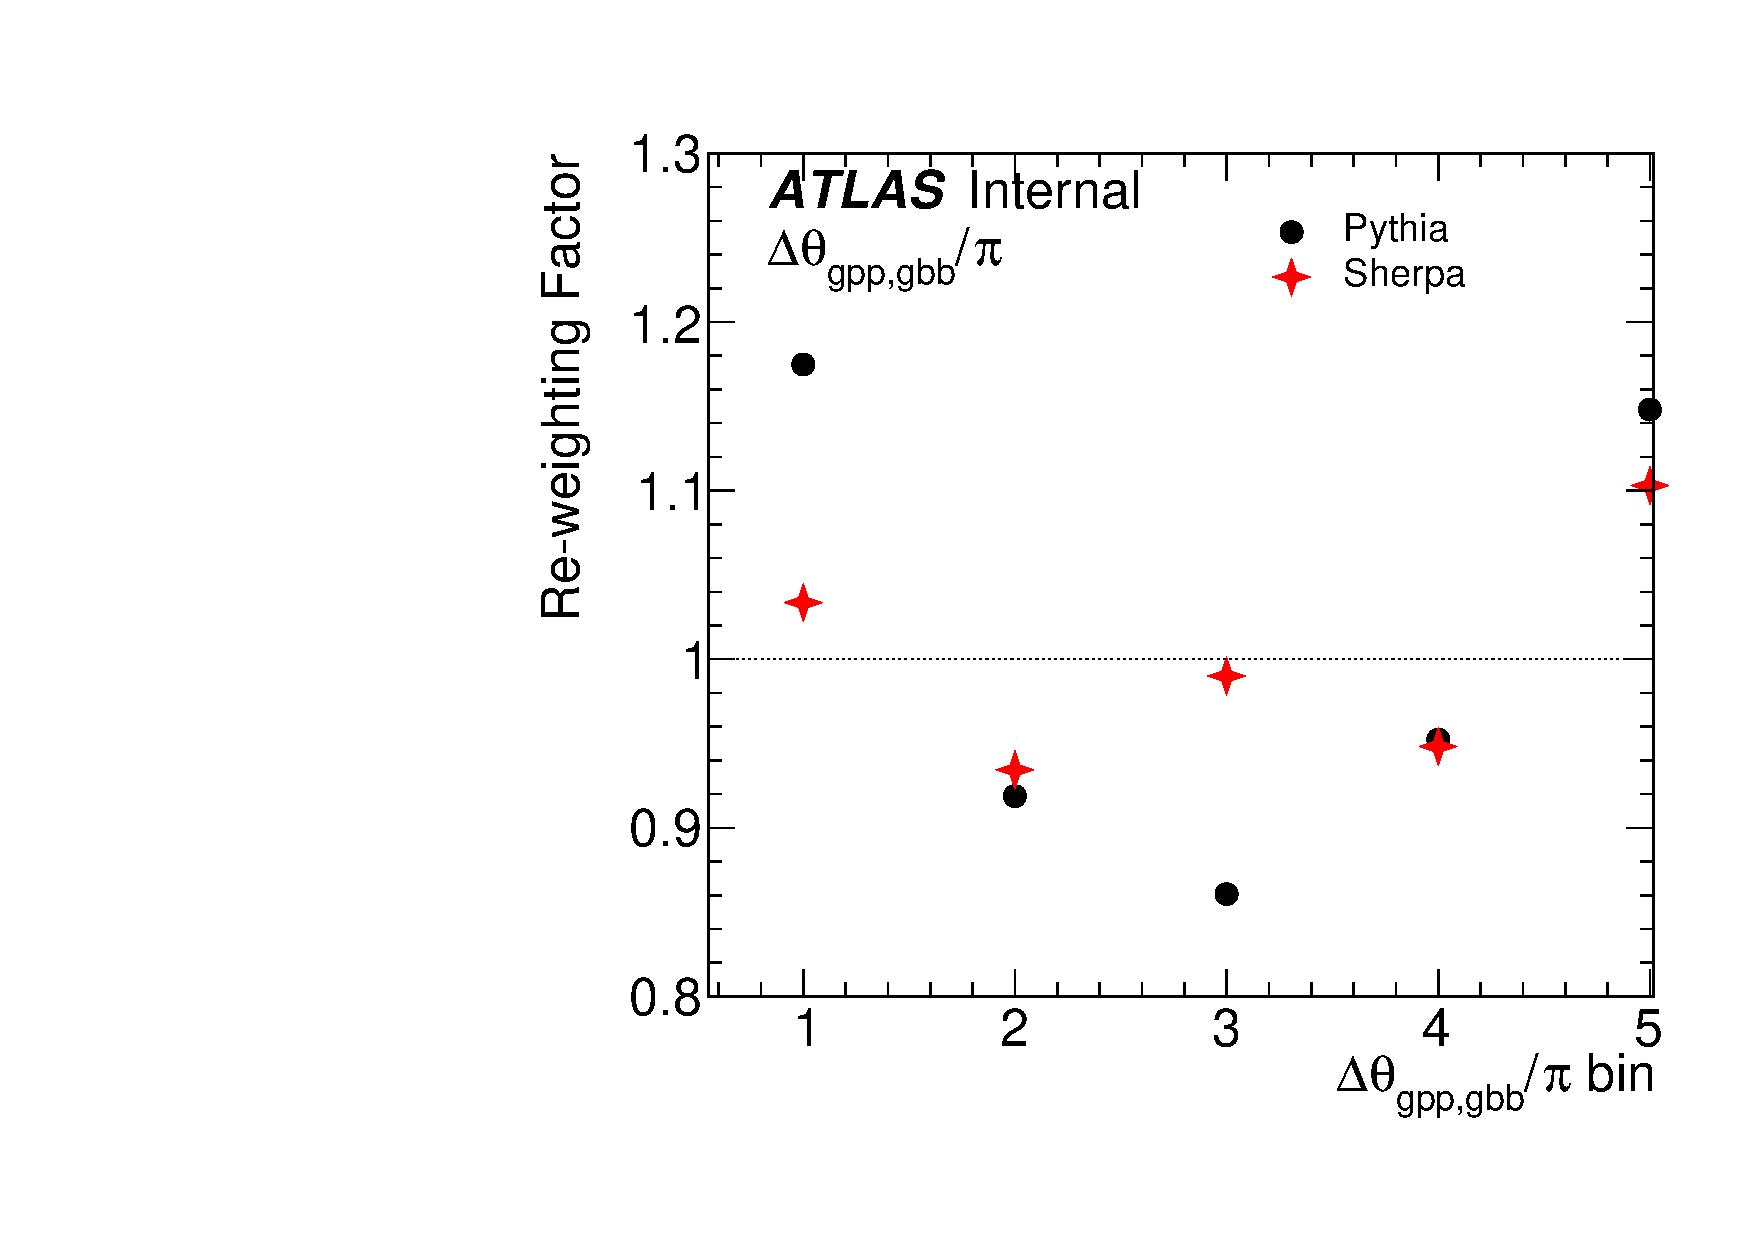
\includegraphics[width=0.45\linewidth]{figures/gbb/Unfolding/noc_factors_dphi.pdf}\\
%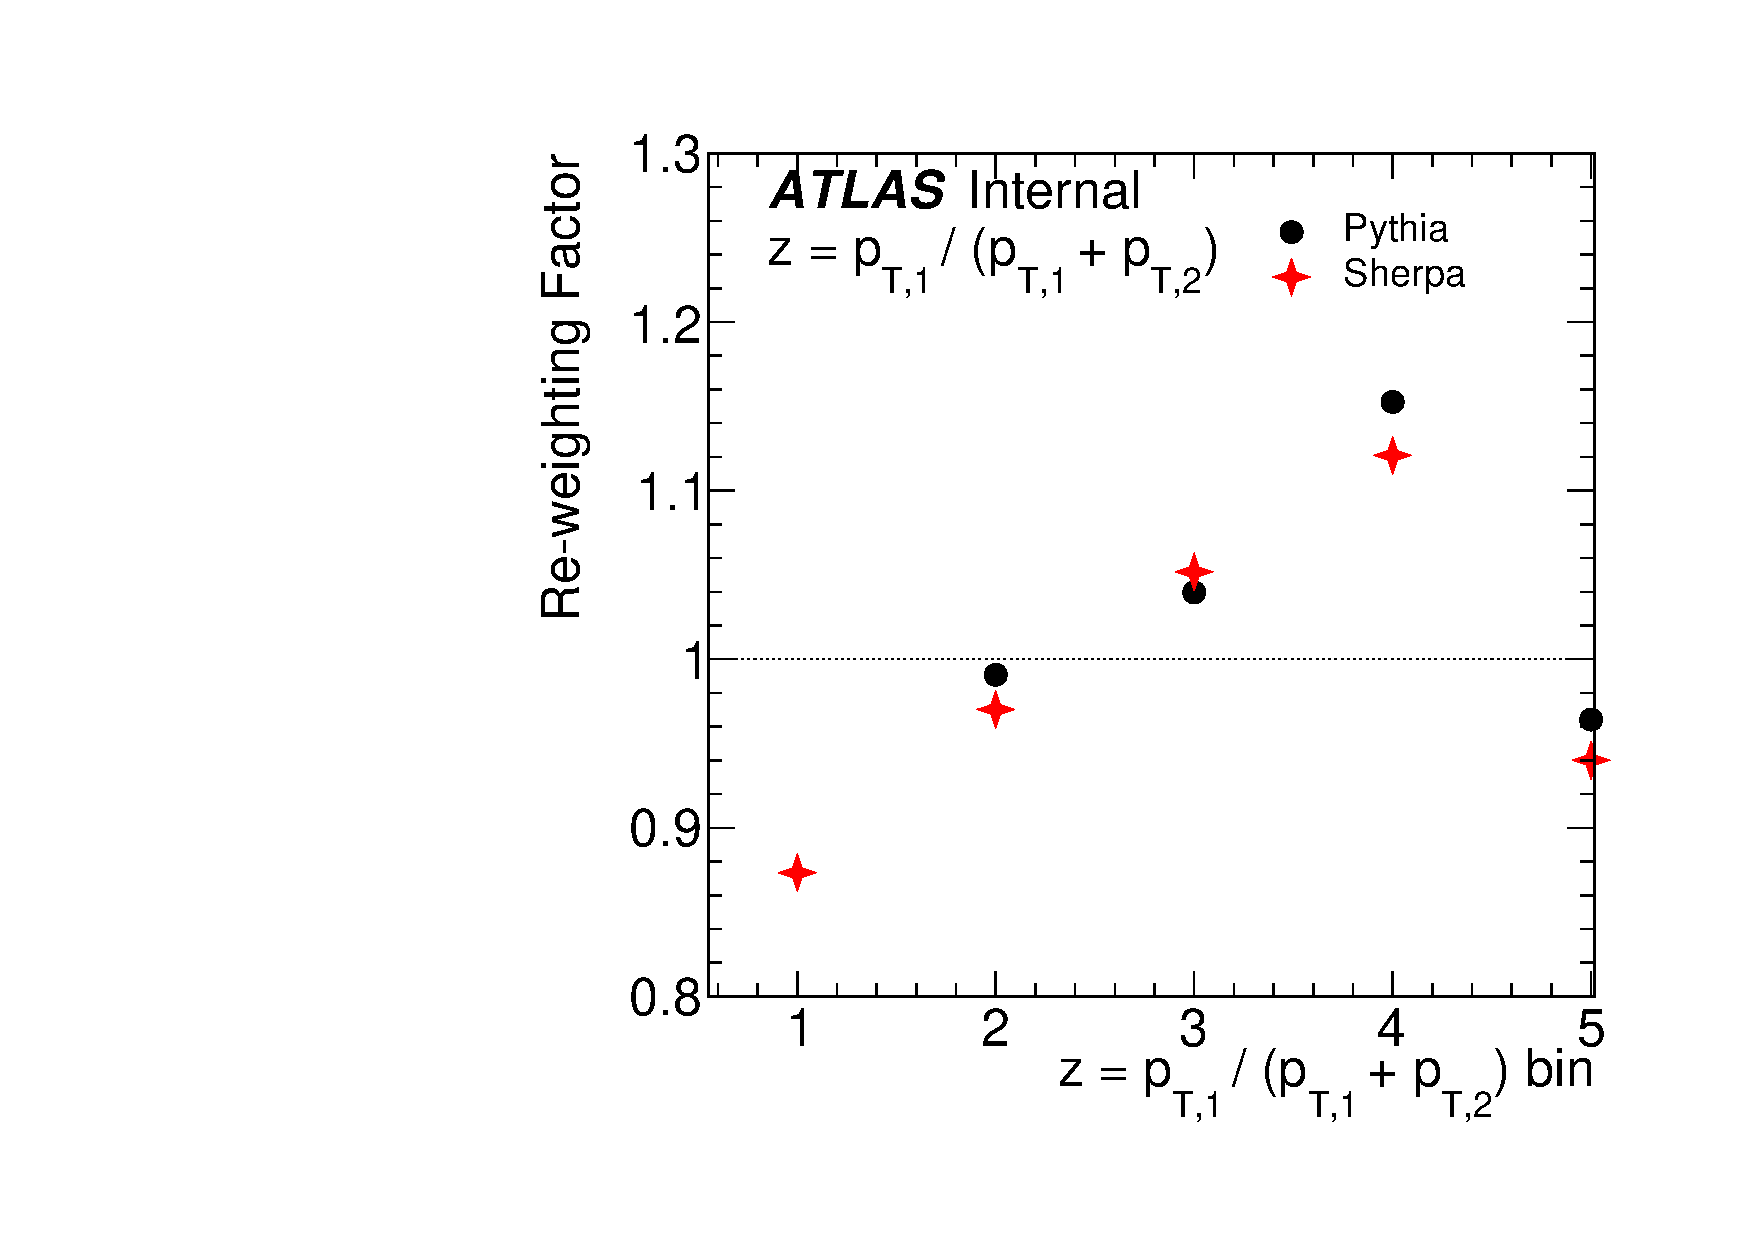
\includegraphics[width=0.45\linewidth]{figures/gbb/Unfolding/noc_factors_ZpT.pdf}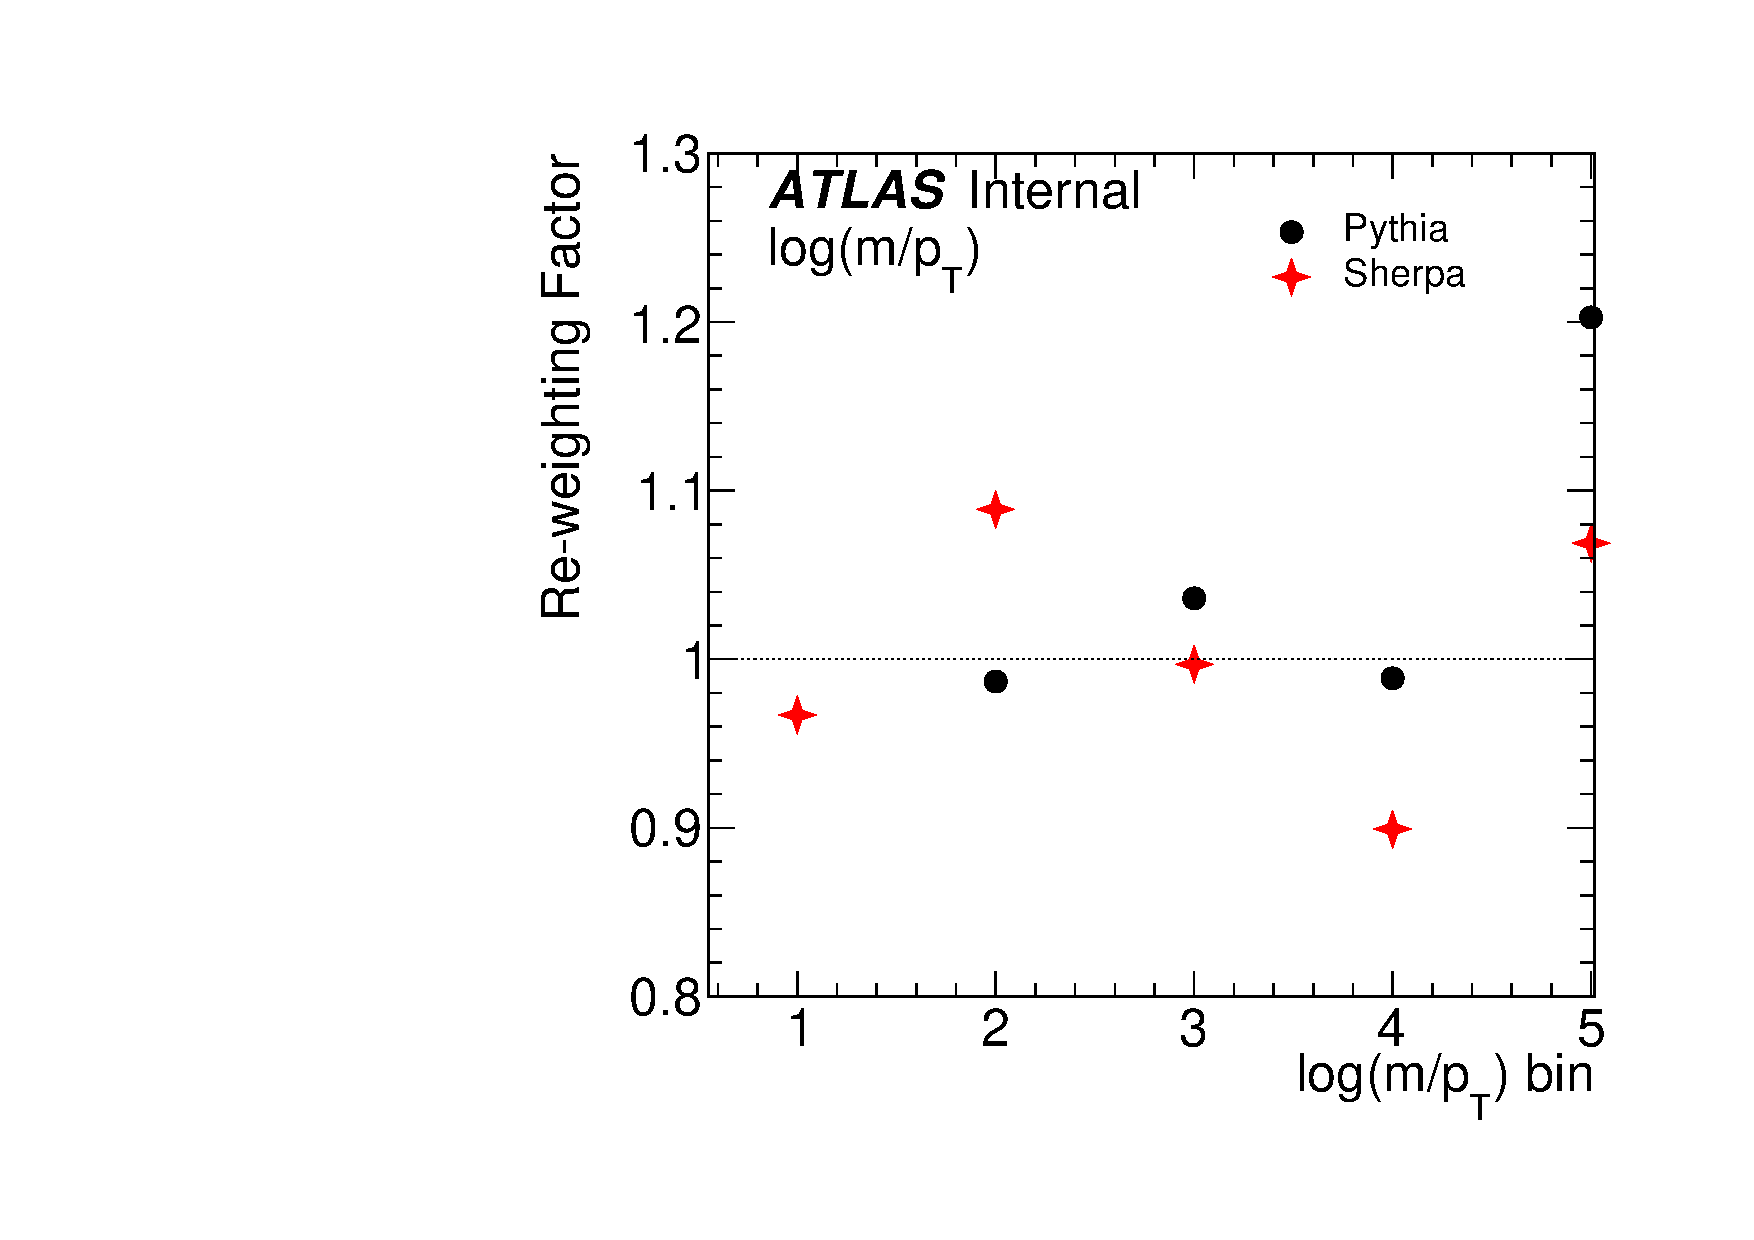
\includegraphics[width=0.45\linewidth]{figures/gbb/Unfolding/noc_factors_fracmasspt.pdf}
%\caption[]{The correction factors applied for the data-driven non-closure uncertainty. } 
%\label{fig:nonclosure1}
%\end{center}
%\end{figure}
%
%\begin{figure}[htpb!]
%\begin{center}
%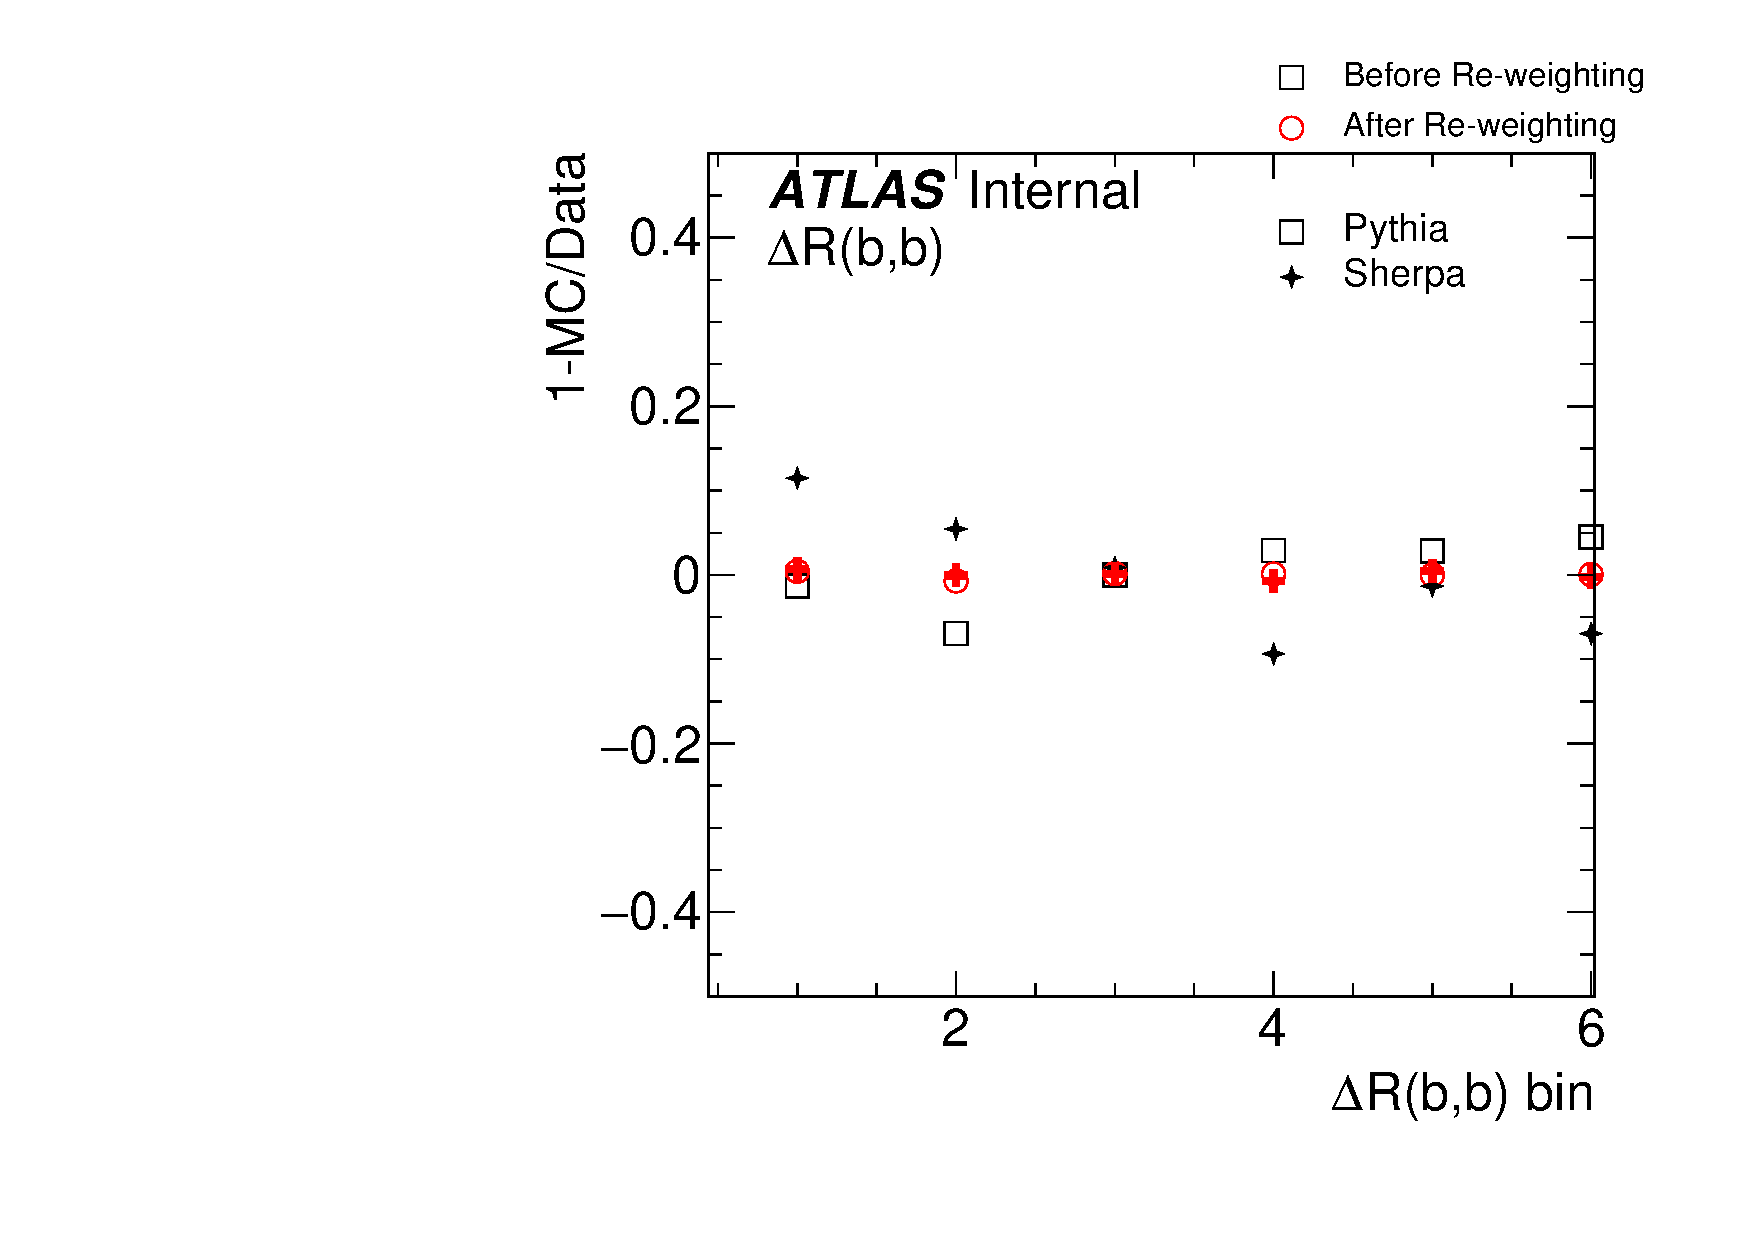
\includegraphics[width=0.45\linewidth]{figures/gbb/Unfolding/noc_datamc_dR.pdf}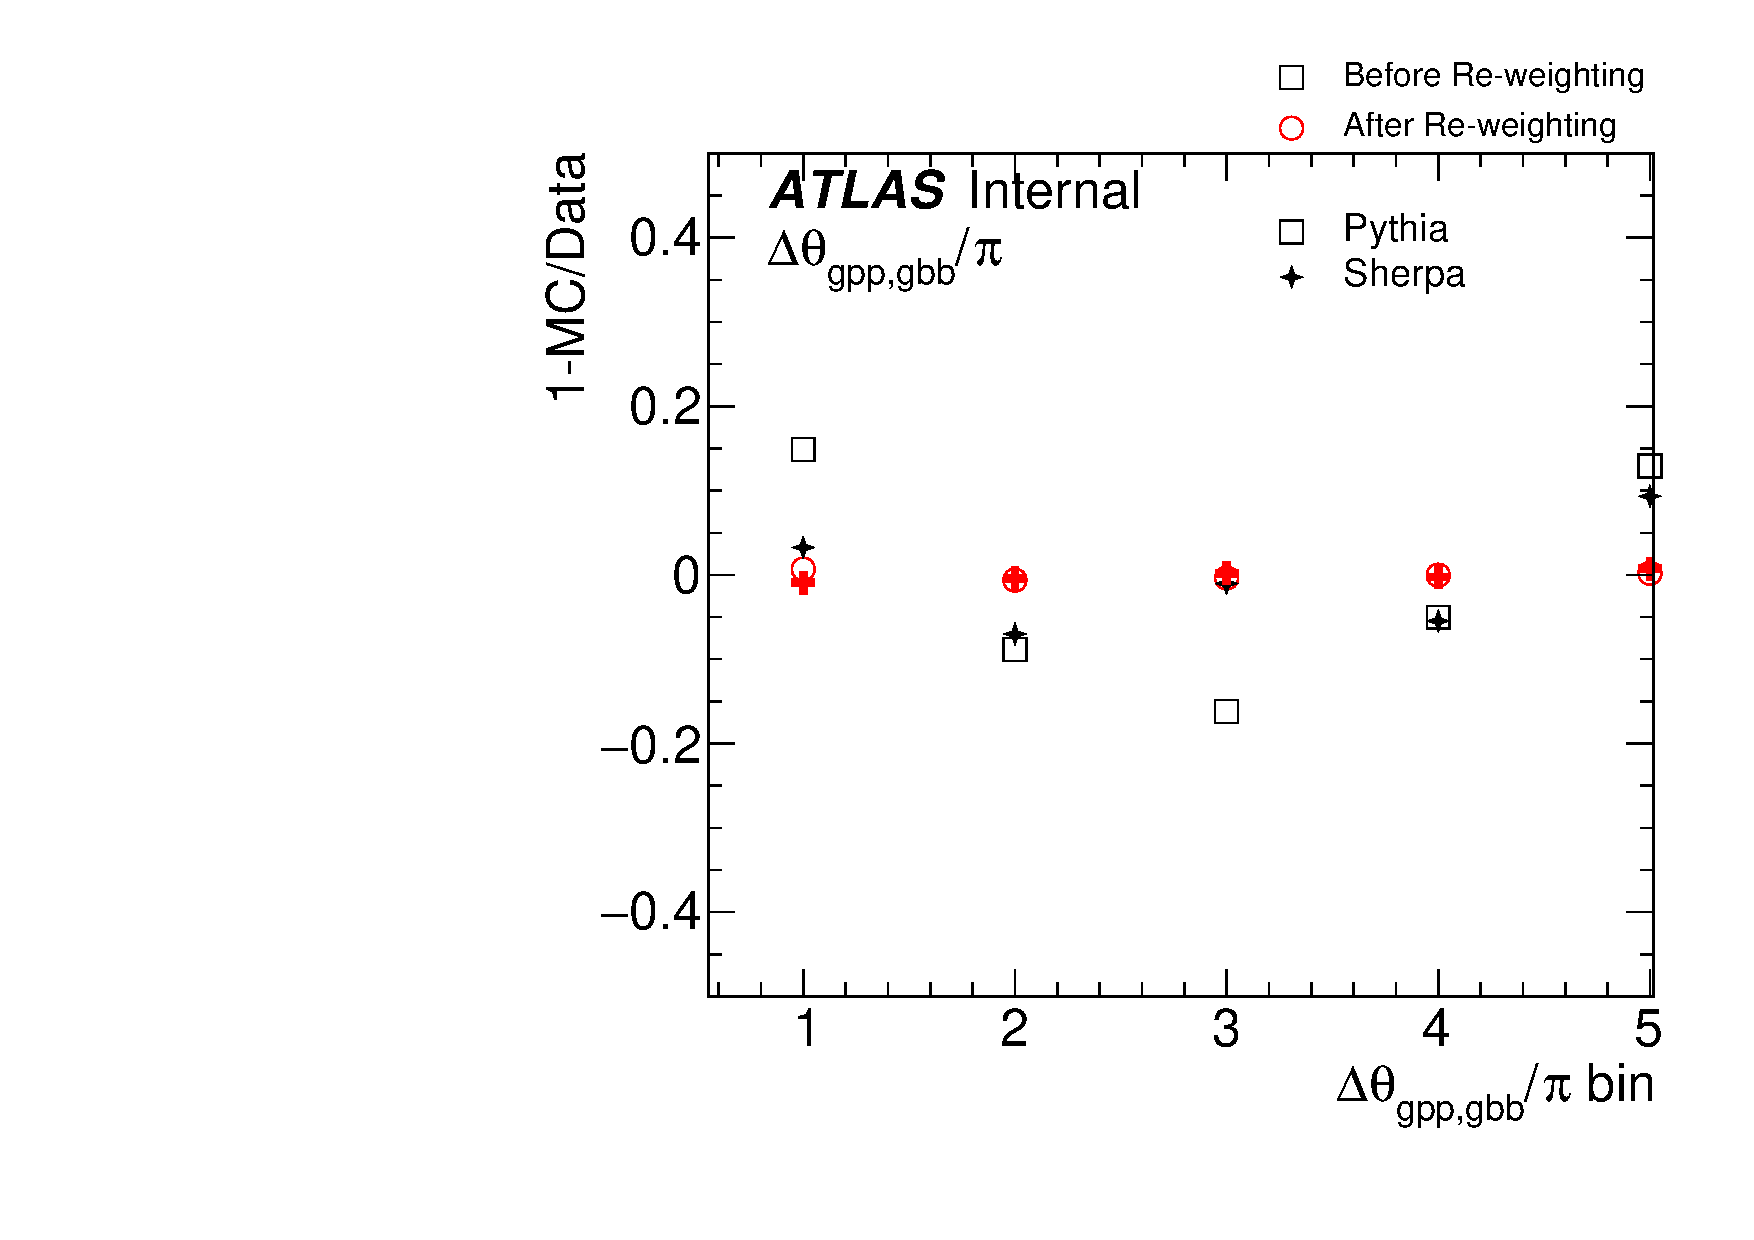
\includegraphics[width=0.45\linewidth]{figures/gbb/Unfolding/noc_datamc_dphi.pdf}\\
%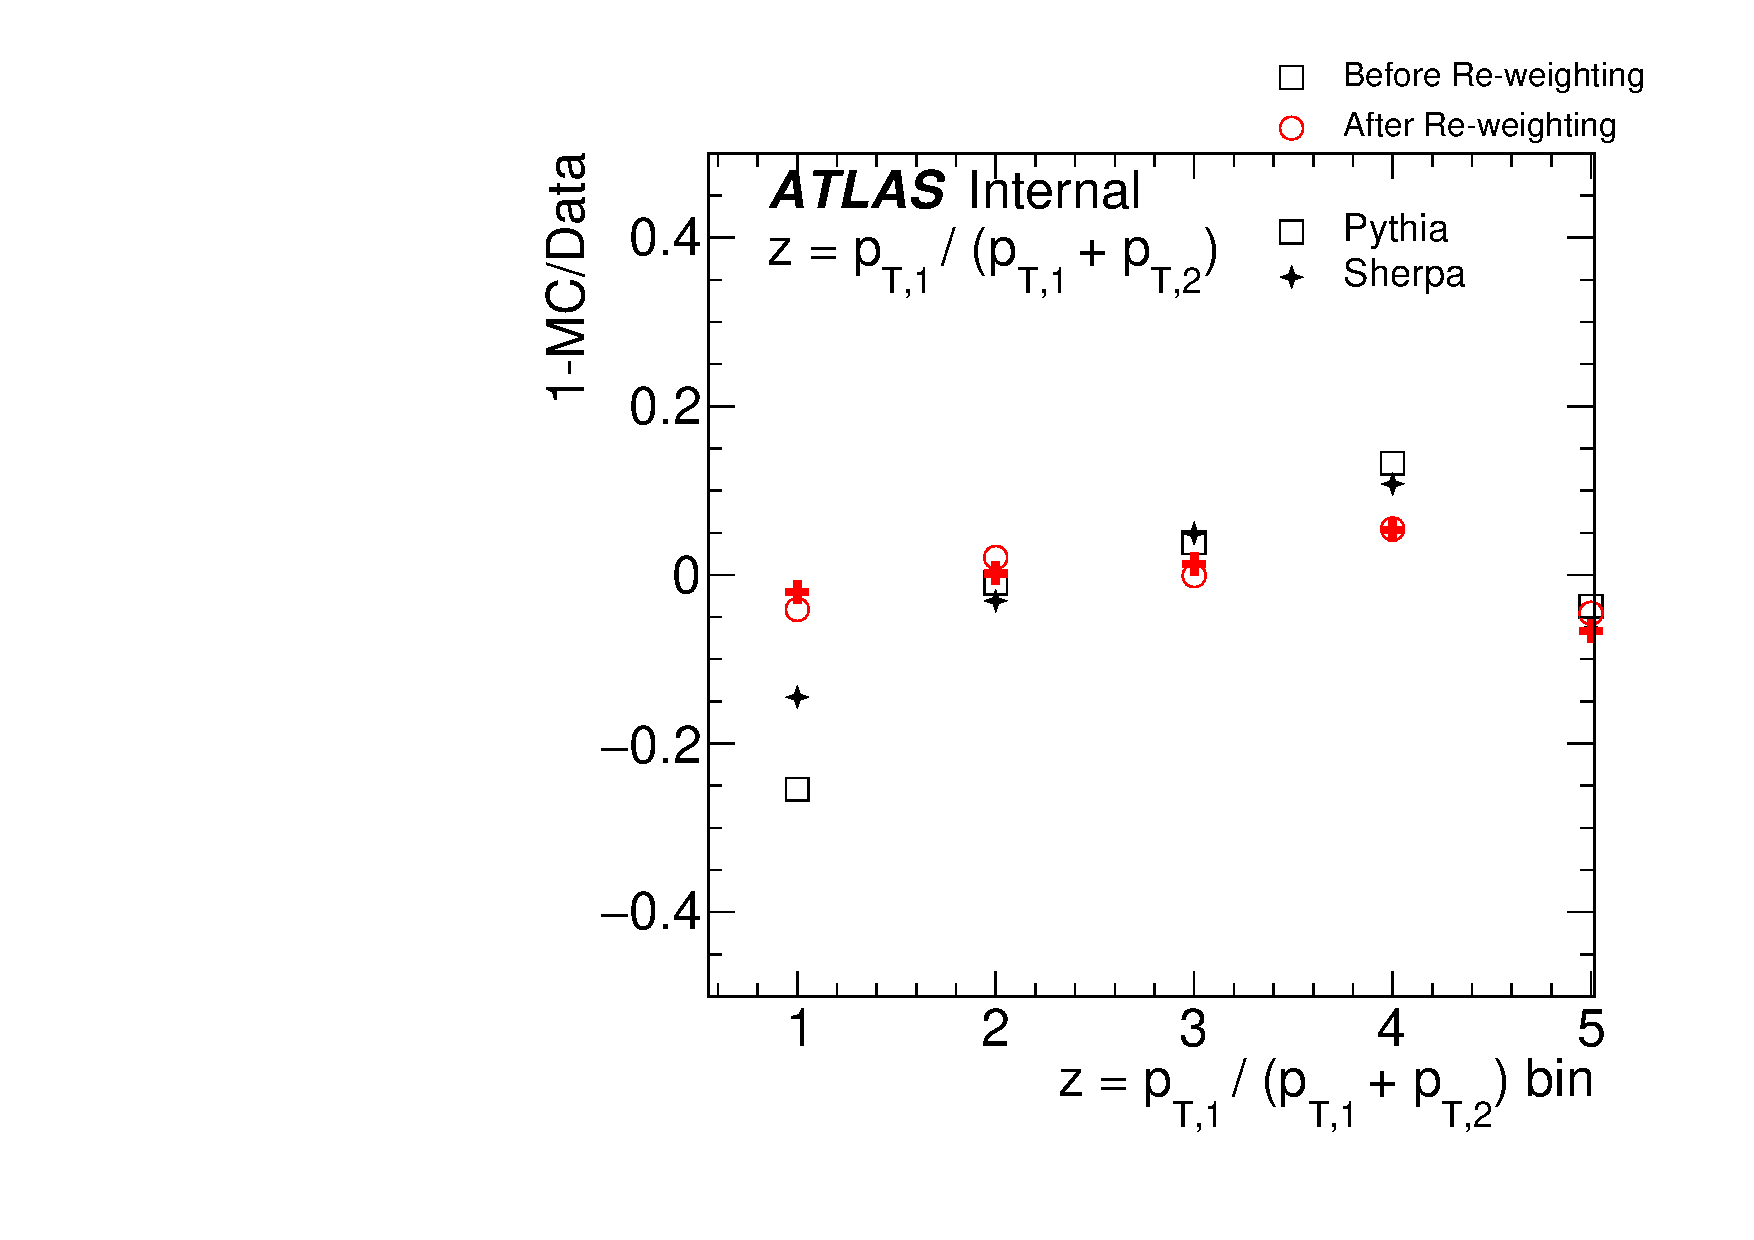
\includegraphics[width=0.45\linewidth]{figures/gbb/Unfolding/noc_datamc_ZpT.pdf}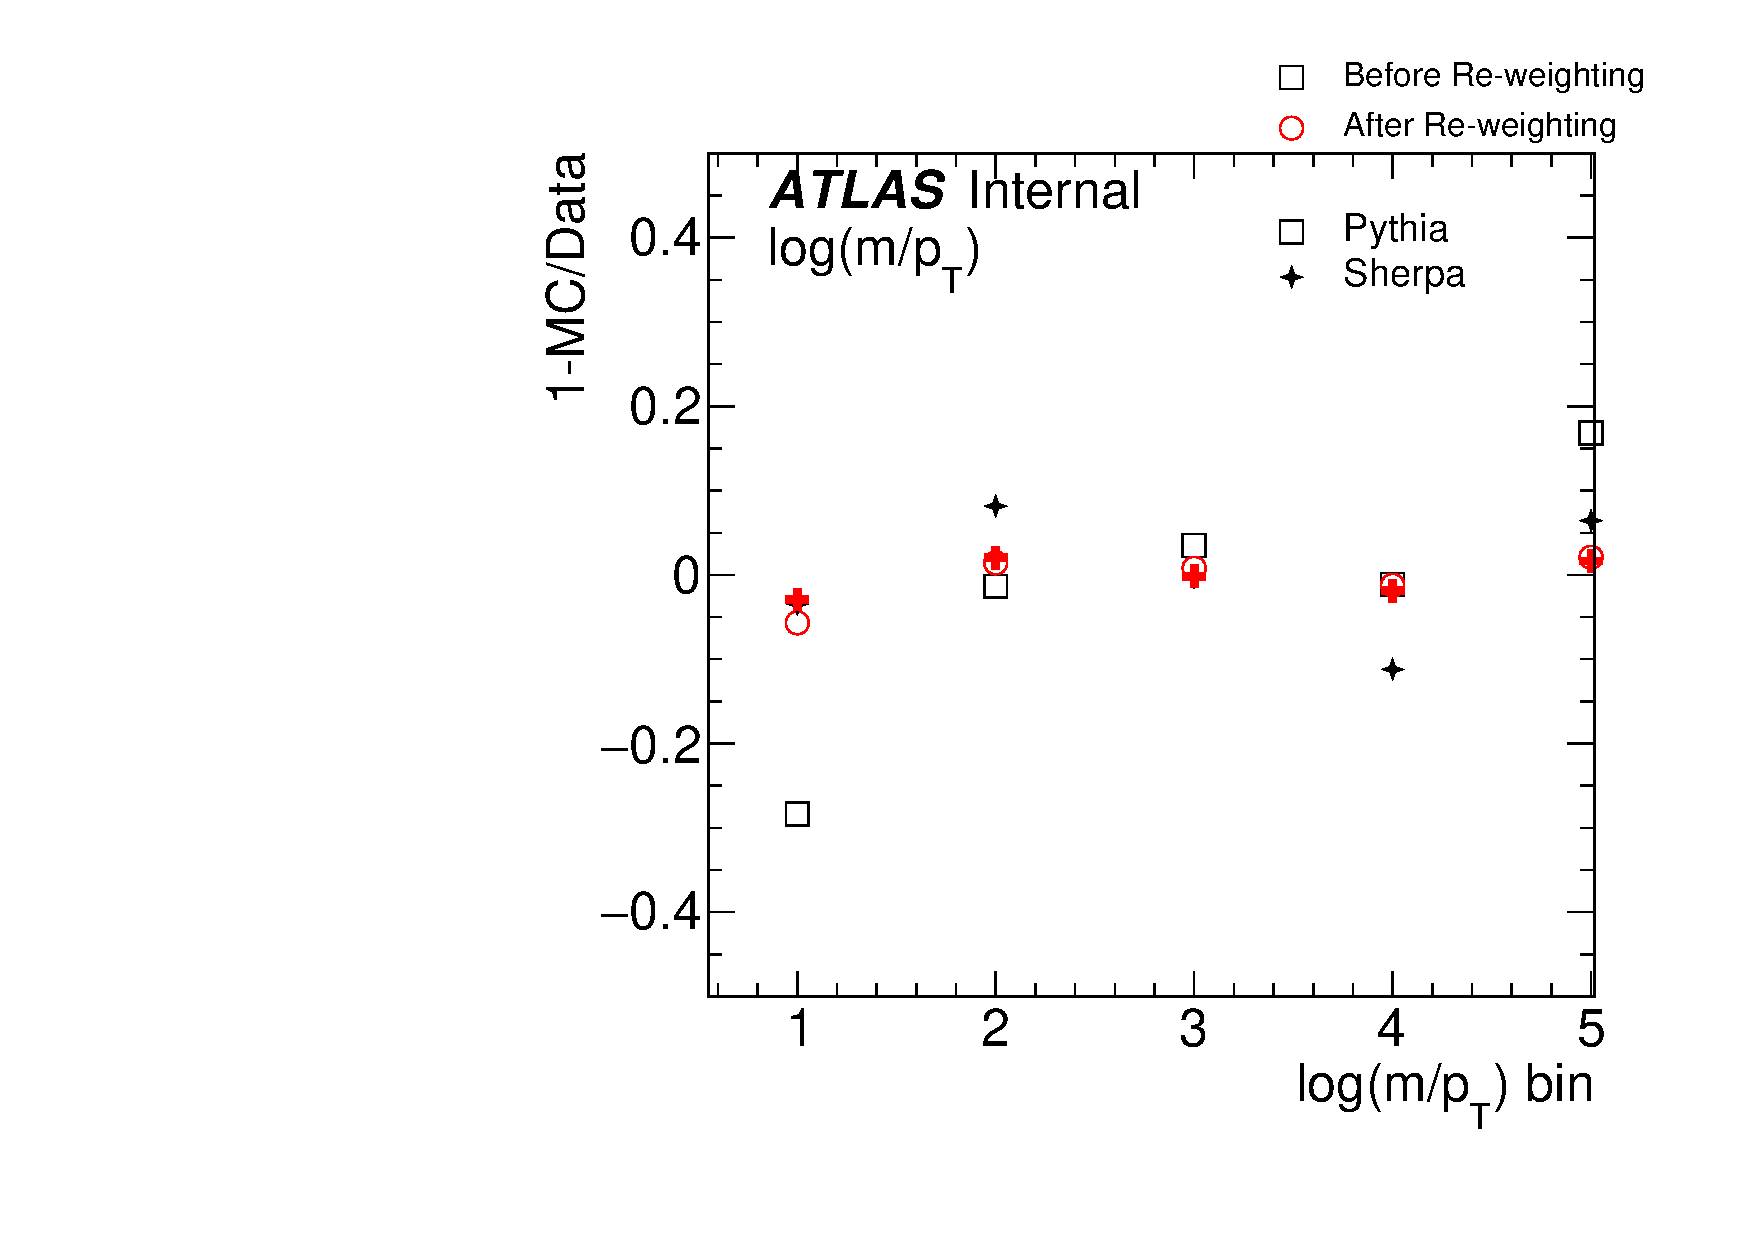
\includegraphics[width=0.45\linewidth]{figures/gbb/Unfolding/noc_datamc_fracmasspt.pdf}
%\caption[]{A comparison of the data/MC difference before and after the re-weighting is applied. } 
%\label{fig:nonclosure2}
%\end{center}
%\end{figure}
%
%\begin{figure}[htpb!]
%\begin{center}
%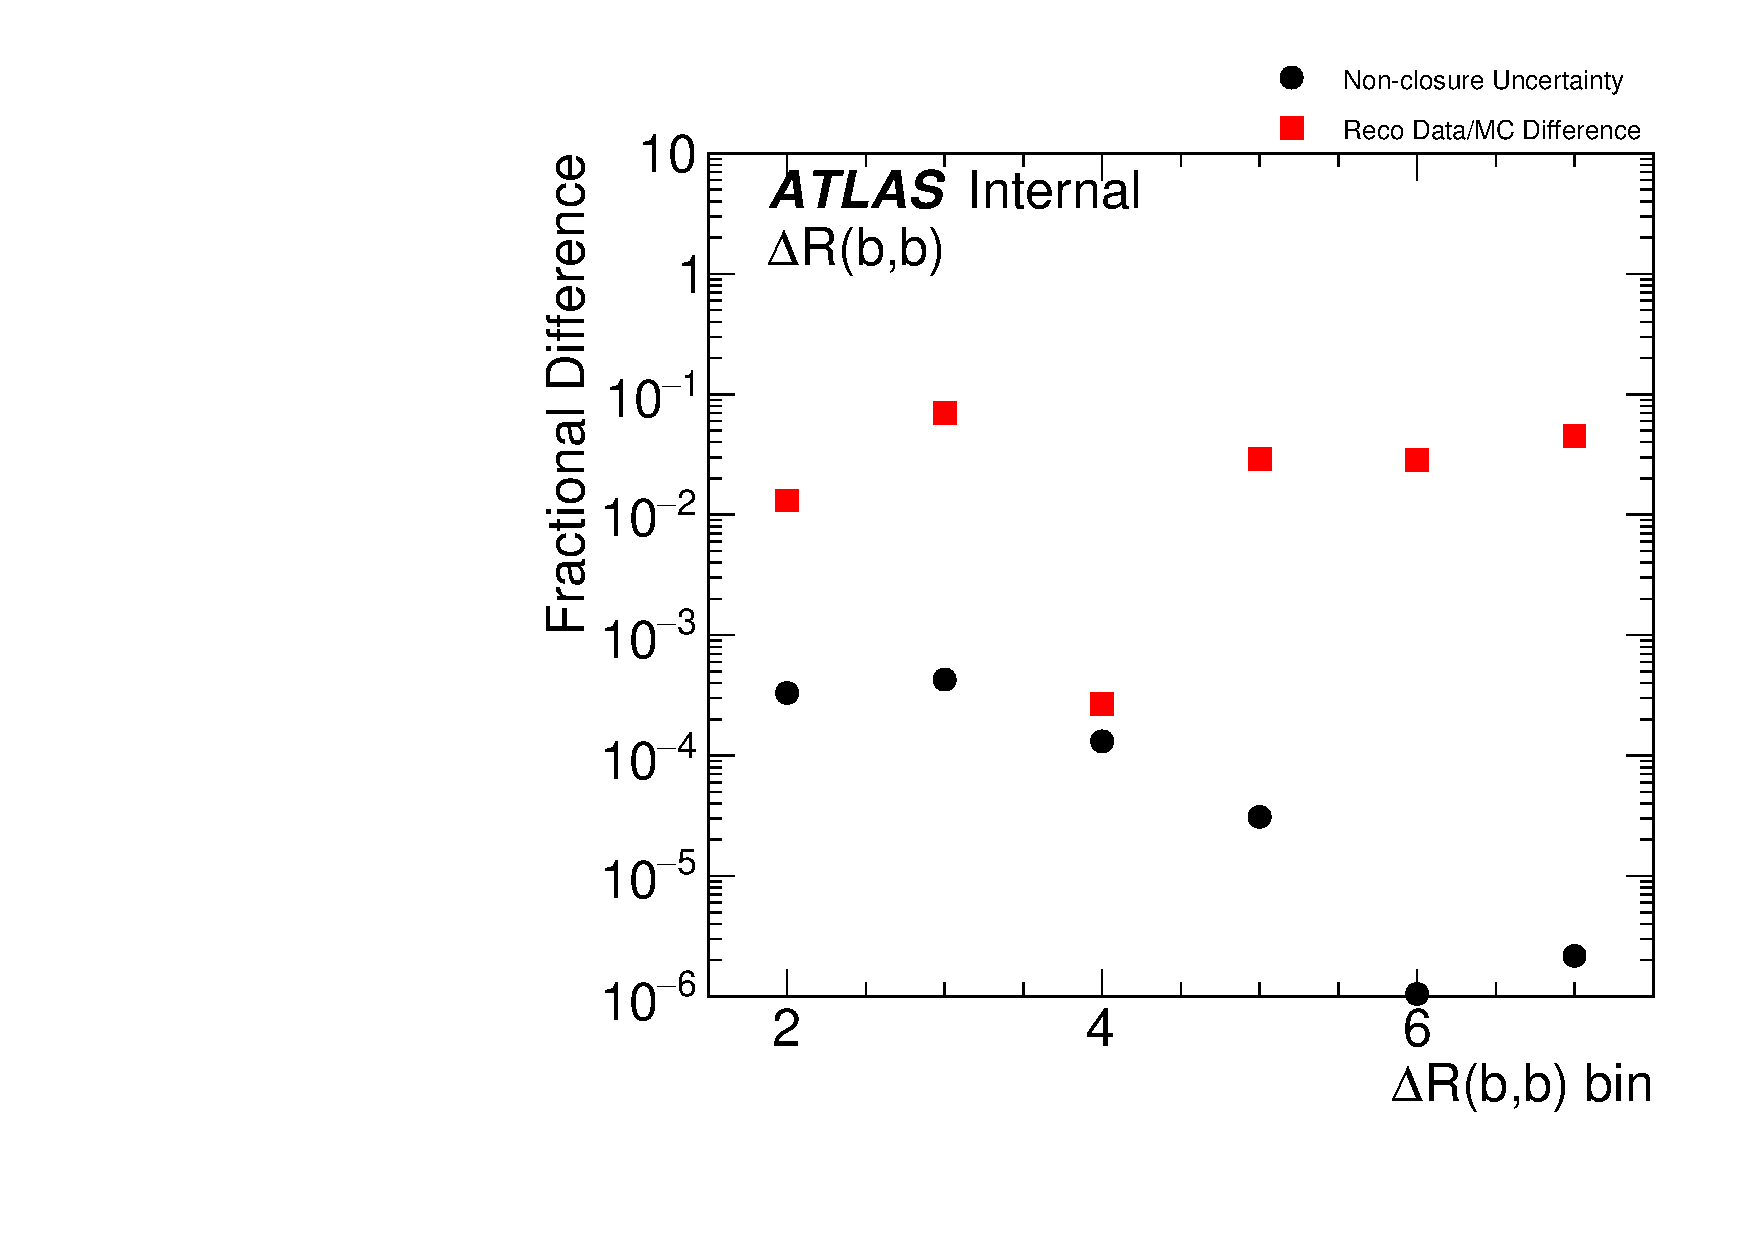
\includegraphics[width=0.45\linewidth]{figures/gbb/Unfolding/non_uncertainty_mean_dR.pdf}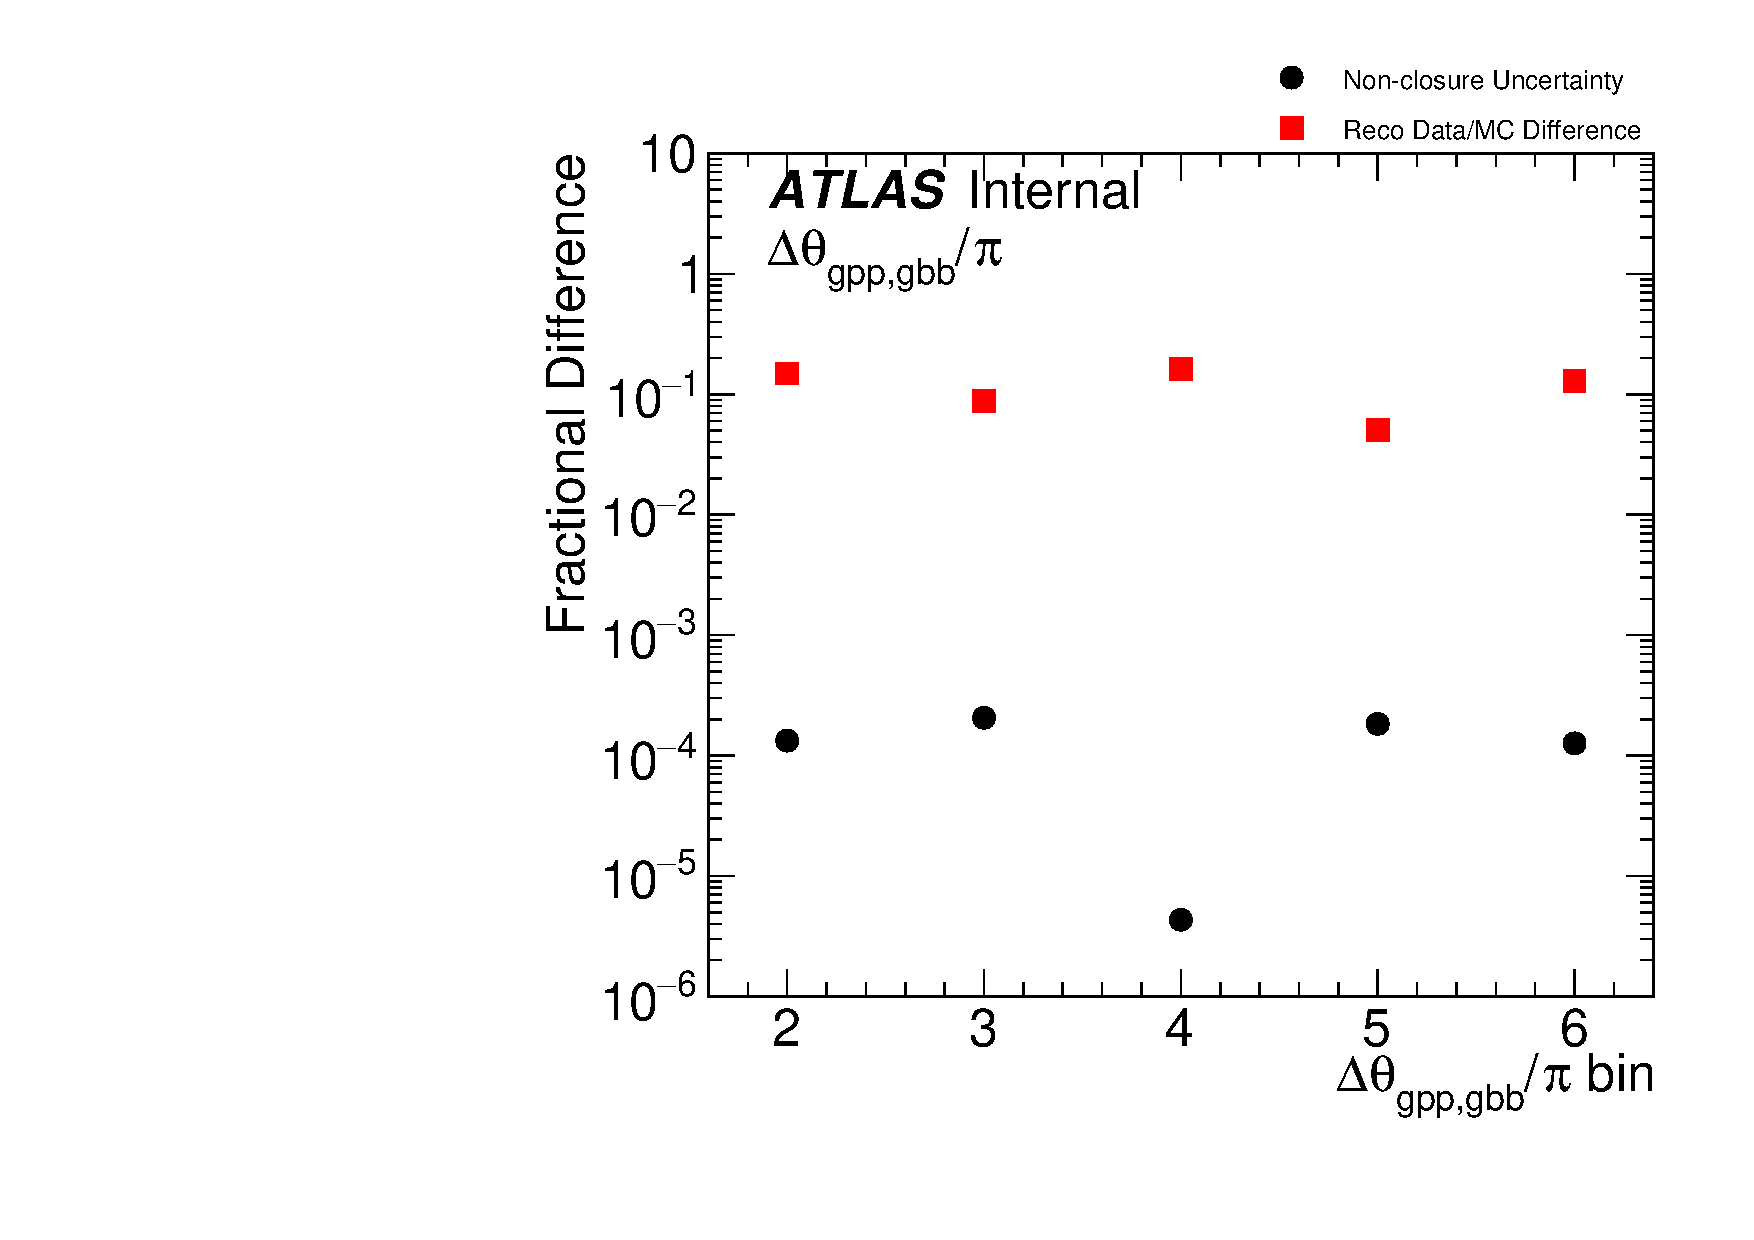
\includegraphics[width=0.45\linewidth]{figures/gbb/Unfolding/non_uncertainty_mean_dphi.pdf}\\
%\includegraphics[width=0.45\linewidth]{figures/gbb/Unfolding/non_uncertainty_mean_ZpT.pdf}\includegraphics[width=0.45\linewidth]{figures/gbb/Unfolding/non_uncertainty_mean_fracmasspt.pdf}
%\caption[]{A comparison of the non-closure uncertainty with the raw data/MC difference. } 
%\label{fig:nonclosure3}
%\end{center}
%\end{figure}



\subsection{Summary}
\label{sec:gbb-systs:overview}

Figure~\ref{fig:syst_overview_deltaR} presents a summary of the unfolded distribution systematic uncertainties. The largest source of uncertainty is theoretical uncertainty. Background subtraction uncertainties and detector uncertainties are the next ones in rank.

\begin{figure}[htpb!]
\begin{center}
\includegraphics[width=0.45\linewidth]{figures/gbb/Unfolding/dR_uncert_summary.pdf}\includegraphics[width=0.45\linewidth]{figures/gbb/Unfolding/dphi_uncert_summary.pdf}\\
\includegraphics[width=0.45\linewidth]{figures/gbb/Unfolding/ZpT_uncert_summary.pdf}\includegraphics[width=0.45\linewidth]{figures/gbb/Unfolding/fracmasspt_uncert_summary.pdf}
\caption[]{A summary of the systematic uncertainties for all four observables. } 
\label{fig:syst_overview_deltaR}
\end{center}
\end{figure}

